\documentclass[
	%parspace, % Add vertical space between paragraphs
	%noindent, % No indentation of first lines in each paragraph
	%nohyp, % No hyphenation of words
	%twoside, % Double sided format
	%draft, % Quicker draft compilation without rendering images
	%final, % Set final to hide todos
]{elteikthesis}[2021/09/20]

% The minted package is also supported for source highlighting
% See minted-intregration.tex for example
%\usepackage[newfloat]{minted}

% Document's metadata
\title{Title of the thesis} % title
\date{2022} % year of defense

% Author's metadata
\author{John Smith}
\degree{Computer Science BSc}

% Superivsor(s)' metadata
\supervisor{John Doe} % internal supervisor's name
\affiliation{Assistant Lecturer} % internal supervisor's affiliation
%\extsupervisor{Jane Doe} % external supervisor's name
%\extaffiliation{Senior Developer} % external supervisor's affiliation

% University's metadata
\university{Eötvös Loránd University} % university's name
\faculty{Faculty of Informatics} % faculty's name
\department{Dept. of Software Technology and Methodology} % department's name
\city{Budapest} % city
\logo{elte_cimer_szines} % logo

% Add bibliography file
\addbibresource{thesis.bib}

% The document
\begin{document}

% Set document language
%\documentlang{hungarian}
\documentlang{english}

% List of todos (not in the final document)
%\listoftodos[\todolabel]

% Title page (mandatory)
\maketitle
\topicdeclaration

% Table of contents (mandatory)
\tableofcontents
\cleardoublepage

% Main content
% ! TeX root = thesis_en.tex

\chapter{Introduction}
\label{ch:intro}

\section{Motivation}

There are programming languages, like Pascal, Ada or BASIC, that distinguish functions that do and do not
have return values,
the latter are known as \emph{procedures}. C family languages do not. Pre-standardisation C language (also known as K\&R C)~\cite{kandr}
did not have \mintinline{CPP}{void} functions,
instead an unspecified return value defaulted to \mintinline{CPP}{int}. This resulted in functions declared with \mintinline{CPP}{int} return value
not returning anything and the supposed return value was unused on purpose. One of its consequences was for example, that for a while if
you wrote a function, that was declared to return \mintinline{CPP}{int} without the return value, the compiler did not act on it. When writing
code in \CC{} we often use functions from C, and a lot of standard library POSIX functions are C functions, taking \mintinline{CPP}{const char *},
\mintinline{CPP}{void *}, returning \mintinline{CPP}{int}.

\section{Problem Statement}
\label{sec:prob-state}

There are quite a few functions whose return value is often ignored, which could lead to potential bugs. Some examples:

\begin{itemize}
    \item POSIX \mintinline{CPP}{read}: returns the number of bytes read; this return value can also indicate errors with it being -1.
    \item POSIX \mintinline{CPP}{scanf}: returns the number of items in the argument list successfully filled; also indicates errors with EOF return.
    \item \mintinline{CPP}{<cstdio>}'s \mintinline{CPP}{std::remove}: return indicates success or error of removal of a file.
    \item \mintinline{CPP}{<algorithm>}'s \texttt{std::remove}: Does not remove. It returns an iterator, and we still need to use container specific erase
    for all elements after this iterator.
    \item \mintinline{CPP}{std::remove_if}: Same as remove.
    \item container-specific \mintinline{CPP}{erase}: Returns an iterator to the next element after the removed.
    \item container-specific \mintinline{CPP}{insert}: Returns an iterator to the first of the new elements inserted.
\end{itemize}

Later, the \mintinline{CPP}{[[nodiscard]]} attribute was introduced~\cite{cppreferencenodiscard} to notify and give warnings to
the user if the return value was unused in case of a function
with this attribute. However, in order to ask the compiler to give warnings on unchecked values, we would need permission to modify the library code.
In case of external source code such as POSIX, STL or any third-party project, we will not have permission to do so.
However, we still need to notify the user on the cases where they do not check non-void return value. This brings us to static analysis.

\section{Static Analysis}

Static analysis is a method to analyse the source code of software projects without performing a real execution of the application.
It is widely used in industry~\cite{statcompare}
to find bugs and code smells during development, to aid in the prevention of bad code that misbehaves in
production~\cite{googlearticle}.
Among various methods, the most important techniques are the ones that are based on pattern matching on a syntactic representation of
the software project.

Clang-Tidy is a declarative, object oriented, strong typed static analysis rule collection that is built upon the LLVM Compiler
Infrastructure's C-family compiler, Clang.
It performs pattern matching on Clang's \emph{``Abstract Syntax Tree''} (AST) representation, and generating diagnostics based on which
analysis modules, called \emph{``checks''}, the user turns on. Pattern matching is an important tool in the industry as well. It can for
example be used for detecting type safety issues~\cite{SZALAY2021111048} or even automatically performing the type migration~\cite{typemig}. An example of an AST can be seen at \cref{fig:ast1}.
We will address both the LLVM library and AST matchers in later chapters of the thesis.

Clang-Tidy's infrastructure is a powerful tool that can even be used to generate \mintinline{CPP}{FixIt}s~\cite{autorefact}, but since a
valid automatic fix does not exist for my checker's warnings, (as it is up to the user to decide whether or not the diagnostics is
valid, or how they should acknowledge the result) this feature will not be used in this thesis.


\begin{figure}[H]
    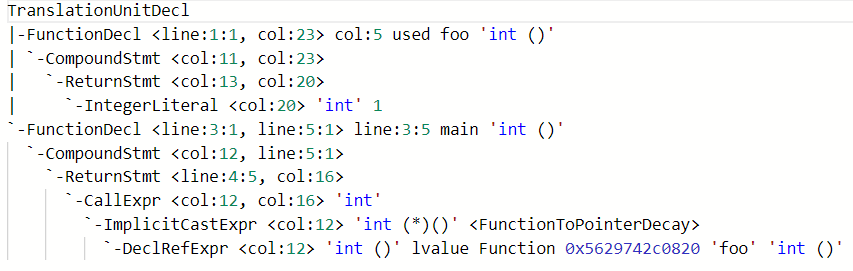
\includegraphics[width=\linewidth]{images/return_foo_ast.png}
    \caption{An example of the Abstract Syntax Tree of \mintinline{CPP}{return foo();}.}
    \label{fig:ast1}
\end{figure}

Let us imagine a checker, that keeps statistics on how many times a return value of a non-\mintinline{CPP}{void} function is used, or otherwise known
as checked. This property is, as we previously stated, important, because there exist a great amount of functions,
whose return value should be checked in most situations but remain unchecked in quite a lot.

\section{Infrastructure Limitations}

Unfortunately, for programming languages in the C family, such as \CC{}, the concept of ``separate translation'' causes issues for static
analysis. As most static analysers are built upon compilers, and in \CC{}, each compiler only sees the local information in the source file
(also known as the \emph{Translation Unit}) it is to compile or analyse (as opposed to project-level knowledge), crucial details
might be hidden, which lowers, or in most cases, completely distorts the accuracy of the analysis.
This means that the way our infrastructure works, a checker like this would be of very limited use.

A function can obviously exist outside of the translation unit of its declaration. If such analysis with our imagined checker is done
separately on each translation unit, it is easy to see how that can affect the outcome. A function might be called 100 times and 
checked 95 times through. We would want to give warnings for the unchecked 5\% of those calls, but if, for example, these are in a 
separate translation unit, then the analysis would return with 0 checks out of 5 calls. We would not want to give warnings to a
function that is unchecked in all 100\% of its calls. The detail of the statistics, that it was only unchecked in 5\% is lost,
unless we use project-level knowledge during our analysis. Consider another example, with code:


% törd el két külön fileba
\begin{listing}
    \begin{minted}{cpp}
// First translation unit

std::vector<int> c{0, 1, 2, 3, 4, 5, 6, 7, 8, 9, 11, 13, 15};

auto iter = c.erase(c.begin());
iter = c.erase(iter + 2, iter + 5);
for (std::vector<int>::iterator it = c.begin(); it != c.end();) {
    if (*it % 2 == 0)
        it = c.erase(it);
    else
        ++it;
}
    \end{minted}

    \begin{minted}{cpp}
// Second translation unit

std::vector<int> c{0, 1, 2, 3, 4};
for (std::vector<int>::iterator it = c.begin();
       it != c.end(); ++it) {
    if (*it % 2 == 0)
        c.erase(it);
}
    \end{minted}

    \caption{An example of the infrastructure's limitations.}\label{lst:motivation-example}
\end{listing}

Here, with separate analysis, the ratio of checked and unchecked calls for \texttt{erase} are 100\% in the first TU (2 checked out of 2 calls),
and 0\% in the second TU (0 checked out of 1call). With project-level knowledge, however we
would get 66\%  (2 checked out of 3 calls). We used erase without a care towards its return value, and this could lead to potential bugs, but without the project
level knowledge, however we can not diagnose it.

The separate analysis could also create false positive results. Imagine we have a function whose return value we could use but it is mostly
optional. We could give our checker a threshold of percentage, to only diagnose unused values if we usually use them in most cases. Again, this
means that with different translation units, we do not know how many times we actually ignored the value and can not use our threshold properly.
This leads to false positive diagnostics.

Unfortunately, the current versions of Clang-Tidy checks can only access what is visible to the compiler, which is a local information.
Several classes of security issues and bad coding patterns might be diagnosed~\cite{googlearticle} if the implemented checks would be 
capable of creating per-compilation knowledge, and reusing the full knowledge about the project during diagnosis.
The work of the thesis is to enhance Clang-Tidy on the infrastructure level to support multi-pass analyses in a generic manner, by 
utilizing the ideas similar to that of MapReduce~\cite{mapreduce}.

This is achieved by allowing individual checks to store check-specific data in a thread-safe location.
A subsequent execution of the analysis will be able to do the pattern matching fine-tuned, with the data stored in the previous step also
available.
To prove the usability of the solution, a new safety and security related check, currently not provided by Clang-Tidy, will be developed
utilizing the new infrastructure created in this work.
In the end, the results of the thesis will allow the international community behind LLVM to develop and make available a wider potential of
checks, as we are planning to upstream the contribution into LLVM. 

\begin{itemize}
    \item \texttt{D124446}~\cite{upstream1}: Add the misc-discarded-return-value check
    \item \texttt{D124447}~\cite{upstream2}: Add infrastructure support for running on project-level information
    \item \texttt{D124448}~\cite{upstream3}: Add project-level analysis support to misc-discarded-return-value
\end{itemize}

\section{Related Works}

The topic of cross translation unit analysis shares other different solutions and implementations as well, one great example is
Clang CTU~\cite{clangCTU}.
As previously stated, the infrastructure enhancement follows the philosophy of MapReduce~\cite{mapreduce}.
There exists a static analysis rule in Coverity Scan static analysis tool, that is similar to our checker~\cite{coverity}.


\section{Thesis layout}

After the Introduction, in \Cref{ch:user}, the User Guide will have instructions on how to download, compile and set up the
static analysis tool, and how to run it on a \CC{} project. In \Cref{ch:impl}, the Developer Guide will explain how the
checker, and the infrastructure itself works, in detail.

\cleardoublepage

\chapter{User documentation}
\label{ch:user}

Both the changes in the Clang-Tidy infrastructure and our new checker obviously focuses heavily on LLVM's Clang-Tidy.
Clang-Tidy is a clang-based C++ “linter” tool. Its purpose is to provide an extensible framework for diagnosing and fixing
typical programming errors, like style violations, interface misuse, or bugs that can be deduced via static analysis.
Clang-Tidy is modular and provides a convenient interface for writing new checks. % https://clang.llvm.org/extra/clang-tidy/
\par This tool can be found in the LLVM project repository. % https://github.com/llvm/llvm-project

\section{Install guide}

\subsection{System Requirements}

Table 2.1 shows the system requirements and supported compilers for building
LLVM. The checkers were developed with Ubuntu 20.04 and tested on Ubuntu 18.04, and WSL Ubuntu 20.04.
\par Building and using LLVM's Clang-Tidy takes a lot of time on weaker computers. The minimum recommended memory size
for building is 16 GB, the optimal amount is 64 GB of memory. % continue with the recommendation  

\begin{table}[H]
	\centering
	\begin{tabular}{ | m{0.33\textwidth} | m{0.33\textwidth} | m{0.33\textwidth} | }
		\hline
		\textbf{Operating System} & \textbf{Processor Architecture} & \textbf{Compiler} \\
		\hline \hline
		Linux & x861 & gcc, clang \\
		\hline
		Linux & amd64 & gcc, clang \\
		\hline
		Linux & arm & gcc, clang \\
		\hline
		Linux & Mips & gcc, clang \\
		\hline
		Linux & PowerPC & gcc, clang \\
		\hline
		Solaris & V9 & gcc \\
		\hline
		FreeBSD & x861 & gcc, clang \\
		\hline
		FreeBSD & amd64 & gcc, clang \\
		\hline
		NetBSD & x861 & gcc, clang \\
		\hline
		NetBSD & amd64 & gcc, clang \\
		\hline
		macOS2 & PowerPC & gcc \\
		\hline
		macOS & x86 & gcc, clang \\
		\hline
		Cygwin & x86 & gcc \\
		\hline
		Windows & x86 & Visual Studio \\
		\hline
		Windows64 & x86-64 & Visual Studio \\
		\hline
	\end{tabular}
	\caption{System requirements and supported compilers for building LLVM}
	\label{tab:example-1}
\end{table}

Software requirements include (at least) GCC version 7.1.0, CMake version 3.13.4, Python version 3.6 and GNU Make version 3.79. % https://llvm.org/docs/GettingStarted.html#requirements

\subsection{Building from source}

These commands will compile LLVM from source. The building process with parameters can be found on the README.md of
LLVM project Github repository, or the Getting Started page of Clang documentation. These are the commands I used for
the compilation. 
% https://github.com/llvm/llvm-project#readme and https://clang.llvm.org/get_started.html

\begin{lstlisting}[language={bash}]
	# On windows, git clone --config core.autocrlf=false https://github.com/llvm/llvm-project.git
	git clone https://github.com/llvm/llvm-project.git
	cd llvm-project
	mkdir Build

	# cmake -S llvm -B build -G <generator> [options]
	cd Build/
	cmake \
		-DCMAKE_EXPORT_COMPILE_COMMANDS=ON \
		-DLLVM_ENABLE_PROJECTS="llvm;clang;clang-tools-extra" \
		-DLLVM_TARGETS_TO_BUILD="X86" \
		-DLLVM_APPEND_VC_REV=OFF \
		-DLLVM_ENABLE_BINDINGS=OFF \
		-DLLVM_USE_RELATIVE_PATHS_IN_FILES=OFF \
		-DBUILD_SHARED_LIBS=ON \
		-DLLVM_USE_LINKER="lld" \
		-DLLVM_PARALLEL_LINK_JOBS=3 \
		-DCMAKE_BUILD_TYPE=Release \
		-DLLVM_ENABLE_DUMP=ON \
		-DLLVM_ENABLE_ASSERTIONS=ON \
		-G Ninja \
		../llvm
	
	# cmake --build build [-- [options] <target>] or your build system specified above directly.
	ninja -j12 clang-tidy llvm-symbolizer
\end{lstlisting}

Explanation for some flags: at \texttt{DLLVM\_USE\_LINKER} we can change the linker we are using, either Gold or LLD (Linker for LLVM). The
latter needs to be installed. \texttt{DLLVM\_PARALLEL\_LINK\_JOBS} and -j at Ninja sets the CPU capacity. The recommended amount for
\texttt{LINK\_JOBS} is one quarter of the amount of cores, and Ninja job amount should be cores - 2. I used these commands on a
server with 32 GB memory and 14 CPU cores.


\section{Running by Translation Units}

You can give Clang-Tidy multiple translation units to run on, and it will give you diagnosis separately for each one. You run it by
using \lstinline{clang-tidy -checks='-*,misc-discarded-return-value' -p ./Build a/main.cpp b/main.cpp},
where the "checks" first disables all checkers with -*, then enables our checker, the flag "p" gets the build path and finally
we give the paths to our code. Here we are getting two separate diagnoses for our two separate files or translation units.

% output example from one of the code compass SINGLE runs

\section{Multiple Phase Version}

The updated infrastructure contains two new flags for running Clang-Tidy, multipass-phase and multipass-dir.
Multipass-phase is an enum flag, that has three values, "collect", "compact" and "diagnose" with the latter as default.
Multipass-dir needs a path to a directory where the checkers that support the collect feature can dump their collection datas
that they are going to compact and use later.

\subsection{Collect}

Collect phase, as the name suggest, will have the checkers collect data on each translation unit and write them into unique yaml
files to later reuse this data. This is how you normally run collect phase on the desired files:

\begin{lstlisting}[language={bash}]
	clang-tidy \
	-checks='-*,misc-discarded-return-value' \
	--multipass-phase=collect \
	--multipass-dir='MyCollectionDirectory' \
	-p ./Build \
	a/main.cpp b/main.cpp
\end{lstlisting}

What Discarded Return Value checker (or DRV) does in this phase, is count the amount the declared non-void functions were called,
and count the amount that these function's return values were checked. After finishing counting in one translation unit, it writes the
collected numbers and function names into a yaml file as a struct.  
\par After collecting, you do not get any diagnosis or output text, but the desired amount of (in this case 2) yaml files are going to
be generated.

% létrejött file mutatása

\subsection{Compact}

Compact phase will iterate through the collected data per checker and have the checkers read, use and compact all the data collected
into one yaml file.

\begin{lstlisting}[language={bash}]
	clang-tidy \
	-checks='-*,misc-discarded-return-value' \
	--multipass-phase=compact \
	--multipass-dir='MyCollectionDirectory' \
	-p ./Build \
	a/main.cpp b/main.cpp
\end{lstlisting}

DRV reads the data on each function back and constructs new data similar to the previous ones. If one function is called in multiple
translation units, then it simply adds the numbers from the TU's yaml file to the new structure. After it is finished, the data is
written into a single yaml file.
\par This phase does not write anything on standard output either, but will construct the compacted yamls per checker.

% létrejött file mutatása

\subsection{Diagnose}

For backwards compatibility, the default diagnose phase, if compact has not happened for a checker, will do exactly what the non-multiple
phase Clang-Tidy did, give diagnosis 

\begin{itemize}
	\item Collect phase, as the name suggest, will have the checkers collect data on each translation unit and write them into yaml files.
	\item Compact phase will have the checkers read, use and compact all the data collected into one yaml file.
	\item Diagnose phase has two types of behaviour:
	\begin{itemize}
		\item If compact had been run for the checker, it will read and use the compacted data and diagnose accordingly.
		\item Otherwise the checker will act as it would have originally, before the feature and the infrastructure was introduced.
	\end{itemize}
\end{itemize}

Here is an example of a project with two files (of the same name) in different folders, and how I run this from terminal.
The original procedure of diagnosis would have been to simply write


Instead of this, we will have do it in different phases:

\begin{lstlisting}[language={bash}]
	# Pre-collection diagnosis (The phase and directory flags are unneeded in this scenario)
	clang-tidy \
	-checks='-*,misc-discarded-return-value' \
	--multipass-phase=diagnose \
	--multipass-dir='MyCollectionDirectory' \
	-p ./Build \
	a/main.cpp b/main.cpp

	# Collection phase
	clang-tidy \
	-checks='-*,misc-discarded-return-value' \
	--multipass-phase=collect \
	--multipass-dir='MyCollectionDirectory' \
	-p ./Build \
	a/main.cpp b/main.cpp

	# Compact phase
	clang-tidy \
	-checks='-*,misc-discarded-return-value' \
	--multipass-phase=compact \
	--multipass-dir='MyCollectionDirectory' \
	-p ./Build \
	a/main.cpp b/main.cpp

	# Diagnosis with project level knowledge
	clang-tidy \
	-checks='-*,misc-discarded-return-value' \
	--multipass-phase=diagnose \
	--multipass-dir='MyCollectionDirectory' \
	-p ./Build \
	a/main.cpp b/main.cpp
\end{lstlisting}

The first diagnosis will give us what \lstinline{clang-tidy -checks='-*,misc-discarded-return-value' -p ./Build a/main.cpp b/main.cpp}
would have. The second diagnosis after collecting and compacting, howerever might have different results.
\iffalse
\begin{enumerate}
	\item\label{step:first} Donec pretium et quam a cursus. Ut sollicitudin tempus urna et mollis.
	\item Aliquam et aliquam turpis, sed fermentum mauris. Nulla eget ex diam.
	\item Donec eget tellus pharetra, semper neque eget, rutrum diam Step~\ref{step:first}.
\end{enumerate}

Praesent porta, metus eget eleifend consequat, eros ligula eleifend ex, a pellentesque mi est vitae urna. Vivamus turpis nunc, iaculis non leo eget, mattis vulputate tellus. Maecenas rutrum eros sem, pharetra interdum nulla porttitor sit amet. In vitae viverra ante. Maecenas sit amet placerat orci, sed tincidunt velit. Vivamus mattis, enim vel suscipit elementum, quam odio venenatis elit\footnote{Phasellus faucibus varius purus, nec tristique enim porta vitae.}, et mollis nulla nunc a risus. Praesent purus magna, tristique sed lacus sit amet, convallis malesuada magna. 

\begin{description}
	\item[Vestibulum venenatis] malesuada enim, ac auctor erat vestibulum et. Phasellus id purus a leo suscipit accumsan.
	\item[Orci varius natoque] penatibus et magnis dis parturient montes, nascetur ridiculus mus. Nullam interdum rhoncus nisl, vel pharetra arcu euismod sagittis. Vestibulum ac turpis auctor, viverra turpis at, tempus tellus.
	\item[Morbi dignissim] erat ut rutrum aliquet. Nulla eu rutrum urna. Integer non urna at mauris scelerisque rutrum sed non turpis.
\end{description}

\subsection{Lists with narrow spacing inbetween items}

Phasellus ultricies, sapien sit amet ultricies placerat, velit purus viverra ligula, id consequat ipsum odio imperdiet enim:
\begin{compactenum}
	\item Maecenas eget lobortis leo.
	\item Donec eget libero enim.
	\item In eu eros a eros lacinia maximus ullamcorper eget augue.
\end{compactenum}

\bigskip

In quis turpis metus. Proin maximus nibh et massa eleifend, a feugiat augue porta. Sed eget est purus. Duis in placerat leo. Donec pharetra eros nec enim convallis:
\begin{compactitem}
	\item Pellentesque odio lacus.
	\item Maximus ut nisl auctor.
	\item Sagittis vulputate lorem.
\end{compactitem}

\bigskip

Vestibulum ante ipsum primis in faucibus orci luctus et ultrices posuere cubilia Curae; Sed lorem libero, dignissim vitae gravida a, ornare vitae est.
\begin{compactdesc}
	\item[Cras maximus] massa commodo pellentesque viverra.
	\item[Morbi sit] amet ante risus. Aliquam nec sollicitudin mauris
	\item[Ut aliquam rhoncus sapien] luctus viverra arcu iaculis posuere
\end{compactdesc}


\section{Images and figures}

Aliquam vehicula luctus mi a pretium. Nulla quam neque, maximus nec velit in, aliquam mollis tortor. Aliquam erat volutpat. Curabitur vitae laoreet turpis. Integer id diam ligula. Nulla sodales purus id mi consequat, eu venenatis odio pharetra. Cras a arcu quam. Suspendisse augue risus, pulvinar a turpis et, commodo aliquet turpis. Nulla aliquam scelerisque mi eget pharetra. Mauris sed posuere elit, ac lobortis metus. Proin lacinia sit amet diam sed auctor. Nam viverra orci id sapien sollicitudin, a aliquam lacus suscipit, Figure~\ref{fig:example-1}:

\begin{figure}[H]
	\centering
	
\includegraphics[width=0.6\textwidth,height=100px]{elte_cimer_szines}
	\caption{Quisque ac tincidunt leo}
	\label{fig:example-1}
\end{figure}

\subsection{Framing figures}

Ut aliquet nec neque eget fermentum. Cras volutpat tellus sed placerat elementum. Quisque neque dui, consectetur nec finibus eget, blandit id purus. Nam eget ipsum non nunc placerat interdum.

\begin{figure}[H]
	\centering
	
\includegraphics[width=0.6\textwidth,height=100px,frame]{elte_cimer_szines}
	\caption{Quisque ac tincidunt leo}
\end{figure}

\subsection{Subfigures}

In non ipsum fermentum urna feugiat rutrum a at odio. Pellentesque habitant morbi tristique senectus et netus et malesuada fames ac turpis egestas. Nulla tincidunt mattis nisl id suscipit. Sed bibendum ac felis sed volutpat. Nam pharetra nisi nec facilisis faucibus. Aenean tristique nec libero non commodo. Nulla egestas laoreet tempus. Nunc eu aliquet nulla, quis vehicula dui. Proin ac risus sodales, gravida nisi vitae, efficitur neque, Figure~\ref{fig:example-2}:

\begin{figure}[H]
	\centering
	\subcaptionbox{Vestibulum quis mattis urna}{
		
\includegraphics[width=0.45\linewidth]{elte_cimer_szines}}
	\hspace{5pt}
	\subcaptionbox{Donec hendrerit quis dui sit amet venenatis}{
		
\includegraphics[width=0.45\linewidth]{elte_cimer_szines}}
	\caption{Aenean porttitor mi volutpat massa gravida}
	\label{fig:example-2}
\end{figure}

Nam et nunc eget elit tincidunt sollicitudin. Quisque ligula ipsum, tempor vitae tortor ut, commodo rhoncus diam. Pellentesque habitant morbi tristique senectus et netus et malesuada fames ac turpis egestas. Phasellus vehicula quam dui, eu convallis metus porta ac.


\section{Tables}

Nam magna ex, euismod nec interdum sed, sagittis nec leo. Nam blandit massa bibendum mattis tristique. Phasellus tortor ligula, sodales a consectetur vitae, placerat vitae dolor. Aenean consequat in quam ac mollis. 

\begin{table}[H]
	\centering
	\begin{tabular}{ | m{0.25\textwidth} | m{0.65\textwidth} | }
		\hline
		\textbf{Phasellus tortor} & \textbf{Aenean consequat} \\
		\hline \hline
		\emph{Sed malesuada} & Aliquam aliquam velit in convallis ultrices. \\
		\hline
		\emph{Purus sagittis} &  Quisque lobortis eros vitae urna lacinia euismod. \\
		\hline
		\emph{Pellentesque} & Curabitur ac lacus pellentesque, eleifend sem ut, placerat enim. Ut auctor tempor odio ut dapibus. \\
		\hline
	\end{tabular}
	\caption{Maecenas tincidunt non justo quis accumsan}
	\label{tab:example-1}
\end{table}

\subsection{Multi rows and multi columns}

Mauris a dapibus lectus. Vestibulum commodo nibh ante, ut maximus magna eleifend vel. Integer vehicula elit non lacus lacinia, vitae porttitor dolor ultrices. Vivamus gravida faucibus efficitur. Ut non erat quis arcu vehicula lacinia. Nulla felis mauris, laoreet sed malesuada in, euismod et lacus. Aenean at finibus ipsum. Pellentesque dignissim elit sit amet lacus congue vulputate.

\begin{table}[htb]
	\centering
	\begin{tabular}{ | c | r | r | r | r | r | r | }
		\hline
		\multirow{2}{*}{\textbf{Quisque}} & \multicolumn{2}{ c | }{\textbf{Suspendisse}} & \multicolumn{2}{ c | }{\textbf{Aliquam}} & \multicolumn{2}{ c | }{\textbf{Vivamus}} \\
		\cline{2-7}
		& Proin & Nunc & Proin & Nunc & Proin & Nunc \\
		\hline \hline		
		Leo & 2,80 MB & 100\% & 232 KB & 8,09\% & 248 KB & 8,64\% \\
		\hline
		Vel & 9,60 MB & 100\% & 564 KB & 5,74\% & 292 KB & 2,97\% \\
		\hline
		Auge & 78,2 MB & 100\% & 52,3 MB & 66,88\% & 3,22 MB & 4,12\% \\
		\hline 
	\end{tabular}
	\caption[Rövid cím a táblázatjegyzékbe]{Vivamus ac arcu fringilla, fermentum neque sed, interdum erat. Mauris bibendum mauris vitae enim mollis, et eleifend turpis aliquet.}
	\label{tab:example-2}
\end{table}

\subsection{Long tables over multiple pages}

Nunc porta placerat leo, sit amet porttitor dui porta molestie. Aliquam at fermentum mi. Maecenas vitae lorem at leo tincidunt volutpat at nec tortor. Vivamus semper lacus eu diam laoreet congue. Vivamus in ipsum risus. Nulla ullamcorper finibus mauris non aliquet. Vivamus elementum rhoncus ex ut porttitor.

\begin{center}
	\begin{longtable}{ | p{0.3\textwidth} | p{0.7\textwidth} | }
		
		\hline
		\multicolumn{2}{|c|}{\textbf{Praesent aliquam mauris enim}}
		\\ \hline
		
		\emph{Suspendisse potenti} & \emph{Lorem ipsum dolor sit amet}
		\\ \hline \hline
		\endfirsthead % table header on first page
		
		\hline
		\emph{Suspendisse potenti} & \emph{Lorem ipsum dolor sit amet}
		\\ \hline \hline
		\endhead % table header on further pages
		
		\hline
		\endfoot % table footer on previous pages
		
		\endlastfoot % table footer on last page
		
		\emph{Praesent}
		& Nulla ultrices et libero sit amet fringilla. Nunc scelerisque ante tempus sapien placerat convallis.
		\\ \hline
		
		\emph{Luctus}
		& Integer hendrerit erat massa, non hendrerit risus convallis at. Curabitur ultrices, justo in imperdiet condimentum, neque tortor luctus enim, luctus posuere massa erat vitae nibh.
		\\ \hline
		
		\emph{Egestas}
		& Duis fermentum feugiat augue in blandit. Mauris a tempor felis. Pellentesque ultricies tristique dignissim. Pellentesque aliquam semper tristique. Nam nec egestas dolor. Vestibulum id elit quis enim fringilla tempor eu a mauris. Aliquam vitae lacus tellus. Phasellus mauris lectus, aliquam id leo eget, auctor dapibus magna. Fusce lacinia felis ac elit luctus luctus.
		\\ \hline
		
		\emph{Dignissim}
		& Praesent aliquam mauris enim, vestibulum posuere massa facilisis in. Suspendisse potenti. Nam quam purus, rutrum eu augue ut, varius vehicula tellus. Fusce dui diam, aliquet sit amet eros at, sollicitudin facilisis quam. Phasellus tempor metus vel augue gravida pretium. Proin aliquam aliquam blandit. Nulla id tempus mi. Fusce in aliquam tortor.
		\\ \hline
		
		\emph{Pellentesque}
		& Donec felis nibh, imperdiet a arcu non, vehicula gravida nibh. Quisque interdum sapien eu massa commodo, ac elementum felis faucibus.
		\\ \hline
		
		\emph{Molestie}
		& Cras ullamcorper tellus et auctor ultricies. Maecenas tincidunt euismod lectus nec venenatis. Suspendisse potenti. Pellentesque pretium nunc ut euismod cursus. Nam venenatis condimentum quam. Curabitur suscipit efficitur aliquet. Interdum et malesuada fames ac ante ipsum primis in faucibus.
		\\ \hline
		
		\emph{Vivamus semper}
		& In purus purus, faucibus eu libero vulputate, tristique sodales nunc. Nulla ut gravida dolor. Fusce vel pellentesque mi, vel efficitur eros. Nunc vitae elit tellus. Sed vestibulum auctor consequat. 
		\\ \hline
		
		\emph{Condimentum}
		& Nulla scelerisque, leo et facilisis pretium, risus enim cursus turpis, eu suscipit ipsum ipsum in mauris. Praesent eget pulvinar ipsum, suscipit interdum nunc. Nam varius massa ut justo ullamcorper sollicitudin. Vivamus facilisis suscipit neque, eu fermentum risus. Ut at mi mauris.
		\\ \hline
		
		\caption{Praesent ullamcorper consequat tellus ut eleifend}
		\label{tab:example-3}		
	\end{longtable}
\end{center}
\fi
\cleardoublepage

% ! TeX root = thesis_en.tex

\chapter{Developer documentation}
\label{ch:impl}

This chapter will cover the process of developing a Clang-Tidy checker, and the infrastructure that it is built on.
The developer should have an advanced knowledge of \CC{} and strong typing, minimal user experience with Linux and
Clang-Tidy, and familiarity with declarative programming paradigm.

The work of the thesis and all the code I have written is a contribution and enhancement to the originally existing library
of LLVM Compiler Infrastructure. I have attached the patch file that contains all the modifications to the original code
with the thesis.

\section{Infrastructure}
\label{sec:dev-infra}

The enhancement of the infrastructure focused on implementing the three distinct phases previously discussed in \Cref{ch:user}
for the checkers to distinguish and the developers to use.
\Cref{fig:activity-single} and \cref{fig:activity-multi} demonstrates difference between the old infrastructure
(\mintinline{CPP}{"single"}) and the new one (\mintinline{CPP}{"multi"}).
Note that if the aforementioned compact phase has not been run for a checker, the third phase (diagnose) will perform the ``single''
path, as it is the default mode of Clang-Tidy for both backwards compatibility, and intentional usage.

\begin{figure}[H]
	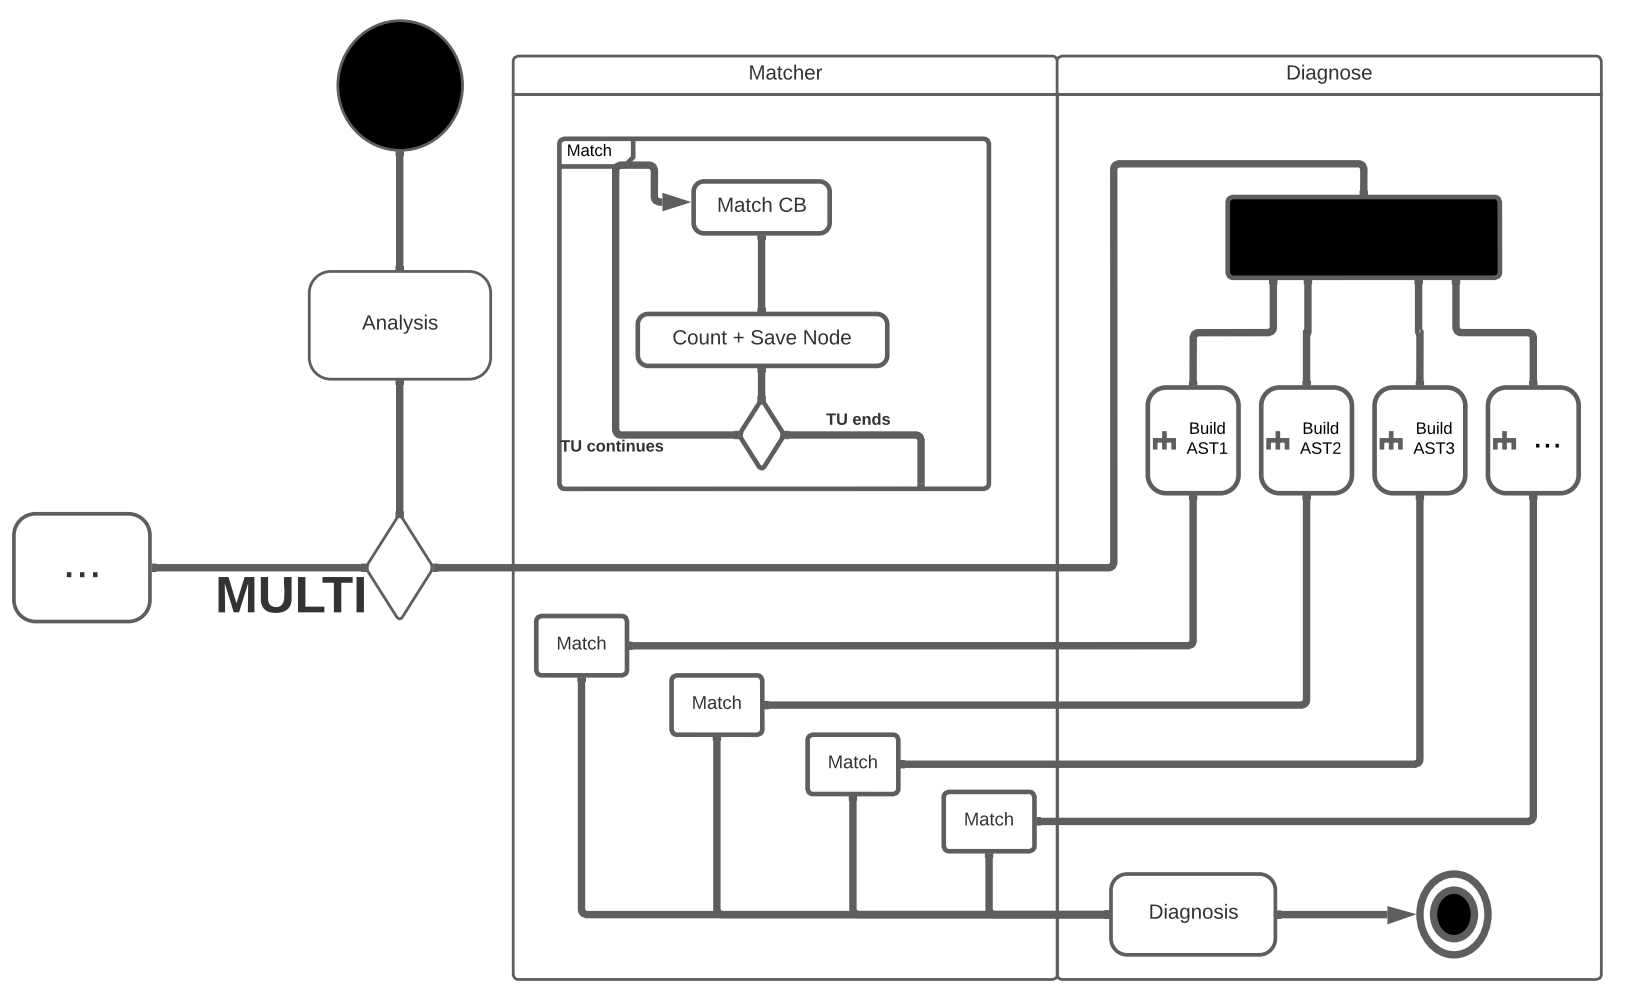
\includegraphics[width=\linewidth]{images/activity_single.png}
	\caption{Activity diagram of Clang-Tidy infrastructure in ``single'' mode.}
	\label{fig:activity-single}
\end{figure}

\begin{figure}[H]
	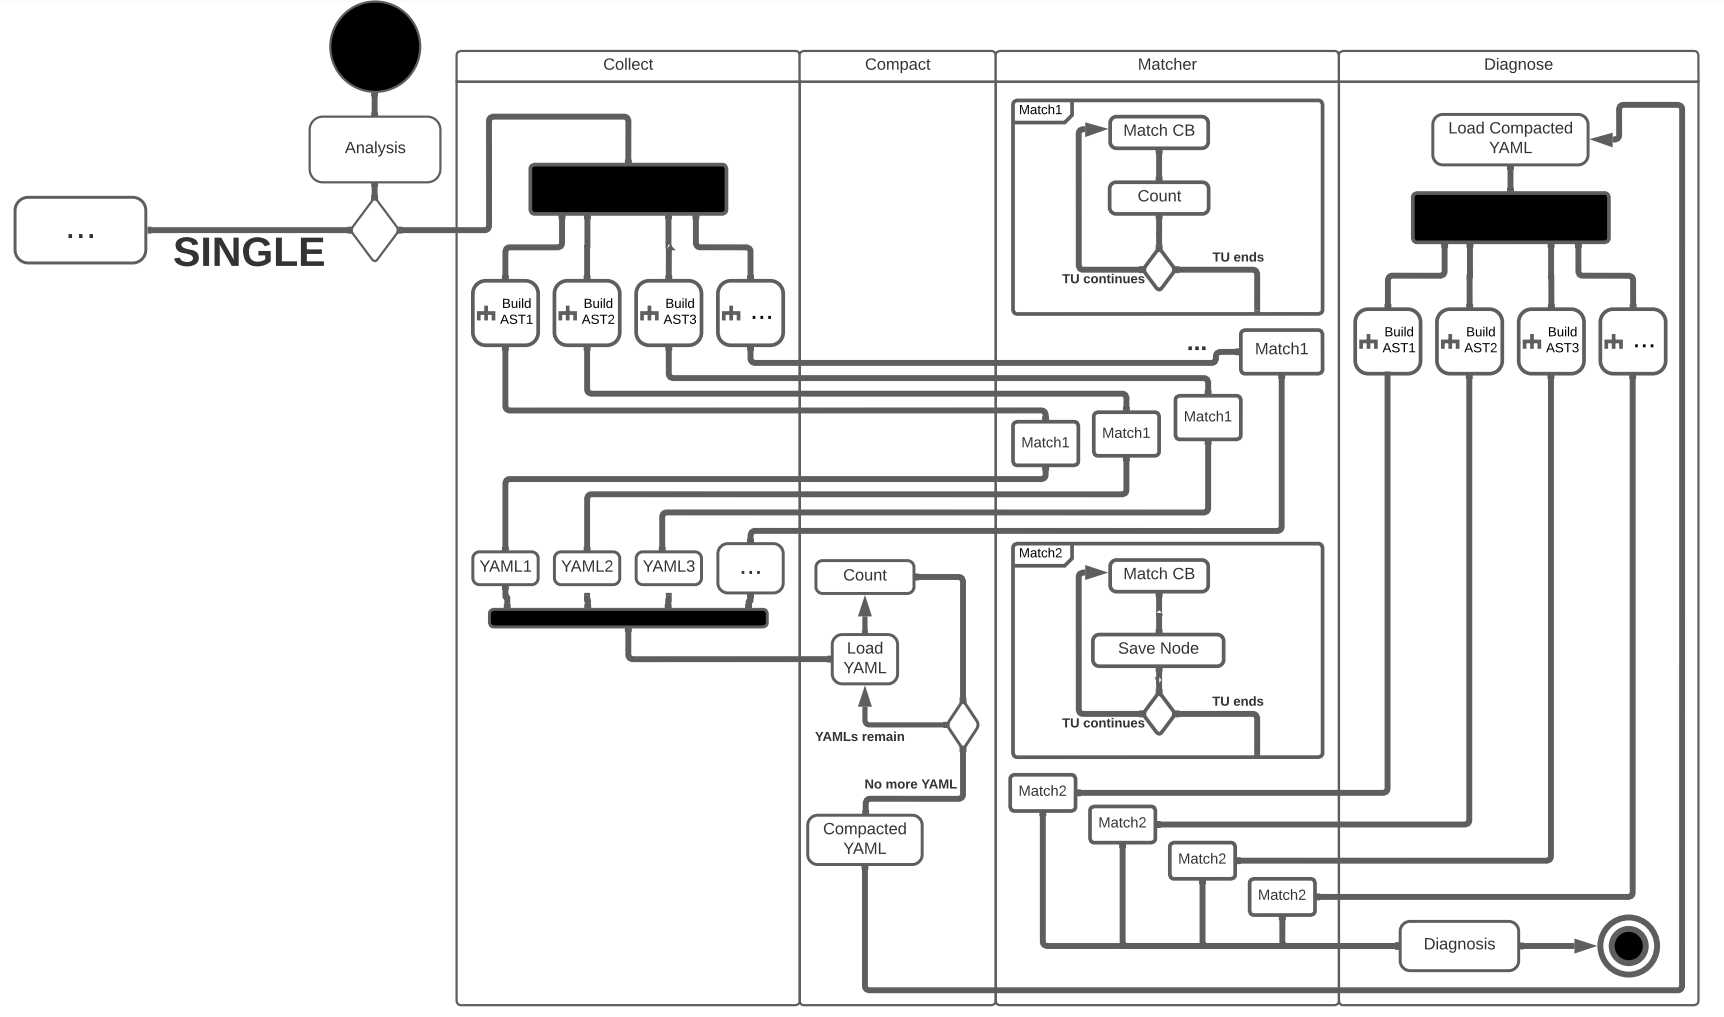
\includegraphics[width=\linewidth]{images/activity_multi.png}
	\caption{Activity diagram of Clang-Tidy infrastructure in ``multi'' mode.}
	\label{fig:activity-multi}
\end{figure}

The new flags I implemented are an \mintinline{CPP}{enum} flag for the current phase that we are in, and a regular \mintinline{CSharp}{string}
for the collection directory path. If the directory does not currently extist on the given path, the infrastructure will create one.

The base class of the checkers, \mintinline{CPP}{ClangTidyCheck} already has \mintinline{CPP}{virtual} functions for the checkers to override, with some
being optional and some not.
There are functions for \emph{language support}, registering \emph{preprocessor callbacks}, registering
\emph{matchers}, checking matched \emph{AST nodes}, and storing checker \emph{options}.
There are two additional functions from the base of
\mintinline{CPP}{ClangTidyCheck}, \mintinline{CPP}{MatchCallback}, and these are \mintinline{CPP}{onStartOfTranslationUnit} and \mintinline{CPP}{onEndOfTranslationUnit}, to
be able to do separate commands before and after the checker's actual work is done.

\begin{listing}[H]
  \begin{minted}{CPP}
/// Override this to register ``PPCallbacks`` in the preprocessor.
virtual void registerPPCallbacks(const SourceManager &SM,
  Preprocessor *PP,
  Preprocessor *ModuleExpanderPP) {}

/// Override this to register AST matchers with Finder.
virtual void registerMatchers(ast_matchers::MatchFinder *Finder) {}

/// ``ClangTidyChecks`` that register ASTMatchers should do the
/// actual work in here.
virtual void check(
  const ast_matchers::MatchFinder::MatchResult &Result) {}

/// Should store all options supported by this check with their
/// current values or default values for options that haven't been
/// overridden.
virtual void storeOptions(ClangTidyOptions::OptionMap &Options) {}
\end{minted}
\caption{Virtual functions from \mintinline{CPP}{ClangTidyCheck}'s header.}\label{lst:ctc-single-virtual}
\end{listing}

\begin{listing}[H]
\begin{minted}{CPP}
/// Called at the start of each translation unit.
/// Optionally override to do per translation unit tasks.
virtual void onStartOfTranslationUnit() {}

/// Called at the end of each translation unit.
/// Optionally override to do per translation unit tasks.
virtual void onEndOfTranslationUnit() {}
\end{minted}
\caption{Virtual functions from MatchCallback's header.}\label{lst:mc-single-virtual}
\end{listing}

Originally, when a \emph{callback} happened (which we will address later in \cref{sec:dev-checker})
\mintinline{CPP}{ClangTidyChecker} simply called the derived \mintinline{CPP}{class}'s \texttt{check} function.

\begin{listing}[H]
\begin{minted}{CPP}
void ClangTidyCheck::run(const MatchFinder::MatchResult &Result) {
	check(Result);
}
\end{minted}
\caption{The old infrastructure's way of calling \texttt{check}.}\label{lst:old-run}
\end{listing}

Now the checkers have three new \mintinline{CPP}{virtual void} member functions to override: \mintinline{CPP}{collect}, \mintinline{CPP}{postCollect}
and \texttt{compact}.
It is important to note that this override is optional, in a sense, that some checkers can not be improved with and do not need
project-level knowledge. If one, however, decides to use the new multipass infrastructure with one's checker, then none of these overrides
are optional.

\mintinline{CPP}{ClangTidyChecker} has a private \mintinline{CPP}{ClangTidyContext} member called \mintinline{CPP}{Context}.
This contains information about the current phase, the directory path and the
phase \mintinline{CPP}{enum} as well. This was used in the newly implemented member functions of the \mintinline{CPP}{ClangTidyChecker}
parent \mintinline{CPP}{class}, and with protected getter functions, the derived checker can use some information from this context.


As we can see in \cref{lst:old-run}, this function only called the checker's \mintinline{CPP}{check}, but now it distinguishes two
out of our 3 separate
phases, diagnose and collect. In diagnose phase, it still calls for \mintinline{CPP}{check}, but in collect phase it calls
for the checker's separate \texttt{collect} function.

\begin{listing}[H]
  \begin{minted}{CPP}
void ClangTidyCheck::run(const MatchFinder::MatchResult &Result) {
  switch (getPhase()) {
  case MultipassProjectPhase::Diagnose:
    check(Result);
    break;
  case MultipassProjectPhase::Collect:
    collect(Result);
    break;
  case MultipassProjectPhase::Compact:
    llvm_unreachable("AST Matchers should not have run in "
                     "compact mode.");
  }
}
  \end{minted}
  \caption{Run function distinguishing Diagnose and Collect phase.}\label{lst:new-run}
\end{listing}

After the collection has been done on a translation unit, the destructor of the \mintinline{CPP}{class} that
creates the checkers will call for the \mintinline{CPP}{runPostCollect} function of the base
\mintinline{CPP}{class}, which as the name suggests, runs the \mintinline{CPP}{postCollect} function of the derived checker.

During compact phase, the infrastructure does not need the translation units at all, so there are no checkers instantiated during the
compilation, since this phase excludes compilation. Instead, the checker creation is now refactored into a function and that is called
in a separate path of the code, where we only create the checkers and call compact on each of them once.

In the following subsections I will explain how the \mintinline{CPP}{virtual} functions should and how the member functions do work.

\subsection{Collect Function}

\mintinline{CPP}{collect} receives the same parameters as check does, a \mintinline{CPP}{MatchResult} reference. In this function the checker should
do something similar to its original check function. Usually, it gets information out of the translation unit, and stores it in a data
structure of choice that is fit for the checker's logic.

\subsection{PostCollect Function}

\mintinline{CPP}{postCollect} receives a \mintinline{CPP}{StringRef}, the name of the output YAML file. In this function a checker should take all the data
collected from the translation unit, from the data structure, and write it in a YAML file whose filename is the function parameter.

\subsection{Compact Function}

\mintinline{CPP}{compact} has two parameters. One is a \mintinline{CPP}{StringRef} that, similarly to \mintinline{CPP}{postCollect}, contains the
name of the output file.
The other is a \mintinline{CPP}{vector<string>}s that contains all the YAML files in our multipass directory, that the
current checker created in the collect phase and wrote the collection data into for each translation unit.
In this phase, the checker should collect all the data from these YAML files and compact them into a single data structure. After
this step, it should write it into the YAML file whose filename is the function parameter.

\subsection{Additional Functions}

There are newly implemented protected functions to use aside from these \mintinline{CPP}{virtual} ones:
\begin{itemize}
  \item \mintinline{CPP}{getCollectPath}: returns a \mintinline{CSharp}{string} to the path where the current check should write collected data to.
  \item \mintinline{CPP}{getCompactedDataPath}: returns a \mintinline{CPP}{StringRef}, the name of the file where the current check should write or read compacted data to/from.
  \item \mintinline{CPP}{getPhase}: returns the \mintinline{CPP}{enum} representing the current phase
\end{itemize}

\section{Discarded Return Value Check} % külön a checker részek meg az infrat használórészek pls
\label{sec:dev-checker}

In \cref{sec:prob-state}, we justified the existence of a checker which focuses on detecting potential bugs and code smells
and giving warnings to function calls where the return value is ignored or unchecked, if we deem it necessary by analysing the ratio
of the amount of unchecked calls and all calls for the same function.

\subsection{Abstract Syntax Trees}

Before making a checker, first we should know about how checkers work. Clang-Tidy checkers perform pattern matching on
Clang's object oriented and strong typed representation of the abstract syntax tree of the source code.
ASTs represent the syntactic structure of a code as seen in \cref{fig:ast1}.

In \cref{fig:ast1} we have 2 function declarations, one of which is our main. We can see that our other function is called \mintinline{CPP}{foo},
that takes no parameters and returns an \mintinline{CPP}{int}. In the \mintinline{CPP}{body} we have a statement, more specifically a
return statement. The subject of the return statement is a simple integer literal, with the value of 1.
In \texttt{main}, we only have another return statement, that has a call expression of a function that has a
declaration reference expression that refers to the declaration of our function \mintinline{CPP}{foo}.

Obviously, ASTs get increasingly more complex and harder to read as the source code grows. Another example can be seen on \cref{fig:ast2}.
\begin{figure}[H]
    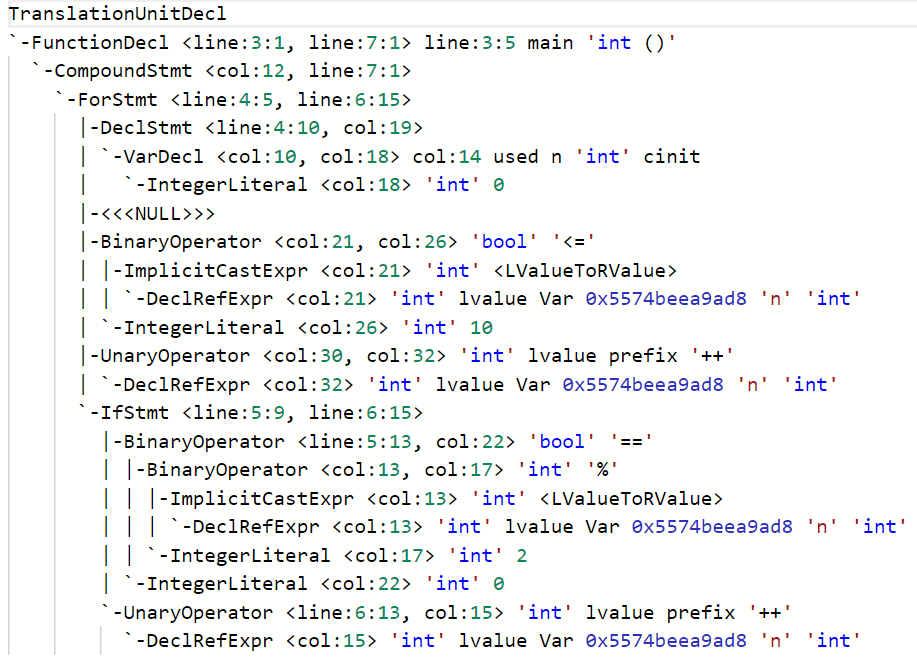
\includegraphics[width=\linewidth]{images/random_ast2.png}
	\caption{The AST of \cref{lst:ast2-code}}
    \label{fig:ast2}
\end{figure}

\begin{listing}[H]
  \begin{minted}{CPP}
int main() {
	for (int n = 0; n <= 10; ++n)
		if (n % 2 == 0)
			++n;
}
\end{minted}
\caption{The code of \cref{fig:ast2}.}\label{lst:ast2-code}
\end{listing}

\subsection{Pattern Matching}

Clang-Tidy checkers have \emph{matchers} that you can set up in the checker's overridden function \mintinline{CPP}{registerMatchers}.
This has its matcher, a \mintinline{CPP}{MatchFinder} as the parameter, and in this function we have to use its \mintinline{CPP}{addMatcher}
member function to add new patterns for it to match, and also to \mintinline{CPP}{bind} a string literal to the matches for later usage.
If the matcher finds a match, a \mintinline{CPP}{callback} action is executed.

In order to utilize the matches and the callbacks, we have to know how to match nodes on an AST. Clang-Tidy has built in matchers,
that we can see in the AST Matcher Reference~\cite{matcherref}. This tells us which matcher accepts which matcher or matchers as
parameter, and what their return type is. It also gives us examples of usage.
Theoretically, there are 3 distinct base types for AST nodes. \mintinline{CPP}{Decl} (declaration), \mintinline{CPP}{Stmt} (statement) and \mintinline{CPP}{Type}. In practice,
Clang-Tidy has more distinct bases in its AST representation, but for now let us view a simple example of matching from
\emph{Compiler Explorer}:\footnote{\url{http://godbolt.org/z/ncToe315q}, accessed 2022. 05. 14.}

\begin{listing}[H]
  \begin{minted}{CPP}
int foo() { return 1; }

int main() {
	foo();
	int n = foo();
	return foo();
}
  \end{minted}
  \caption{A very simple code for matching function calls.}\label{lst:matchercode}
\end{listing}

\begin{figure}[H]
    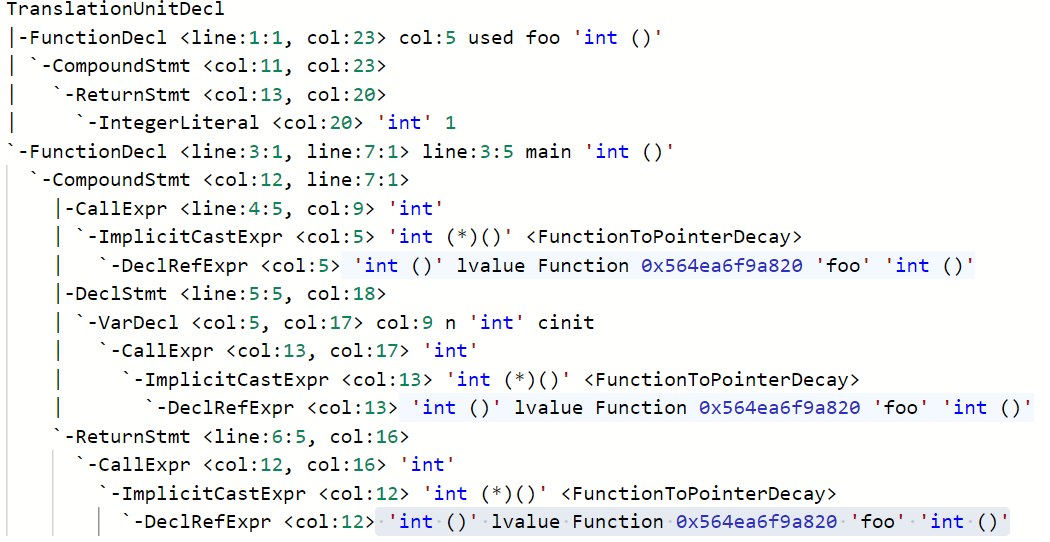
\includegraphics[width=\linewidth]{images/ast_for_matching.png}
	\caption{The AST of \cref{lst:matchercode}.}
    \label{fig:ast3}
\end{figure}

Here we can have 1 function declaration of the same function, and 3 call expressions, the first one in as a regular statement, the second one in
a variable declaration, and the third one in a return statement. Let us build a matcher for calls that a checker like mine should be
concerned about.
First, we want to match for function calls, whose declaration reference refers to a function declaration. If we use
\mintinline{CPP}{match callExpr(callee( declRefExpr(to(functionDecl().bind("definition"))) )).bind("call")} we get 3 matches
and 6 binds. It matches all 3 calls of \texttt{foo} bound to the literal \texttt{"call"}, and we also get 3 binds, all for the
first line, the \texttt{FunctionDecl} of \texttt{foo}, bound to \texttt{"definition"}.

We can also save the matcher bound to \texttt{"definition"} as a variable for easier usage and simplicity, if we wanted to.
With \mintinline{CPP}{let Def functionDecl().bind("definition")} it will be saved as \mintinline{CPP}{Def}, and with
\mintinline{CPP}{let Call callExpr(callee( declRefExpr(to(Def)) )).bind("call")}, where we reuse our \mintinline{CPP}{Def}, we save our \mintinline{CPP}{Call} for later use. Now we only have
to match for \mintinline{CPP}{Call} with \mintinline{CPP}{match Call} to get the same results.

We could improve it this matcher for the checker, with not matching functions declared with \mintinline{CPP}{void} as return value.
In Clang-Tidy the "saved" matcher will be a
\mintinline{CPP}{static const auto Call = callExpr(hasDeclaration(functionDecl(unless(returns(voidType())))));}. In reality, the
checker will need more specification in order to work properly, but this distinction is important as well.

There are separate matchers in static variables for any kind of usage of a return value, and then these are added in a single
\mintinline{CPP}{addMatcher} call of the matcher. Let us go through some of these matchers.

\subsubsection{Call}

Our actual specific call expression can be seen in \cref{lst:call}. Since this is the base of all other matchers
that we use, I will explain what we need to match for, in detail, starting with the bind. The \mintinline{CPP}{static constexpr} that \mintinline{CPP}{Call}
is bound to is an \mintinline{CPP}{llvm::StringLiteral} type, that wraps \texttt{"call"}.
We want to match for function calls, but not all function calls. First, we will sort out all functions whose declaration is a function
declaration to at least either a \mintinline{CPP}{void} function, because they do not return a value to be checked or ignored, and a
function with \mintinline{CPP}{[[nodiscard]]}, since the compiler will already warn the user if needed. This is what we achieve with lines
2-3. Second, we want to sort out any operator calls except for the following: \mintinline{CPP}{operator()} or \mintinline{CPP}{operator[]}
(this is done by lines 4-5), and \mintinline{CPP}{operator *} or \mintinline{CPP}{operator &}, but since those operators have multiple uses and
we want to include a specific use only, we only need these if they take only one argument, also known as the \emph{dereference}
and the \emph{address-of} operator (which is achieved by lines 6-7).
All of this specification can be seen in \cref{fig:venn-call}.


\begin{listing}[H]
  \begin{minted}{CPP}
static const auto Call =
	callExpr(hasDeclaration(functionDecl(unless(anyOf(
				 returns(voidType()), hasAttr(attr::WarnUnusedResult))))),
			 unless(cxxOperatorCallExpr(
				 unless(anyOf(hasAnyOverloadedOperatorName("()", "[]"),
							  allOf(hasAnyOverloadedOperatorName("*", "&"),
									argumentCountIs(1)))))))
		.bind(::Call);
  \end{minted}
  \caption{The matcher for our desired call expression.}\label{lst:call}
\end{listing}

\begin{figure}[H]
	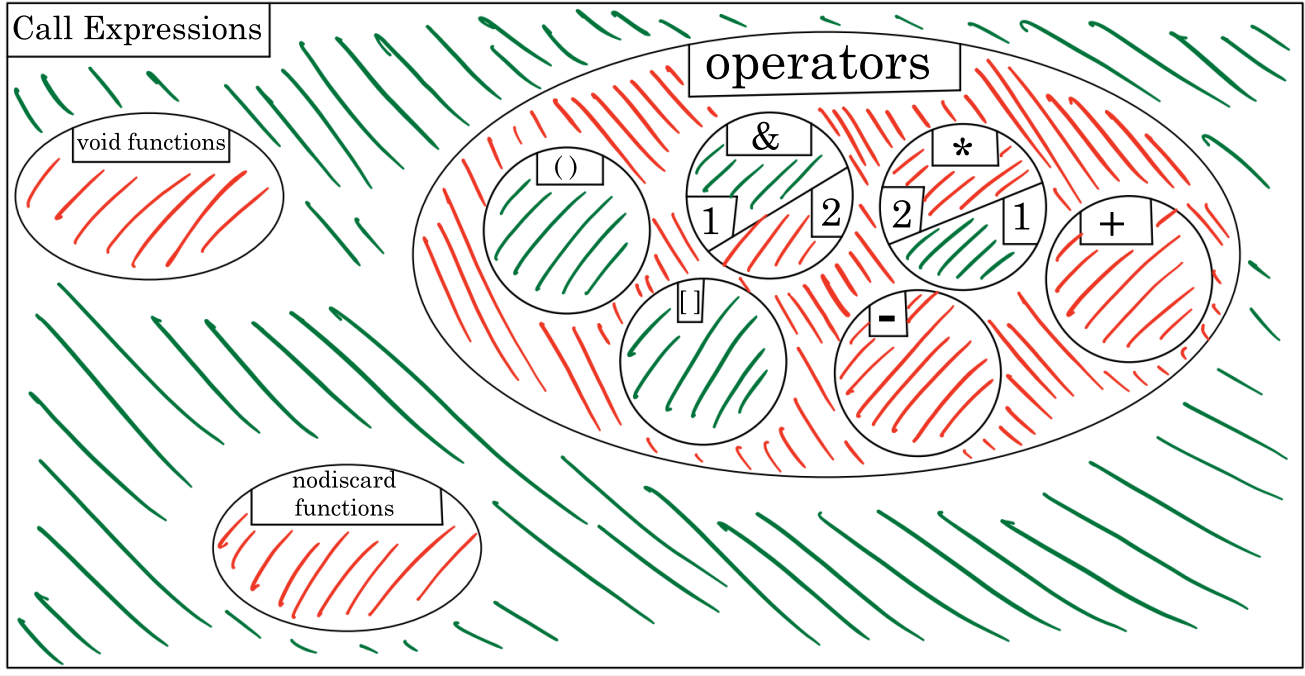
\includegraphics[width=\linewidth]{images/venn_call.png}
  \caption{A Venn-diagram of what \mintinline{CPP}{Call} (see \cref{lst:call}) matches, where 1 and 2 indicates the arity. The green subsets are to be matched.}
	\label{fig:venn-call}
\end{figure}

\subsubsection{While}

In \cref{lst:while} we match
for either a \texttt{while} statement or a \texttt{do} statement that uses our call in their condition, and then since the matcher
\mintinline{CPP}{anyOf} does not automatically cast its return type to that of a statement, we do it manually with \mintinline{CPP}{stmt}.

\begin{listing}[H]
  \begin{minted}{CPP}
static const auto While =
	stmt(anyOf(whileStmt(hasCondition(Call)),
             doStmt(hasCondition(Call))));
  \end{minted}
  \caption{The matcher for usage in while expression.}\label{lst:while}
\end{listing}

\subsubsection{Return}

In \cref{lst:return} we simply match if a return statement uses our function as its return value.

\begin{listing}[H]
  \begin{minted}{CPP}
static const auto Return = returnStmt(hasReturnValue(Call));
  \end{minted}
  \caption{The matcher for the usage in return statement.}\label{lst:return}
\end{listing} % TODO ide lehet törni kell a sort hogy ne legyen egyedül a caption az oldalon.

\subsubsection{For}

In \cref{lst:for} we match for
any and all of the following: if the \texttt{initialization}, the \texttt{condition}, or the \texttt{incrementation} of the for
loop, or if a \texttt{range-based} for loop, or any descendants of either of these uses the return value of our call.

\begin{listing}[H]
  \begin{minted}{CPP}
static const auto For = anyOf(
  forStmt(eachOf(hasLoopInit(findAll(Call)),
                 hasCondition(findAll(Call)),
                 hasIncrement(findAll(Call)))),
  cxxForRangeStmt(hasRangeInit(findAll(Call))));
  \end{minted}
  \caption{The matcher for the usage in for statement.}\label{lst:for}
\end{listing}

We can also create new matchers, should we need one that is not yet in the library. % ezt majd whispy átnézi
It provides \emph{\texttt{macros}} that can be used to implement matchers with custom logic. For example in \cref{lst:hasassert} the
macro defines a single-parameter function called \mintinline{CPP}{hasAssertExpr} that takes a \mintinline{CPP}{Matcher<Expr>} called
\mintinline{CPP}{InnerMatcher} and returns a \mintinline{CPP}{Matcher<StaticAssertDecl>} object. It passes the
matcher into the assertion expression of assert, meaning if the inner matcher matches, the entire assertion will too.

\begin{listing}[H]
  \begin{minted}{CPP}
AST_MATCHER_P(StaticAssertDecl, hasAssertExpr,
              ast_matchers::internal::Matcher<Expr>, InnerMatcher) {
  return InnerMatcher.matches(*Node.getAssertExpr(), Finder,
                              Builder);
}

static const auto StaticAssert =
    staticAssertDecl(hasAssertExpr(Call));
  \end{minted}
  \caption{Custom logic and usage of a new matcher called \mintinline{CPP}{hasAssertExpr}.}\label{lst:hasassert}
\end{listing}


\subsection{Checker Logic}

Before going into how my checker works, we should go through the member functions of it. The checker obviously overrides all
non-optional and some optional \mintinline{CPP}{virtual} functions as seen in \cref{lst:override-header}. In \cref{lst:drv-member}
there are three additional member functions. These contain the logic of the checker and how it shapes
its data structure according to the current phase. 

\begin{listing}[H]
  \begin{minted}{CPP}
void registerMatchers(ast_matchers::MatchFinder *Finder) override;
void storeOptions(ClangTidyOptions::OptionMap &Opts) override;
void onStartOfTranslationUnit() override;
void onEndOfTranslationUnit() override;
void collect(const ast_matchers::MatchFinder::MatchResult &Result)
  override;
void postCollect(StringRef OutputFile) override;
void compact(const std::vector<std::string> &PerTuCollectedData,
             StringRef OutputFile) override;
void check(const ast_matchers::MatchFinder::MatchResult &Result)
  override;
  \end{minted}
  \caption{Overridden virtual functions in \texttt{DiscardedReturnValueCheck}'s header.}\label{lst:override-header}
\end{listing}

\begin{listing}[H]
  \begin{minted}{CPP}
void matchResult(const MatchFinder::MatchResult &Result,
                 bool ShouldCount);
void registerCall(const CallExpr *CE, const FunctionDecl *FD,
                  bool IncrementCounters,
                  const void *ConsumingContext);
void diagnose(const Function &F);
  \end{minted}
  \caption{Private member functions in \texttt{DiscardedReturnValueCheck}'s header.}\label{lst:drv-member}
\end{listing}

For the data structure itself, The checker uses a \mintinline{CPP}{struct} representing the functions with their tracked amount of calls and
checks (and its member function calculating the ratio of these in percentage), a \mintinline{CPP}{StringMap} of functions to store their
name and their corresponding struct object, a \mintinline{CPP}{DenseMap} of \mintinline{CSharp}{FunctionDecl - String} pairs, a
\mintinline{CPP}{DenseMap} of \mintinline{CPP}{CallExpr - SmallVector} pairs to prevent multiple callbacks on a single call expression
being processed the twice. It also uses a \mintinline{Rust}{uint8_t} to save the threshold option, and an \mintinline{Rust}{Optional<bool>} to
track whether or not compacting has been done on the translation units.

\begin{listing}[H]
  \begin{minted}{CPP}
struct Function {
  std::size_t ConsumedCalls;
  std::size_t TotalCalls;
  const FunctionDecl *FD;
  llvm::SmallPtrSet<const CallExpr *, 32> DiscardedCEs;

  std::uint8_t ratio() const;
};
  using FunctionMapTy = llvm::StringMap<Function>;

  const std::uint8_t ConsumeThreshold;
  Optional<bool> CacheProjectDataLoadedSuccessfully;

  llvm::DenseMap<const CallExpr *, SmallVector<const void *, 2>>
      ConsumedCalls;
  llvm::DenseMap<const FunctionDecl *, std::string> FunctionIDs;
  FunctionMapTy CallMap;
  \end{minted}
  \caption{Members of the data structure.}\label{lst:remaining-members}
\end{listing}

After all the possible usages of a return value have been
refactored into these matchers, we put all of them into one call of \mintinline{CPP}{addMatcher} and bind them to
\mintinline{CPP}{"consume"}. In reality, the usages contain all 3 of the base node types, so we put these matchers into 3 \mintinline{CPP}{addMatcher} calls
in respect of which matcher returns which node type. The matchers \texttt{ExplicitCast}, \texttt{New}, \texttt{Delete}, \texttt{Argument}, \texttt{Unary}, \texttt{Dereference},
\texttt{BinaryLHS}, \texttt{BinaryRHS}, \texttt{If}, \texttt{While}, \texttt{For}, \texttt{Switch}, and \texttt{Return} should return statements; \texttt{StaticAssert}, \texttt{VarDecl}, and \texttt{CtorInits}
should return declarations; and \texttt{Decltype}, \texttt{TemplateArg}, and \texttt{VLA} should return types.
Now all we have to do is match for a simple call.

\begin{listing}[H]
  \begin{minted}{CPP}
  Finder->addMatcher(
	  traverse(
		  TK_IgnoreUnlessSpelledInSource,
		  stmt(eachOf(ExplicitCast, New, Delete, Argument, Unary,
					Dereference, BinaryLHS, BinaryRHS, If, While, For,
					Switch, Return)))
		  .bind(Consume),
	  this);
  Finder->addMatcher(traverse(TK_IgnoreUnlessSpelledInSource,
							  decl(eachOf(StaticAssert, VarDecl, CtorInits)))
					     .bind(Consume),
				     this);
  Finder->addMatcher(traverse(TK_IgnoreUnlessSpelledInSource,
							  type(eachOf(Decltype, TemplateArg, VLA)))
					     .bind(Consume),
				     this);

  Finder->addMatcher(traverse(TK_IgnoreUnlessSpelledInSource, Call),
                     this);
  \end{minted}
  \caption{Separating the matchers to statement, declaration, and type.}
\end{listing}

The checker will match for all function calls (that are not declared \mintinline{CPP}{void} et cetera) bound to \mintinline{CPP}{"call"}, and for the ones
that are checked it will match once more with the bind \mintinline{CPP}{"consume"}. For every match the callback happens and since matching \mintinline{CPP}{"consume"}
deterministically comes before matching \mintinline{CPP}{"call"}, we can be sure that if we matched with \mintinline{CPP}{"consume"} it is a checked call, and if we did
not, it is an unchecked call so we can count the checks of our matched call expressions accordingly. In \cref{lst:consume} we try to
get our \mintinline{CPP}{"consume"} bound node for either of the 3 base node types, and if either gets a node back, we count it as a checked return.
Otherwise we count it as unchecked.

\begin{listing}[H]
  \begin{minted}{CPP}
void DiscardedReturnValueCheck::matchResult(
	const MatchFinder::MatchResult &Result, bool ShouldCount) {
  const auto *CE = Result.Nodes.getNodeAs<CallExpr>(Call);
  assert(CE && "Bad matcher");

  const void *ConsumeNode = nullptr;
  if (const auto *D = Result.Nodes.getNodeAs<Decl>(Consume))
    ConsumeNode = D;
  if (const auto *S = Result.Nodes.getNodeAs<Stmt>(Consume))
    ConsumeNode = S;
  if (const auto *T = Result.Nodes.getNodeAs<Type>(Consume))
    ConsumeNode = T;
  if (ConsumeNode)
    return registerCall(CE, CE->getDirectCallee(), ShouldCount,
                        ConsumeNode);
  if (ConsumedCalls.find(CE) == ConsumedCalls.end())
    return registerCall(CE, CE->getDirectCallee(), ShouldCount,
                        nullptr);
}
  \end{minted}
  \caption{Catching nodes of used return values.}\label{lst:consume}
\end{listing}

Then the call expression is emplaced in our data structure for counting and because we do not want to count the same call twice, and if
the call belongs to a function declaration that have previously been saved in our data structure, then we also increment its data in
respect of it being checked or not.

At the end of the translation unit, we give our diagnostics.

\subsection{Multipass phases}

It is very clear that a checker like this is almost completely useless for projects larger than a single translation unit, unless we use
the enhanced infrastructure. This makes the checker a perfect fit to test it. First, we have to implement the new \mintinline{CPP}{virtual} functions.

\mintinline{CPP}{collect} does the same thing as the old \mintinline{CPP}{check} callback did. Because of this, the logic of this step was put
into a member function and is called in both functions, \mintinline{CPP}{check} and \mintinline{CPP}{collect}.

We save declarations and adjust the data structure with each new call of the same function. At the end of a translation unit, \mintinline{CPP}{postCollect}
writes this data into a new YAML file under the unique name that was generated by the infrastructure.

\mintinline{CPP}{compact} reads in all the data from the collection files, fills up the data structure and then it writes the compacted data into the output YAML.
Because both writing and reading into our data structure is necessary more than once in the checker, this also have been refactored, and \mintinline{CPP}{compact},
\mintinline{CPP}{postCollect} and \mintinline{CPP}{check} all call these functions.

In \cref{lst:load}, we can see that we first extract the data from the YAML file into an optional \mintinline{CPP}{vector} of the function representation,
and if the extraction actually happened, we emplace and modify the data of the files into the current state of the data structure. At the end, it returns
whether succesful extraction happened or not.
In \cref{lst:write} we see that \mintinline{CPP}{writeYAML} puts our data into the output \mintinline{CPP}{stream}.
These are both examples of possible writing and loading methods for YAML serialization that are easy to use and implement using LLVM's YAML library~\cite{yamllib}.

\begin{listing}[H]
  \begin{minted}{CPP}
using FunctionVec = std::vector<SerializedFunction>;

static Optional<FunctionVec> loadYAML(StringRef File) {
  using namespace llvm;

  ErrorOr<std::unique_ptr<MemoryBuffer>> IStream =
  	MemoryBuffer::getFileAsStream(File);
  if (!IStream)
    return None;

  FunctionVec R;
  yaml::Input YIn{**IStream};
  YIn >> R;

  return R;
}

static bool loadYAML(StringRef FromFile,
					   DiscardedReturnValueCheck::FunctionMapTy &ToMap) {
  Optional<FunctionVec> OV = loadYAML(FromFile);
  if (!OV)
    return false;

  for (const SerializedFunction &SF : *OV) {
    DiscardedReturnValueCheck::Function &F =
      ToMap
    	  .try_emplace(SF.ID,
    				DiscardedReturnValueCheck::Function{0, 0, nullptr, {}})
    	  .first->second;

    F.ConsumedCalls += SF.ConsumedCalls;
    F.TotalCalls += SF.TotalCalls;
  }

  return true;
}
  \end{minted}
  \caption{Functions for loading.}\label{lst:load}
\end{listing}

\begin{listing}[H]
  \begin{minted}{CPP}
static void writeYAML(StringRef Whence, FunctionVec Elements,
                      StringRef ToFile) {
  std::error_code EC;
  llvm::raw_fd_ostream FS(ToFile, EC, llvm::sys::fs::OF_Text);
  if (EC) {
    llvm::errs() << "DiscardedReturnValueCheck: Failed to write "
                 << Whence << " output file: " << EC.message();
    llvm::report_fatal_error("", false);
    return;
  }

  llvm::yaml::Output YAMLOut(FS);
  YAMLOut << Elements;
}
  \end{minted}
  \caption{Function for writing.}\label{lst:write}
\end{listing}

Both \mintinline{CPP}{postCollect} and \mintinline{CPP}{compact} uses \mintinline{CPP}{writeYAML} with the YAML compatible representation of the function representation. For the
purpose of writing, these functions both use a refactored function that converts the latter into the YAML compatible version. These are seen in
\cref{lst:yamlize} with the method of making a \mintinline{CPP}{struct} YAML compatible as well.

\begin{listing}[H]
  \begin{minted}{CPP}
struct SerializedFunction {
  std::string ID;
  std::size_t ConsumedCalls, TotalCalls;
};

template <> struct MappingTraits<SerializedFunction> {
  static void mapping(IO &IO, SerializedFunction &F) {
    IO.mapRequired("ID", F.ID);
    IO.mapRequired("Consumed", F.ConsumedCalls);
    IO.mapRequired("Total", F.TotalCalls);
  }
};

LLVM_YAML_IS_SEQUENCE_VECTOR(SerializedFunction)

static FunctionVec
yamlize(const DiscardedReturnValueCheck::FunctionMapTy &Map) {
  FunctionVec SFs;
  llvm::transform(Map, std::back_inserter(SFs), [](auto &&E) {
    return SerializedFunction{E.first().str(),
                              E.second.ConsumedCalls,
                              E.second.TotalCalls};
  });
  return SFs;
}
  \end{minted}
  \caption{Steps for making the data YAML writable.}\label{lst:yamlize}
\end{listing}

Check works in a similar way. First, we check if compact has happened already. If not, check runs without project-level knowledge and emits diagnostics
per translation unit, the same
way as before. If compact phase has not been run for this checker, we fill up our data structure, but only if this step has not happened before.
For this, we use the same refactored functions as in \mintinline{CPP}{collect}, \mintinline{CPP}{matchResult} and thus \mintinline{CPP}{registerCalls}, with the exception
that adjustments in the data structure after each call does not need to happen, since all the data on the amount of checks and calls had been acquired before,
from the compacted file. Then we take the unique name (as a \mintinline{CSharp}{string}) of a function
declaration, or generate one if one does not already exist. After this we check again, whether or not we stored this declaration in the data structure,
and if not, we store it, but only if its call was unused, and then if compact has not happened, we increment its data accordingly. If it
has, we have nothing left to do. Now we only need to emit diagnostics to the right calls, which happens at the end of each translation unit.

\section{Evaluation}
\label{sec:eval}

This checker's upgrade to the multipass infrastructure differs from the original one only by a little. However,
it gives us very different results. The checker has run on large projects. It ran with 50\% and 80\% threshold both with and
without collection and compacting. The results are shown in \cref{tab:proj-test}

\pagebreak
%\begin{center}
	\begin{longtable}{ | m{0.35\textwidth} | m{0.2\textwidth} | m{0.14\textwidth} | m{0.18\textwidth} | } % jobbra a számok és ezres , \,
		
		\hline
		\textbf{Project name} & \textbf{Multi-pass?} & \textbf{Threshold} & \textbf{\# reports}  \\
		\hline \hline
		\endfirsthead
		
		\hline
		\textbf{Project name} & \textbf{Multi-pass?} & \textbf{Threshold} & \textbf{\# reports}  \\
		\hline \hline
		\endhead

		\hline
		\endfoot
		\endlastfoot

		\multirow{4}{*}{Bitcoin \texttt{v0.20.1}~\cite{bitcoin}}
		& \ding{53} & \hfill{}50\% & \hfill{}140 \\
		& \ding{51} & \hfill{}50\% & \hfill{}320 \\
		& \ding{53} & \hfill{}80\% & \hfill{}25 \\
		& \ding{51} & \hfill{}80\% & \hfill{}92 \\
		\hline

		\multirow{4}{*}{CodeChecker \texttt{v6.17.0}~\cite{codechecker}}
		& \ding{53} & \hfill{}50\% & \hfill{}2 \\
		& \ding{51} & \hfill{}50\% & \hfill{}5 \\
		& \ding{53} & \hfill{}80\% & \hfill{}0 \\
		 & \ding{51} & \hfill{}80\% & \hfill{}0 \\
		\hline

		\multirow{4}{*}{Contour \texttt{v0.2.0.173}~\cite{contour}}
		& \ding{53} & \hfill{}50\% & \hfill{}38 \\
		& \ding{51} & \hfill{}50\% & \hfill{}107 \\
		& \ding{53} & \hfill{}80\% & \hfill{}10 \\
		 & \ding{51} & \hfill{}80\% & \hfill{}8 \\
		\hline

		\multirow{4}{*}{cURL \texttt{7.66.0}~\cite{curl}}
		& \ding{53} & \hfill{}50\% & \hfill{}55 \\
		& \ding{51} & \hfill{}50\% & \hfill{}210 \\
		& \ding{53} & \hfill{}80\% & \hfill{}6 \\
		 & \ding{51} & \hfill{}80\% & \hfill{}104 \\
		\hline

		\multirow{4}{*}{FFmpeg \texttt{n4.3.1}~\cite{ffmpeg}}
		& \ding{53} & \hfill{}50\% & \hfill{}904 \\
		& \ding{51} & \hfill{}50\% & \hfill{}1\,846 \\
		& \ding{53} & \hfill{}80\% & \hfill{}148 \\
		 & \ding{51} & \hfill{}80\% & \hfill{}613 \\
		 \hline

		 \multirow{4}{*}{libWebM \texttt{1.0.0.27}~\cite{libwebm}}
		 & \ding{53} & \hfill{}50\% & \hfill{}9 \\
		 & \ding{51} & \hfill{}50\% & \hfill{}10 \\
		 & \ding{53} & \hfill{}80\% & \hfill{}0 \\
		 & \ding{51} & \hfill{}80\% & \hfill{}1 \\
		 \hline

		 \multirow{4}{*}{LLVM \texttt{12.0.0}~\cite{llvm}}
		 & \ding{53} & \hfill{}50\% & \hfill{}4\,615 \\
		 & \ding{51} & \hfill{}50\% & \hfill{}6\,837 \\
		 & \ding{53} & \hfill{}80\% & \hfill{}1\,077 \\
		  & \ding{51} & \hfill{}80\% & \hfill{}2\,150 \\
		 \hline

		 \multirow{4}{*}{Memcached \texttt{1.6.8}~\cite{memcached}}
		 & \ding{53} & \hfill{}50\% & \hfill{}32 \\
		 & \ding{51} & \hfill{}50\% & \hfill{}49 \\
		 & \ding{53} & \hfill{}80\% & \hfill{}5 \\
		  & \ding{51} & \hfill{}80\% & \hfill{}16 \\
		 \hline

		 \multirow{4}{*}{MongoDB \texttt{r4.4.6}~\cite{mongo}}
		 & \ding{53} & \hfill{}50\% & \hfill{}1\,671 \\
		 & \ding{51} & \hfill{}50\% & \hfill{}2\,463 \\
		 & \ding{53} & \hfill{}80\% & \hfill{}370 \\
		  & \ding{51} & \hfill{}80\% & \hfill{}1\,223 \\
		  \hline

		 \multirow{4}{*}{OpenSSL \texttt{3.0.0}~\cite{openssl}}
		 & \ding{53} & \hfill{}50\% & \hfill{}427 \\
		 & \ding{51} & \hfill{}50\% & \hfill{}1\,060 \\
		 & \ding{53} & \hfill{}80\% & \hfill{}56 \\
		  & \ding{51} & \hfill{}80\% & \hfill{}244 \\
		 \hline

		\multirow{4}{*}{PostgreSQL \texttt{r13.0}~\cite{postgres}}
		& \ding{53} & \hfill{}50\% & \hfill{}799 \\
		& \ding{51} & \hfill{}50\% & \hfill{}644 \\
		& \ding{53} & \hfill{}80\% & \hfill{}62 \\
		 & \ding{51} & \hfill{}80\% & \hfill{}215 \\
		\hline

		\multirow{4}{*}{Protocol Buffers \texttt{v3.13.0}~\cite{protobuf}}
		& \ding{53} & \hfill{}50\% & \hfill{}51 \\
		& \ding{51} & \hfill{}50\% & \hfill{}122 \\
		& \ding{53} & \hfill{}80\% & \hfill{}20 \\
		 & \ding{51} & \hfill{}80\% & \hfill{}75 \\
		\hline

		\multirow{4}{*}{Qt Base \texttt{v6.2.0}~\cite{qtbase}}
		& \ding{53} & \hfill{}50\% & \hfill{}1\,195 \\
		& \ding{51} & \hfill{}50\% & \hfill{}2\,764 \\
		& \ding{53} & \hfill{}80\% & \hfill{}200 \\
		 & \ding{51} & \hfill{}80\% & \hfill{}1\,093 \\
		\hline

		\multirow{4}{*}{SQLite \texttt{3.33.0}~\cite{sqlite}}
		& \ding{53} & \hfill{}50\% & \hfill{}284 \\
		& \ding{51} & \hfill{}50\% & \hfill{}288 \\
		& \ding{53} & \hfill{}80\% & \hfill{}42 \\
		 & \ding{51} & \hfill{}80\% & \hfill{}48 \\
		\hline

		\multirow{4}{*}{tmux \texttt{2.6}~\cite{tmux}}
		& \ding{53} & \hfill{}50\% & \hfill{}35 \\
		& \ding{51} & \hfill{}50\% & \hfill{}48 \\
		& \ding{53} & \hfill{}80\% & \hfill{}1 \\
		 & \ding{51} & \hfill{}80\% & \hfill{}1 \\
		\hline

		\multirow{4}{*}{twin \texttt{v0.8.1}~\cite{twin}}
		& \ding{53} & \hfill{}50\% & \hfill{}54 \\
		& \ding{51} & \hfill{}50\% & \hfill{}69 \\
		& \ding{53} & \hfill{}80\% & \hfill{}9 \\
		 & \ding{51} & \hfill{}80\% & \hfill{}22 \\
		\hline

		\multirow{4}{*}{Vim \texttt{v8.2.1920}~\cite{vim}}
		& \ding{53} & \hfill{}50\% & \hfill{}227 \\
		& \ding{51} & \hfill{}50\% & \hfill{}383 \\
		& \ding{53} & \hfill{}80\% & \hfill{}32 \\
		 & \ding{51} & \hfill{}80\% & \hfill{}54 \\
		\hline

		\multirow{4}{*}{Xerces \texttt{v3.2.3}~\cite{xerces}}
		& \ding{53} & \hfill{}50\% & \hfill{}125 \\
		& \ding{51} & \hfill{}50\% & \hfill{}197 \\
		& \ding{53} & \hfill{}80\% & \hfill{}9 \\
		 & \ding{51} & \hfill{}80\% & \hfill{}38 \\
		\hline

		\caption{Results of different runs on live projects.} \label{tab:proj-test}
	\end{longtable}
%\end{center}

In \cref{tab:proj-test}, we can see that the numbers between both single and multiple phase, and 50\% and 80\% threshold runs largely differ
in a considerable amount of test projects. There were results where the multiple phase run gave more warnings, indicating the aforementioned
bugs hiding in separate translation units only, and some results where it gave less warnings, indicating false positives in single runs.

In \cref{fig:ff-80-single} and \cref{fig:ff-80-multi}, we can see diagrams of the results. Each line represents a function, with
its height as the total amount of calls. The green and red parts represent the checked and unchecked calls, respectively. The descending graph of black
dots display the ratio of checked to all calls, which is important regarding our threshold.

In these runs, the amount of separate unchecked functions were similar, but using the multi-pass infrastructure, the amount of calls for these functions was
obviously a lot higher. In the old infrastructure run, the ratios are closer to the 80\% threshold, and most functions here were called less than 20
times, and were only unchecked once or twice. However, if we look at the multi-pass run, the ratios are a lot higher. They were unchecked only
a couple of times in this run as well, but the amount of total calls per function was bigger than in the previous run, resulting in the
functions staying more consistently above our 80\% threshold.

\begin{figure}[H]
	\makebox[\textwidth]{\includegraphics[width=1.2\linewidth]{images/FFmpeg_80_1_Single.png}}
	\caption{Diagram of 80\% threshold single run on FFmpeg.}
	\label{fig:ff-80-single}
\end{figure}

\begin{figure}[H]
	\makebox[\textwidth]{\includegraphics[width=1.2\linewidth]{images/FFmpeg_80_2_Multi.png}}
	\caption{Diagram of 80\% threshold multi run on FFmpeg.}
	\label{fig:ff-80-multi}
\end{figure}

Let us take a look at a 50\% threshold run comparison as well. In \cref{fig:bc-50-single} and \cref{fig:bc-50-multi} we get very different
results again. Here we can still see the higher ratios in the multi run, as well as higher overall amount of function calls. This time we
have more unchecked calls for functions that have been called considerably more than the rest, in both amount and ratio.

\begin{figure}[H]
	\makebox[\textwidth][c]{\includegraphics[width=1.2\linewidth]{images/Bitcoin_50_1_Single.png}}
	\caption{Diagram of 50\% threshold single run on Bitcoin.}
	\label{fig:bc-50-single}
\end{figure}

\begin{figure}[H]
	\makebox[\textwidth][c]{\includegraphics[width=1.2\linewidth]{images/Bitcoin_50_2_Multi.png}}
	\caption{Diagram of 50\% threshold multi run on Bitcoin.}
	\label{fig:bc-50-multi}
\end{figure}

The diagrams for all of the aforementioned project tests can be found in \cref{appx:diagrams}.
What can be said about almost all of the larger results is that they have a great amount of functions barely passing the threshold whose total
amount of calls do not exceed a considerable number compared to the size of the project and some other functions within the results. These could
potentially be ignored in some cases in the future.


\cleardoublepage

\chapter{Conclusion}
\label{ch:sum}

This thesis demonstrated the problem of unchecked return values, to which problem it gave a solution in form of a statistical method without
actually modifying the source code of said unchecked return values. This solution was made as an implementation in the Clang-Tidy pattern
matching based static analysis library, however the statistical method would fail because of the way Clang-Tidy checkers work, separately
for each translation unit. This leads to invalid statistics. In order to fix this, I have enhanched the infrastructure and created the
option of multiphase analysis, that will collect the needed information per translation unit, accumulate these and make a project-level set
of information, and finally emit diagnosis with this newly compacted information. The finished checker was accomplished using this new
infrastructure. This checker method can obviously run without the use of multiphase analysis, because the new infrastructure is made to be
backwards compatible with the single phase mode, but the new infrastructure was vital for the statistics of the checker. This proved the
checker to be an excellent example for the usage and utility of the multiphase mode.

\section{Future Work}

Previously in \cref{sec:eval}, I talked about ignoring a set of functions whose total amount of calls do not exceed a given value. This could
potentially be implemented into the checker as an option, so that the user could give the checker the number, and the checker will not give
warnings to a function call if the function's amount of calls is less than said number. It would make the results clearer in some cases.

The first possible future work ignores functions based on their statistics, but ignoring based on function property could be useful too.
The checker should categorically ignore some functions. There are also functions whose return value can not always be checked. A classic
example would be the \lstinline{<<} operator or \lstinline{std::append}, since the first will always return the \texttt{stream}, and the latter
will always return \lstinline{*this} for continuous use of the same function. \lstinline{std::cout << '1 ' << '2 ' << '3' << std::endl;} will
always be unchecked in the end, since the last \lstinline{<<} can not be checked with merit and without creating another unchecked return value.

The hash generation for the YAML filename does not respect multiple compilations of the same file with different compile flags. This is something
that could be fixed in the future as well.

\section*{Acknowledgements}

I would like to express my deepest appreciation to my supervisor, Richárd Szalay for his invaluable patience and feedback, and without whom
I could not have completed this thesis in time. I am also greatful to my professor, Dr. Zoltán Porkoláb, who generously provided his knowledge,
expertise and inspiration. Furthermore I would highlight Aaron Ballman's (Intel Corporation) and Gábor Márton's (Ericsson AB.) insights during
the open-source code review process.
\cleardoublepage

% Appendices (optional) - useful for detailed information in long tables, many and/or large figures, etc.
\appendix
\chapter{Project results}
\label{appx:diagrams}

The Discarded Return Value Checker was run on 18 different live project with 4 different setting. Two using the new
multiple phase infrastructure and two with the single phase one, on 50\% treshold and on 80\% treshold. These are
the results of the runs regarding the amount of different functions found, their amount of calls both checked and unchecked,
and the ratio of these two amounts.
\pagebreak

\begin{figure}[H]
	\makebox[\textwidth]{\includegraphics[width=1.2\linewidth]{images/appendix/Bitcoin_50_1_Single.png}}
\end{figure}

\begin{figure}[H]
	\makebox[\textwidth]{\includegraphics[width=1.2\linewidth]{images/appendix/Bitcoin_50_2_Multi.png}}
\end{figure}

\begin{figure}[H]
	\makebox[\textwidth]{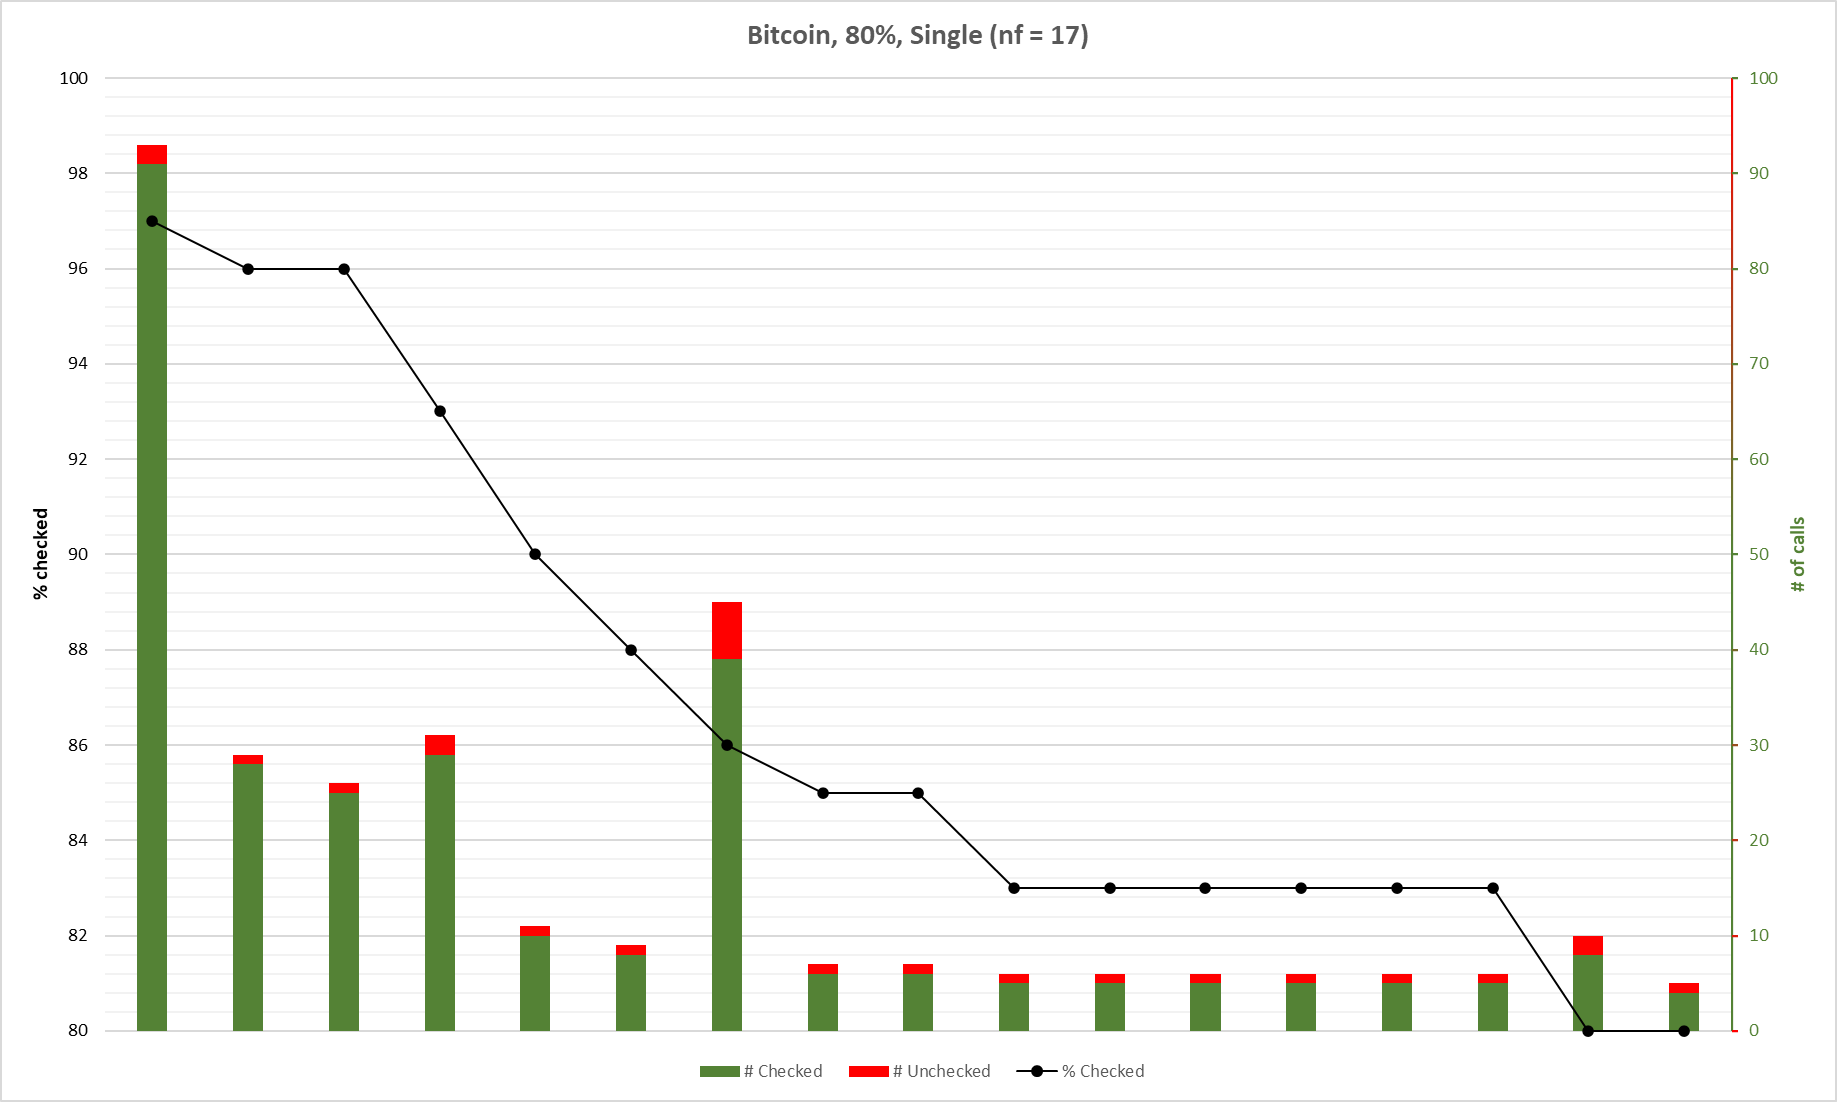
\includegraphics[width=1.2\linewidth]{images/appendix/Bitcoin_80_1_Single.png}}
\end{figure}

\begin{figure}[H]
	\makebox[\textwidth]{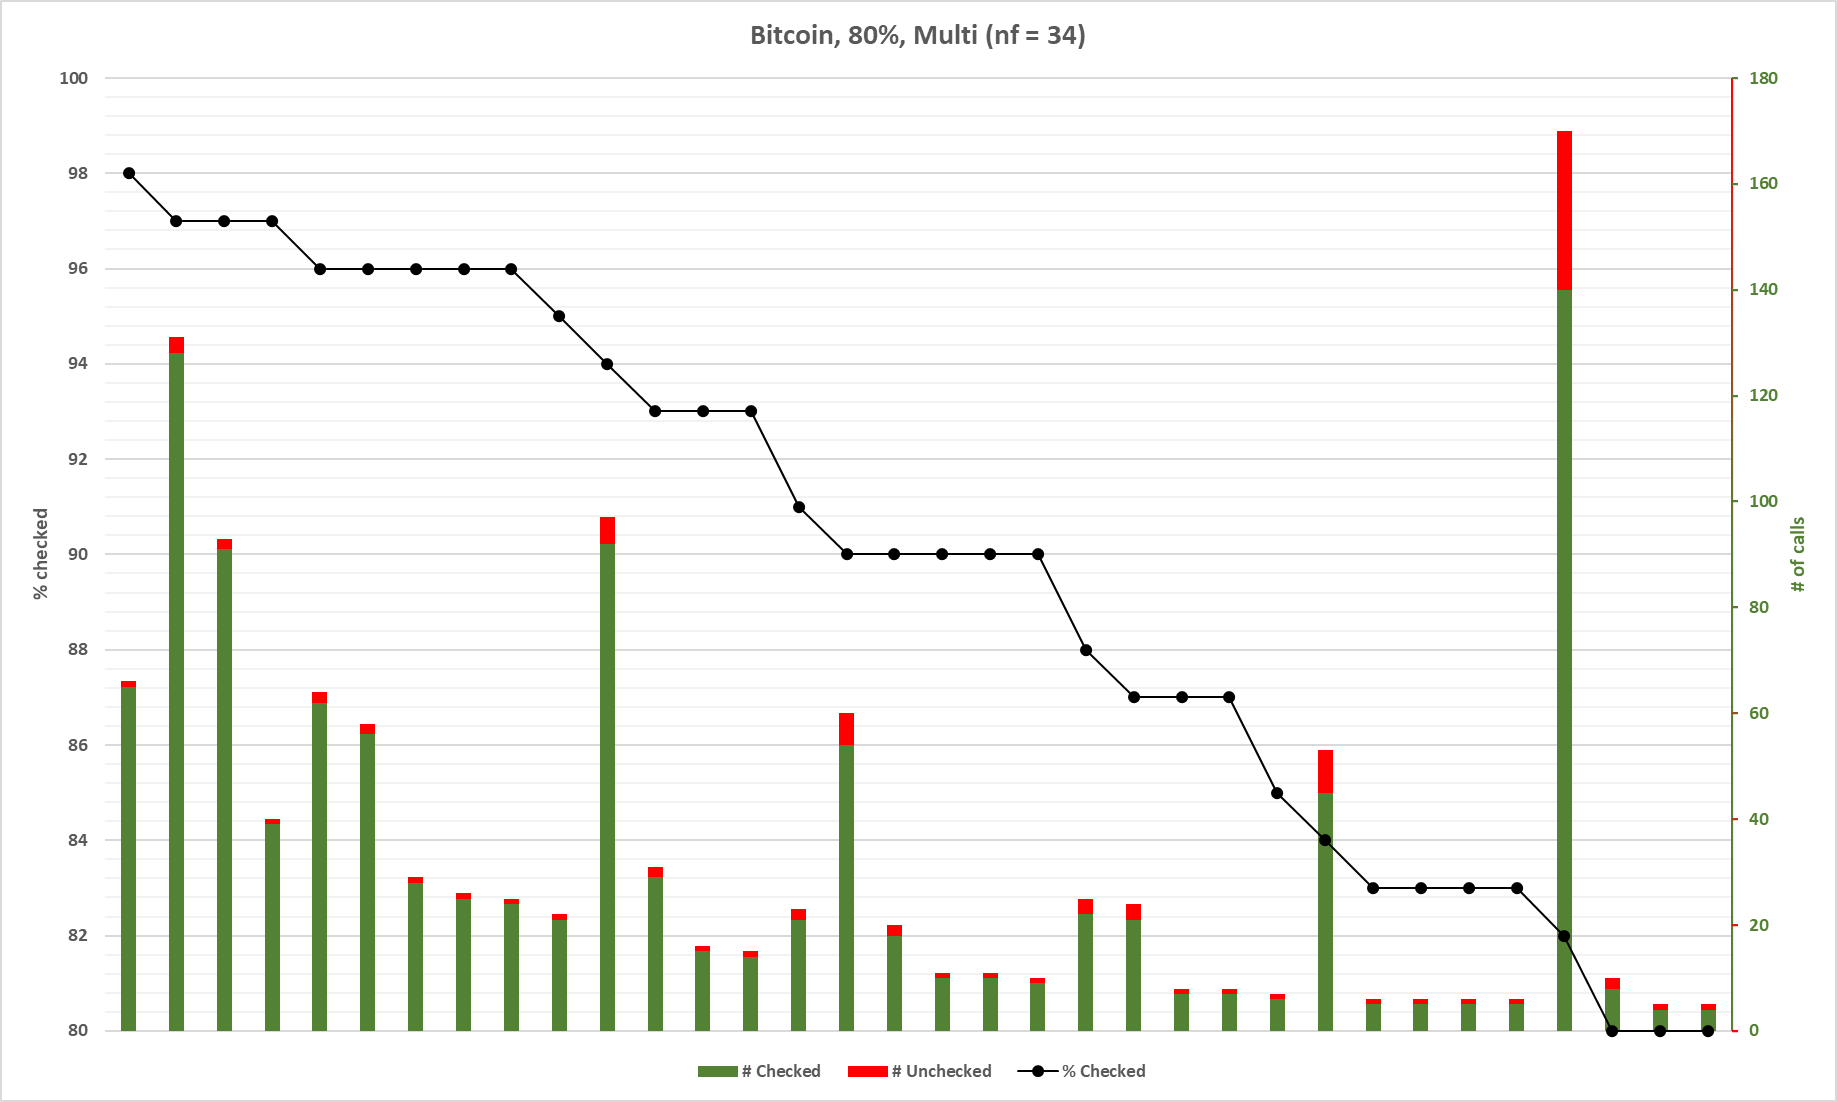
\includegraphics[width=1.2\linewidth]{images/appendix/Bitcoin_80_2_Multi.png}}
\end{figure}

\begin{figure}[H]
	\makebox[\textwidth]{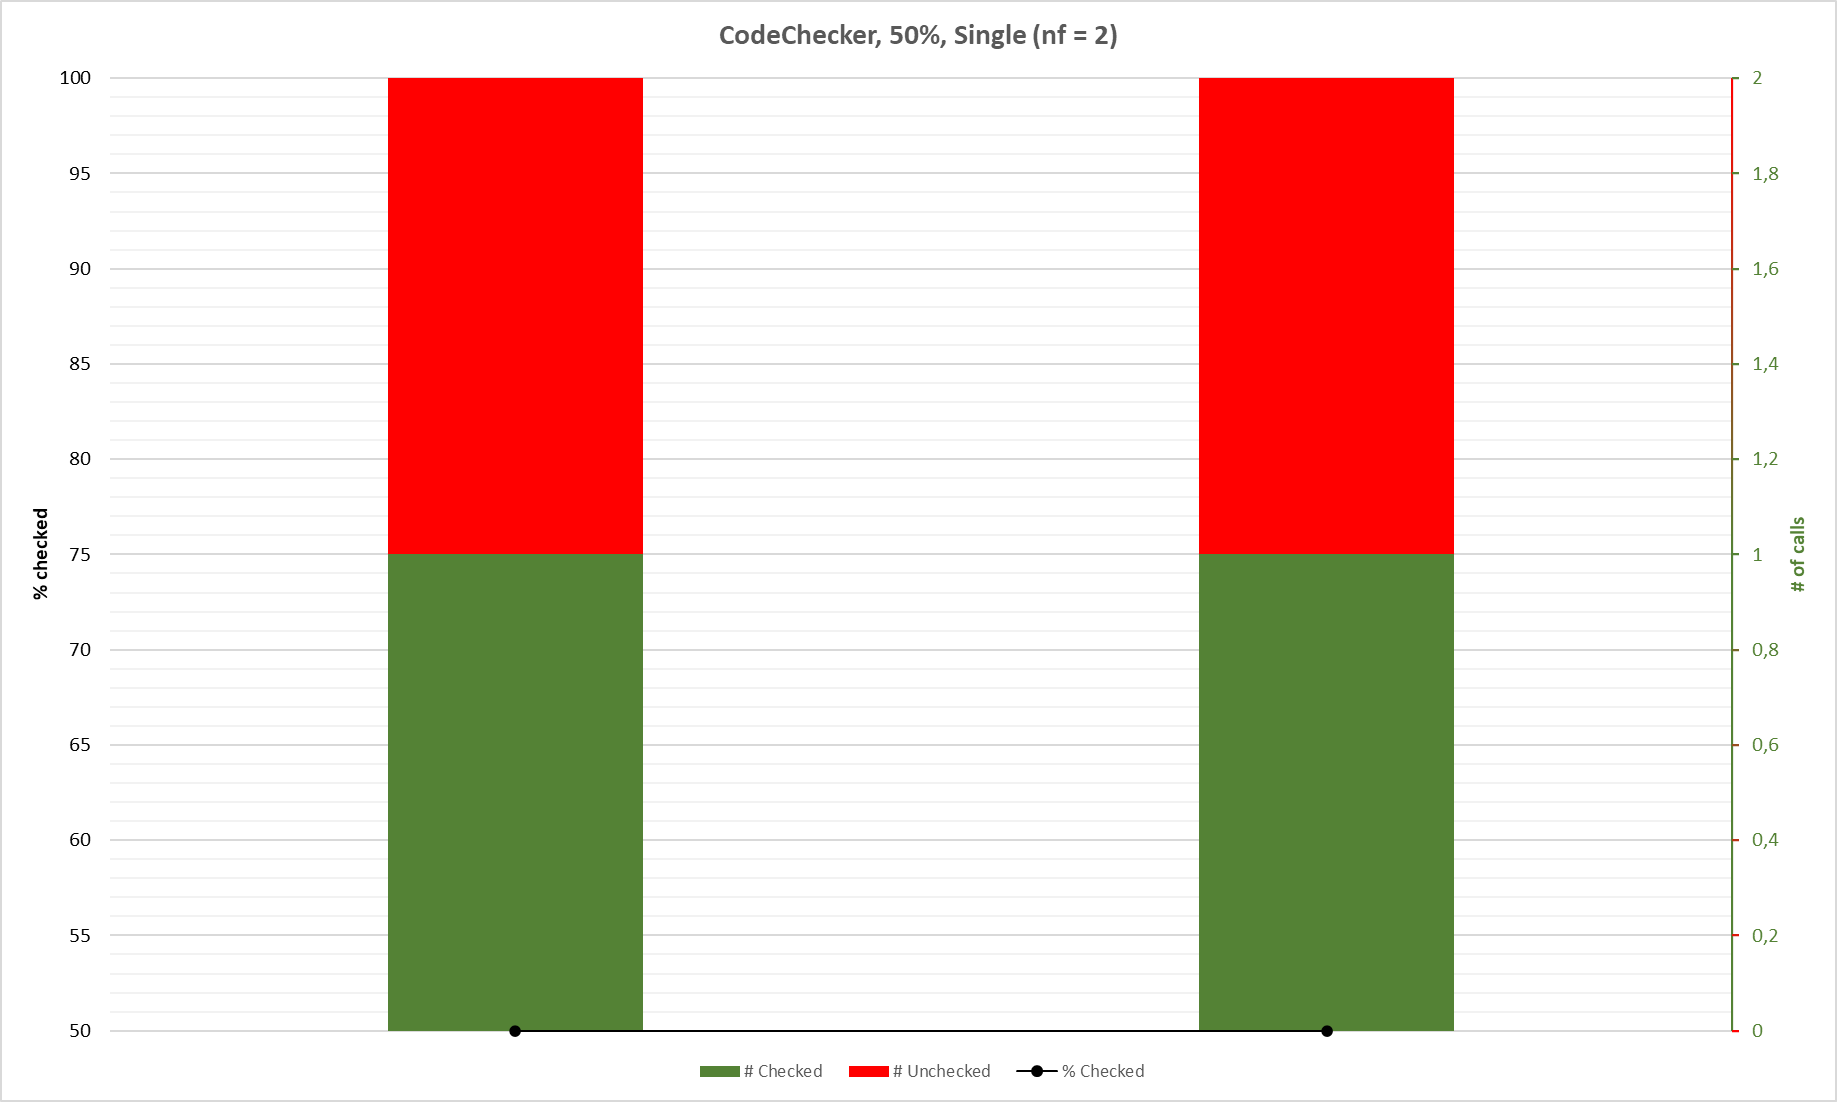
\includegraphics[width=1.2\linewidth]{images/appendix/CodeChecker_50_1_Single.png}}
\end{figure}

\begin{figure}[H]
	\makebox[\textwidth]{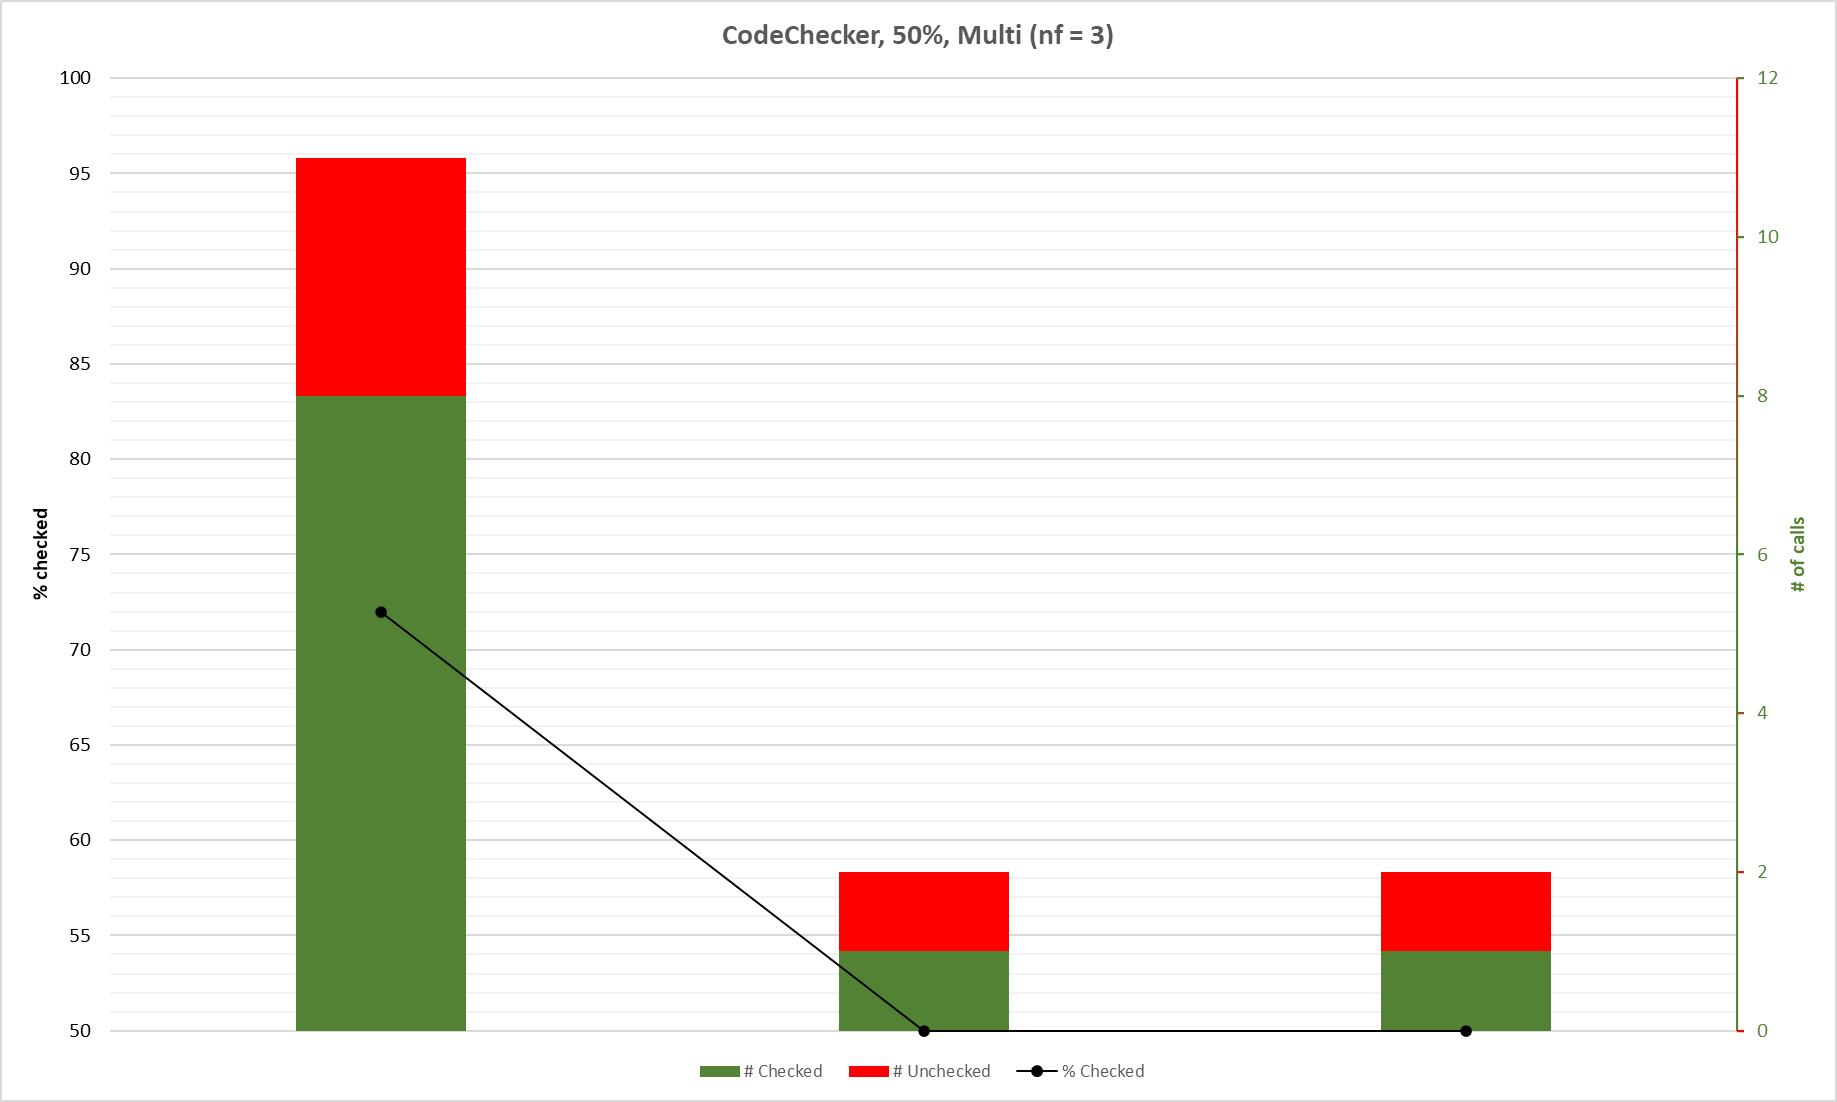
\includegraphics[width=1.2\linewidth]{images/appendix/CodeChecker_50_2_Multi.png}}
\end{figure}

\begin{figure}[H]
	\makebox[\textwidth]{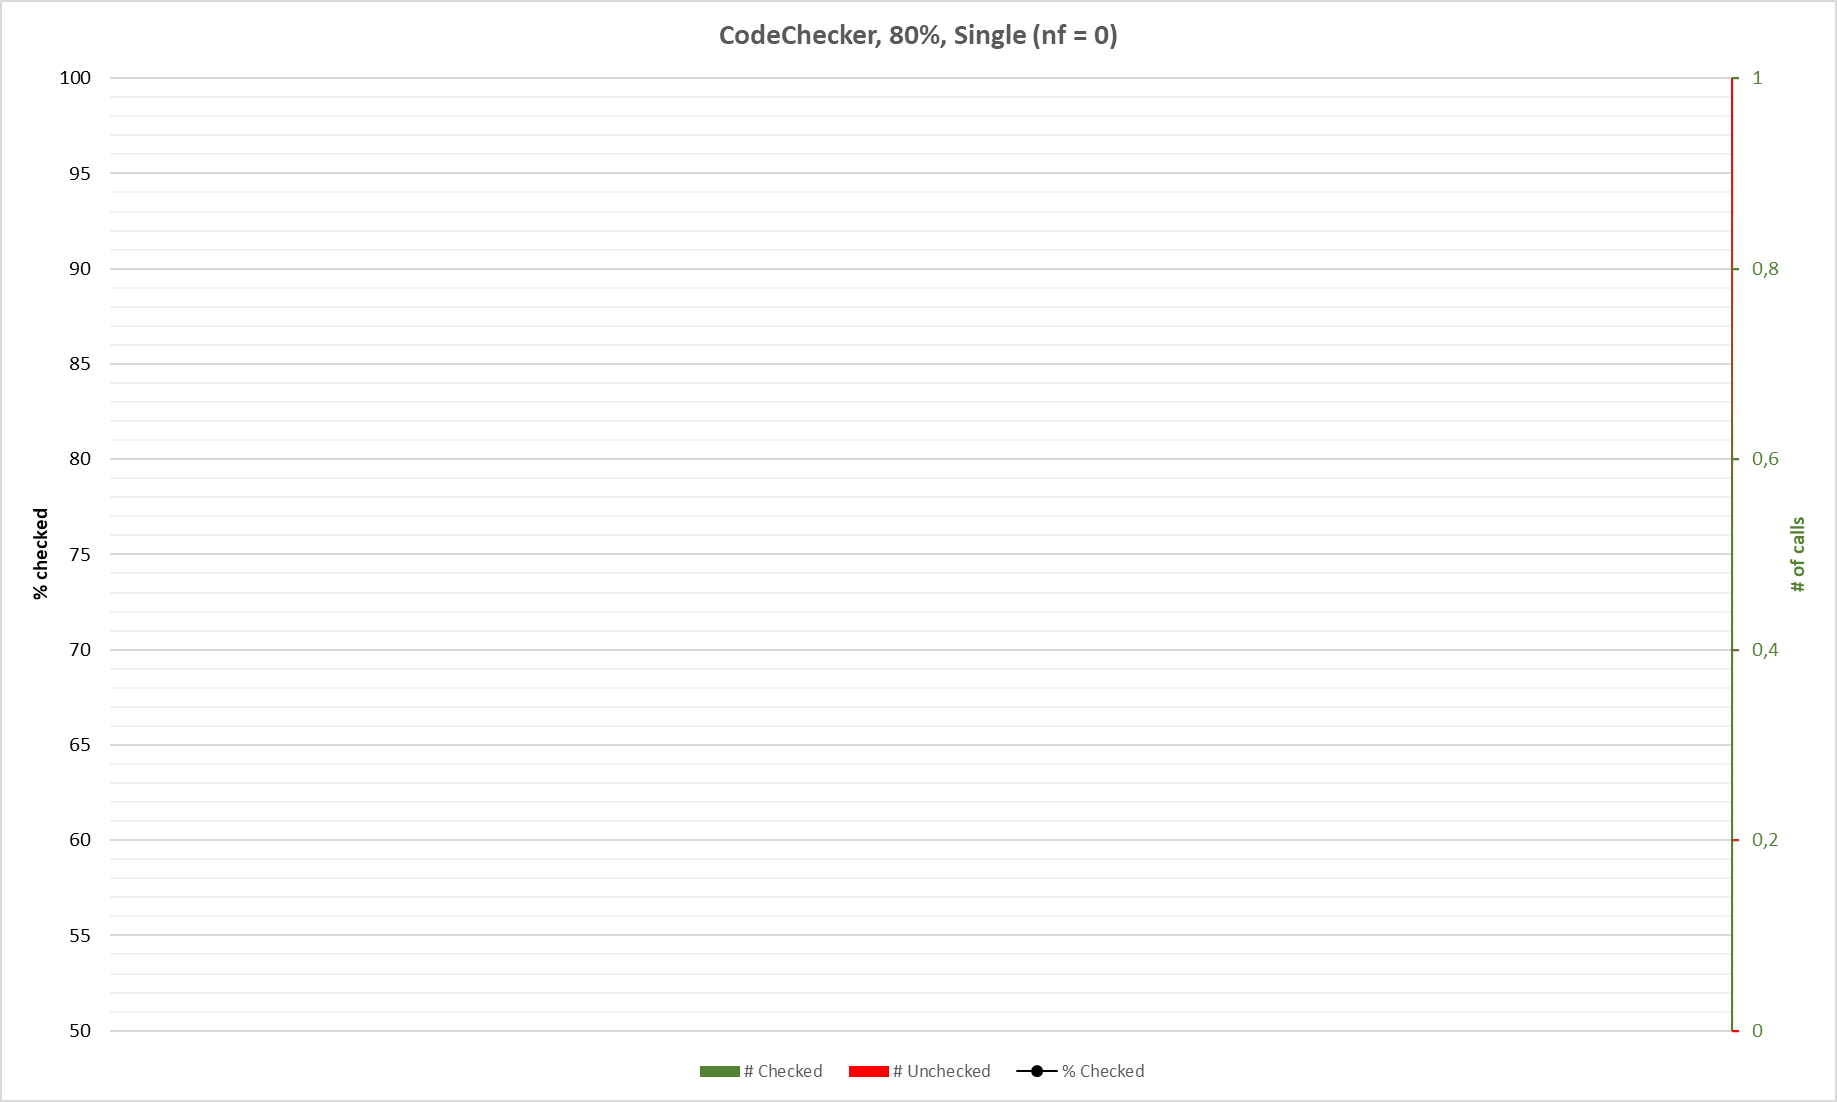
\includegraphics[width=1.2\linewidth]{images/appendix/CodeChecker_80_1_Single.png}}
\end{figure}

\begin{figure}[H]
	\makebox[\textwidth]{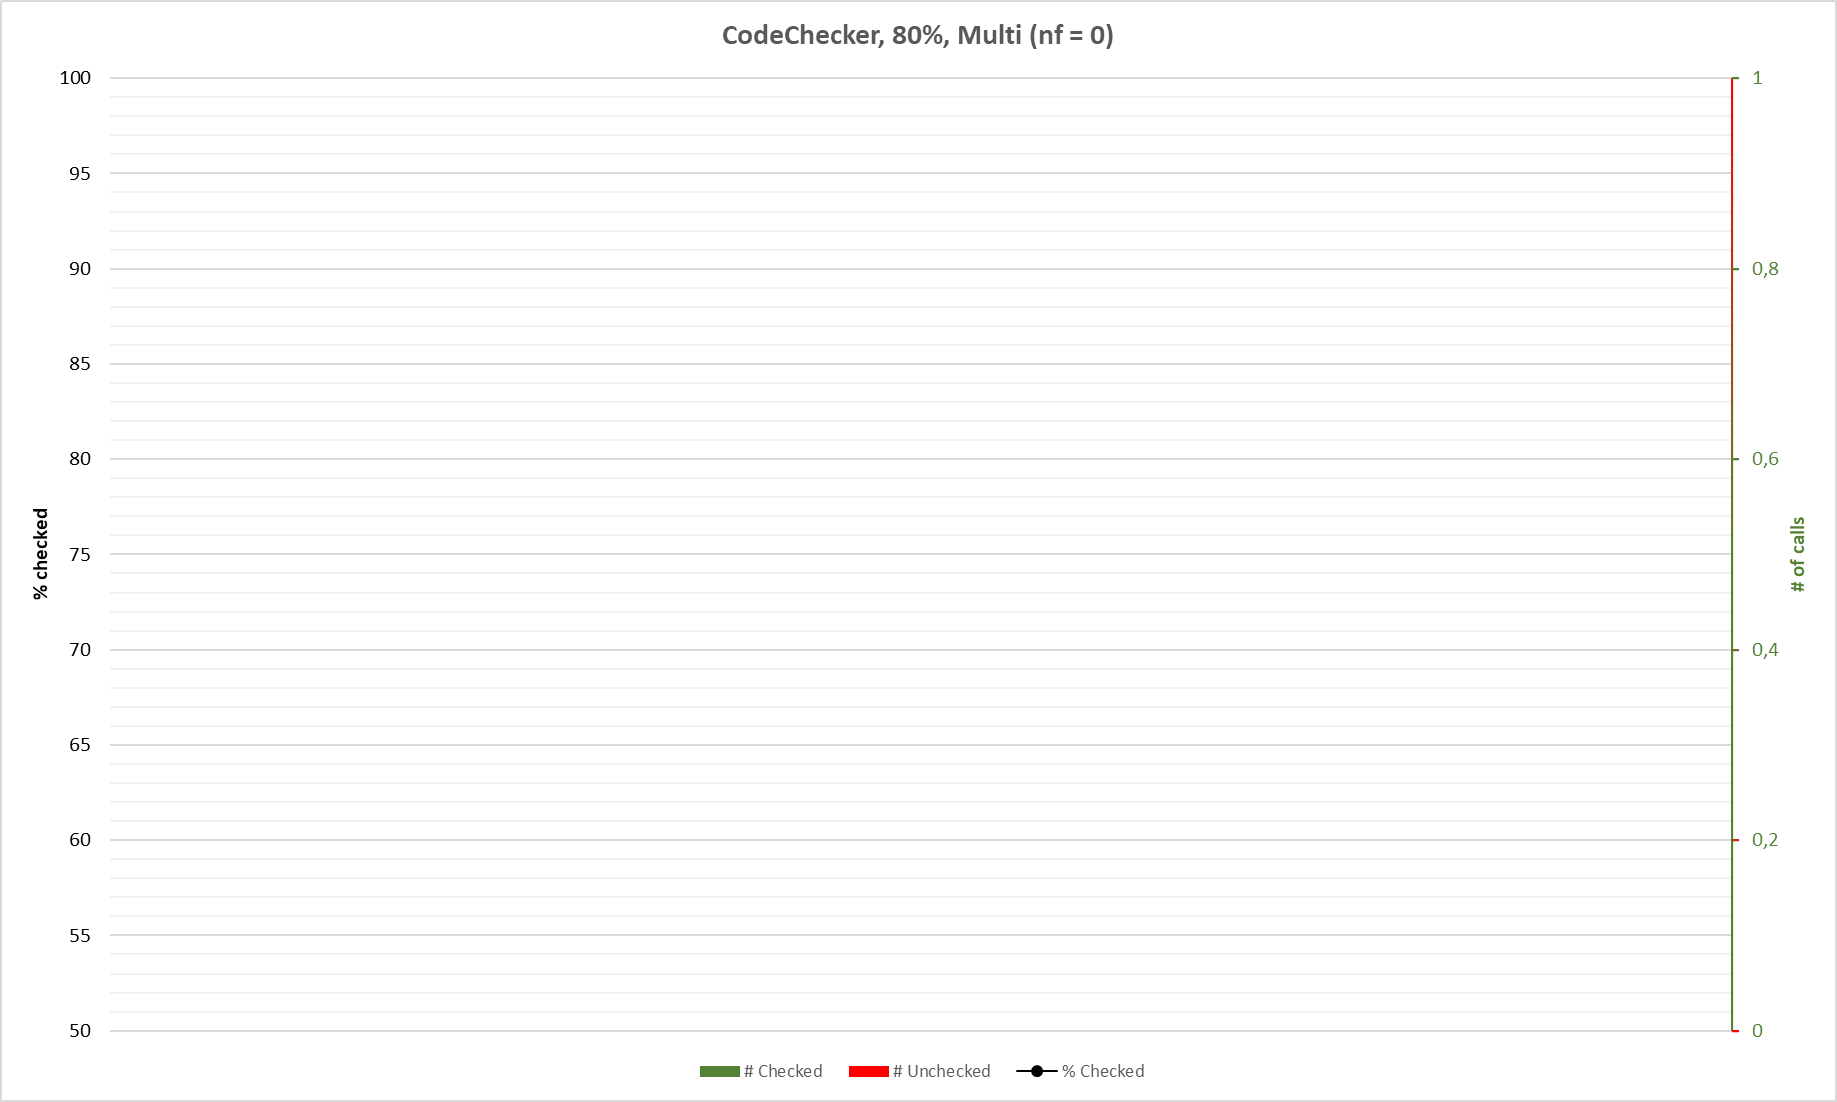
\includegraphics[width=1.2\linewidth]{images/appendix/CodeChecker_80_2_Multi.png}}
\end{figure}

\begin{figure}[H]
	\makebox[\textwidth]{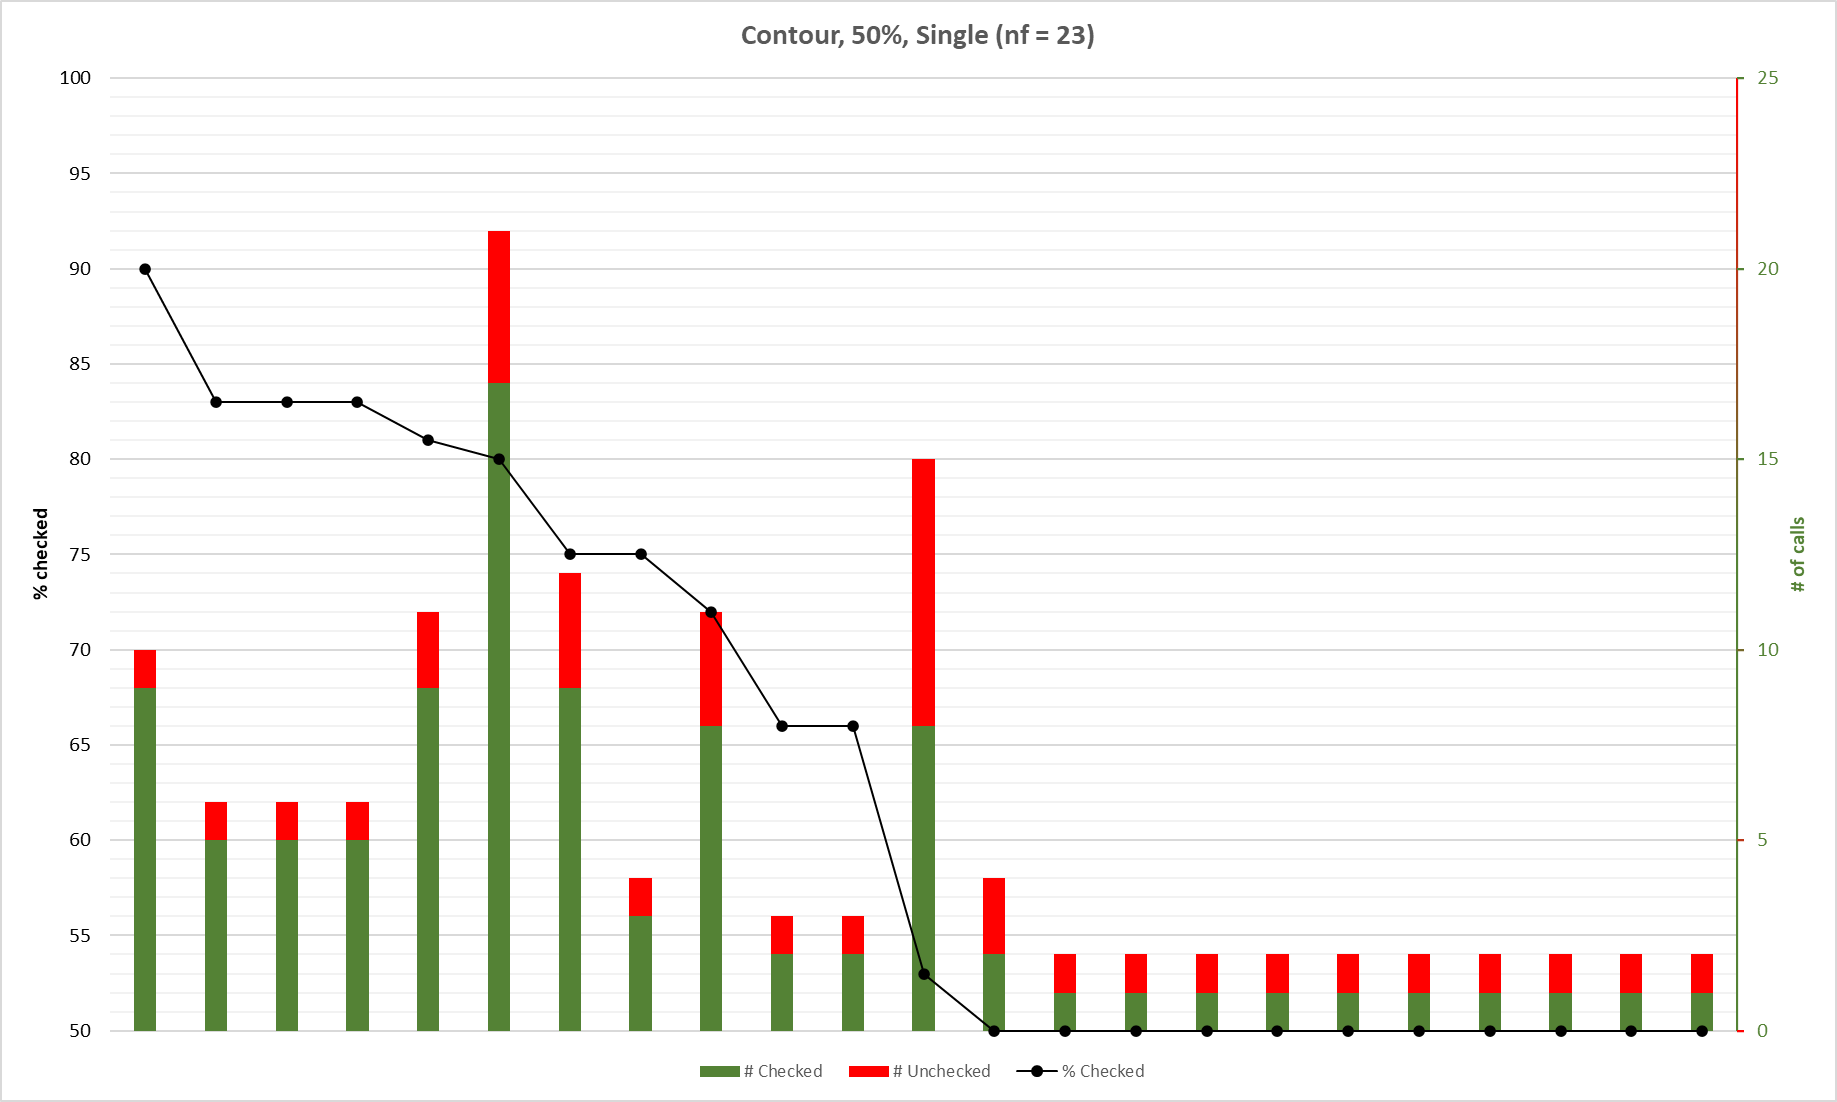
\includegraphics[width=1.2\linewidth]{images/appendix/Contour_50_1_Single.png}}
\end{figure}

\begin{figure}[H]
	\makebox[\textwidth]{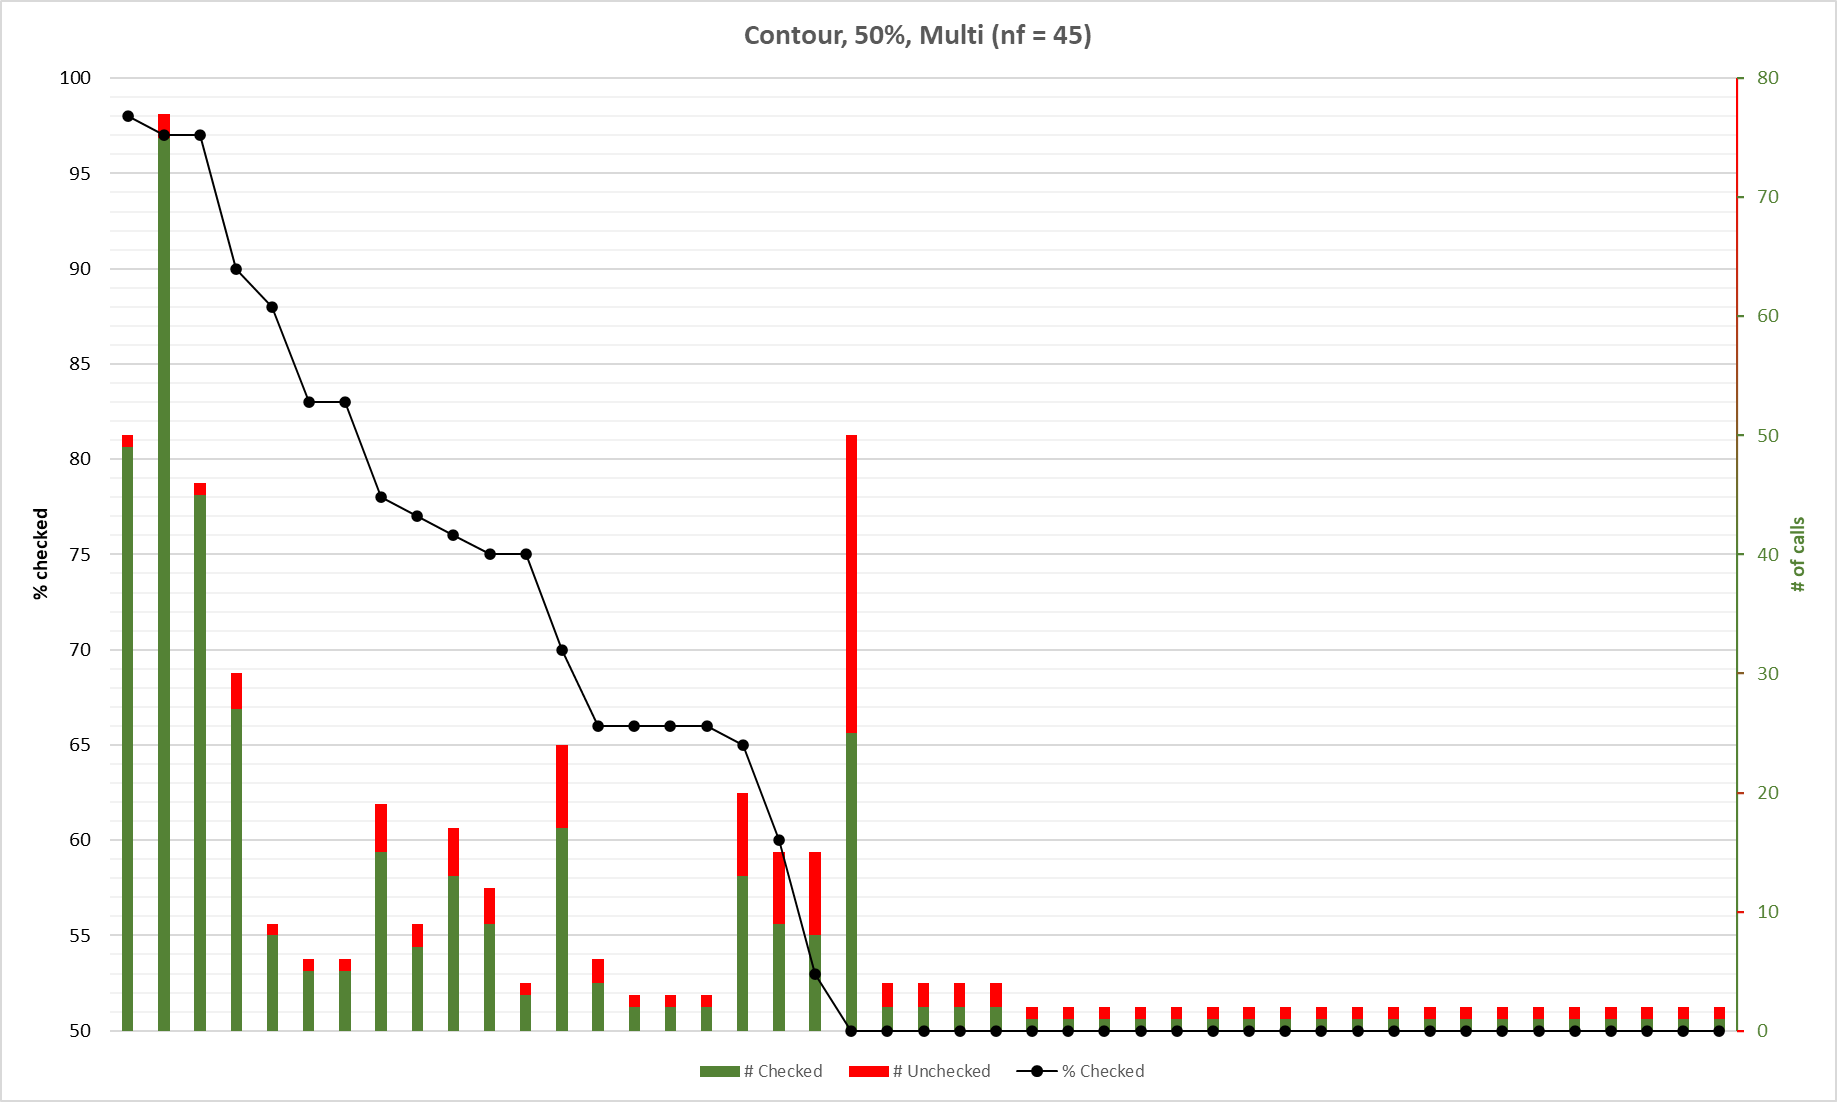
\includegraphics[width=1.2\linewidth]{images/appendix/Contour_50_2_Multi.png}}
\end{figure}

\begin{figure}[H]
	\makebox[\textwidth]{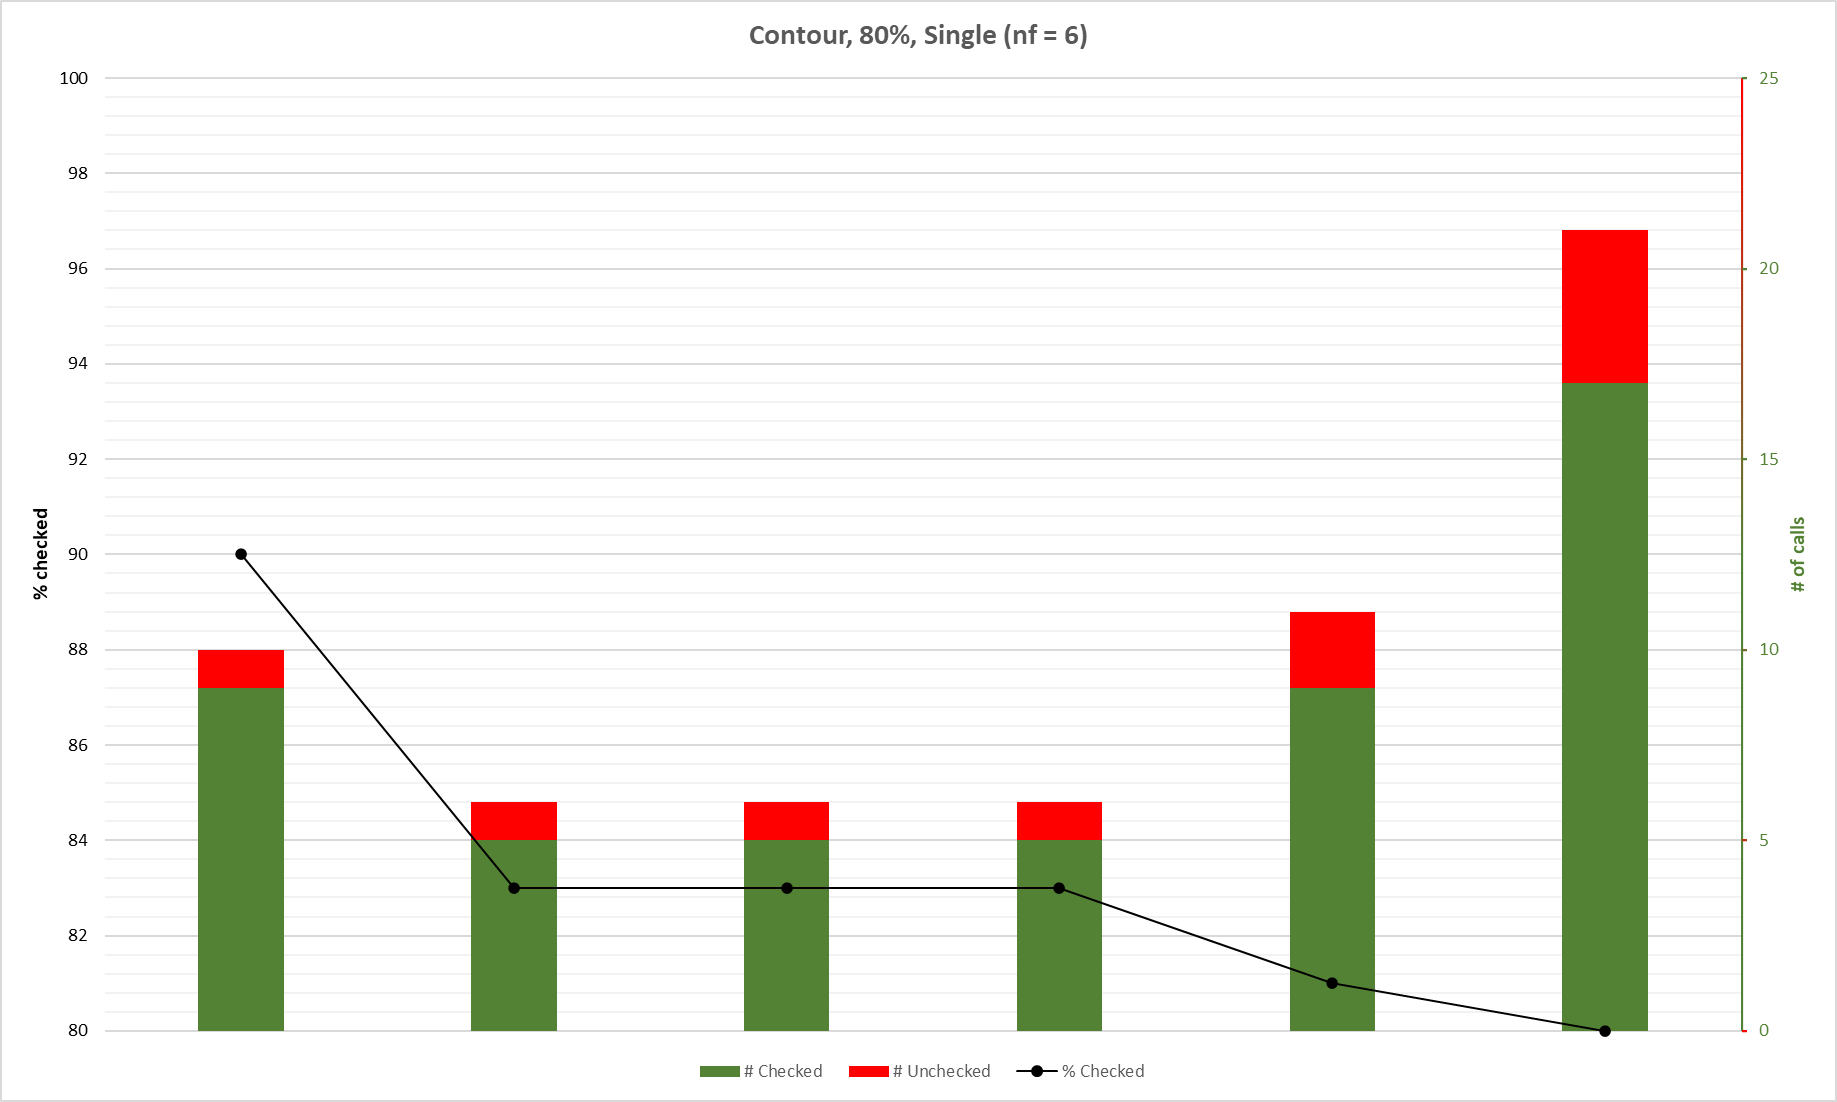
\includegraphics[width=1.2\linewidth]{images/appendix/Contour_80_1_Single.png}}
\end{figure}

\begin{figure}[H]
	\makebox[\textwidth]{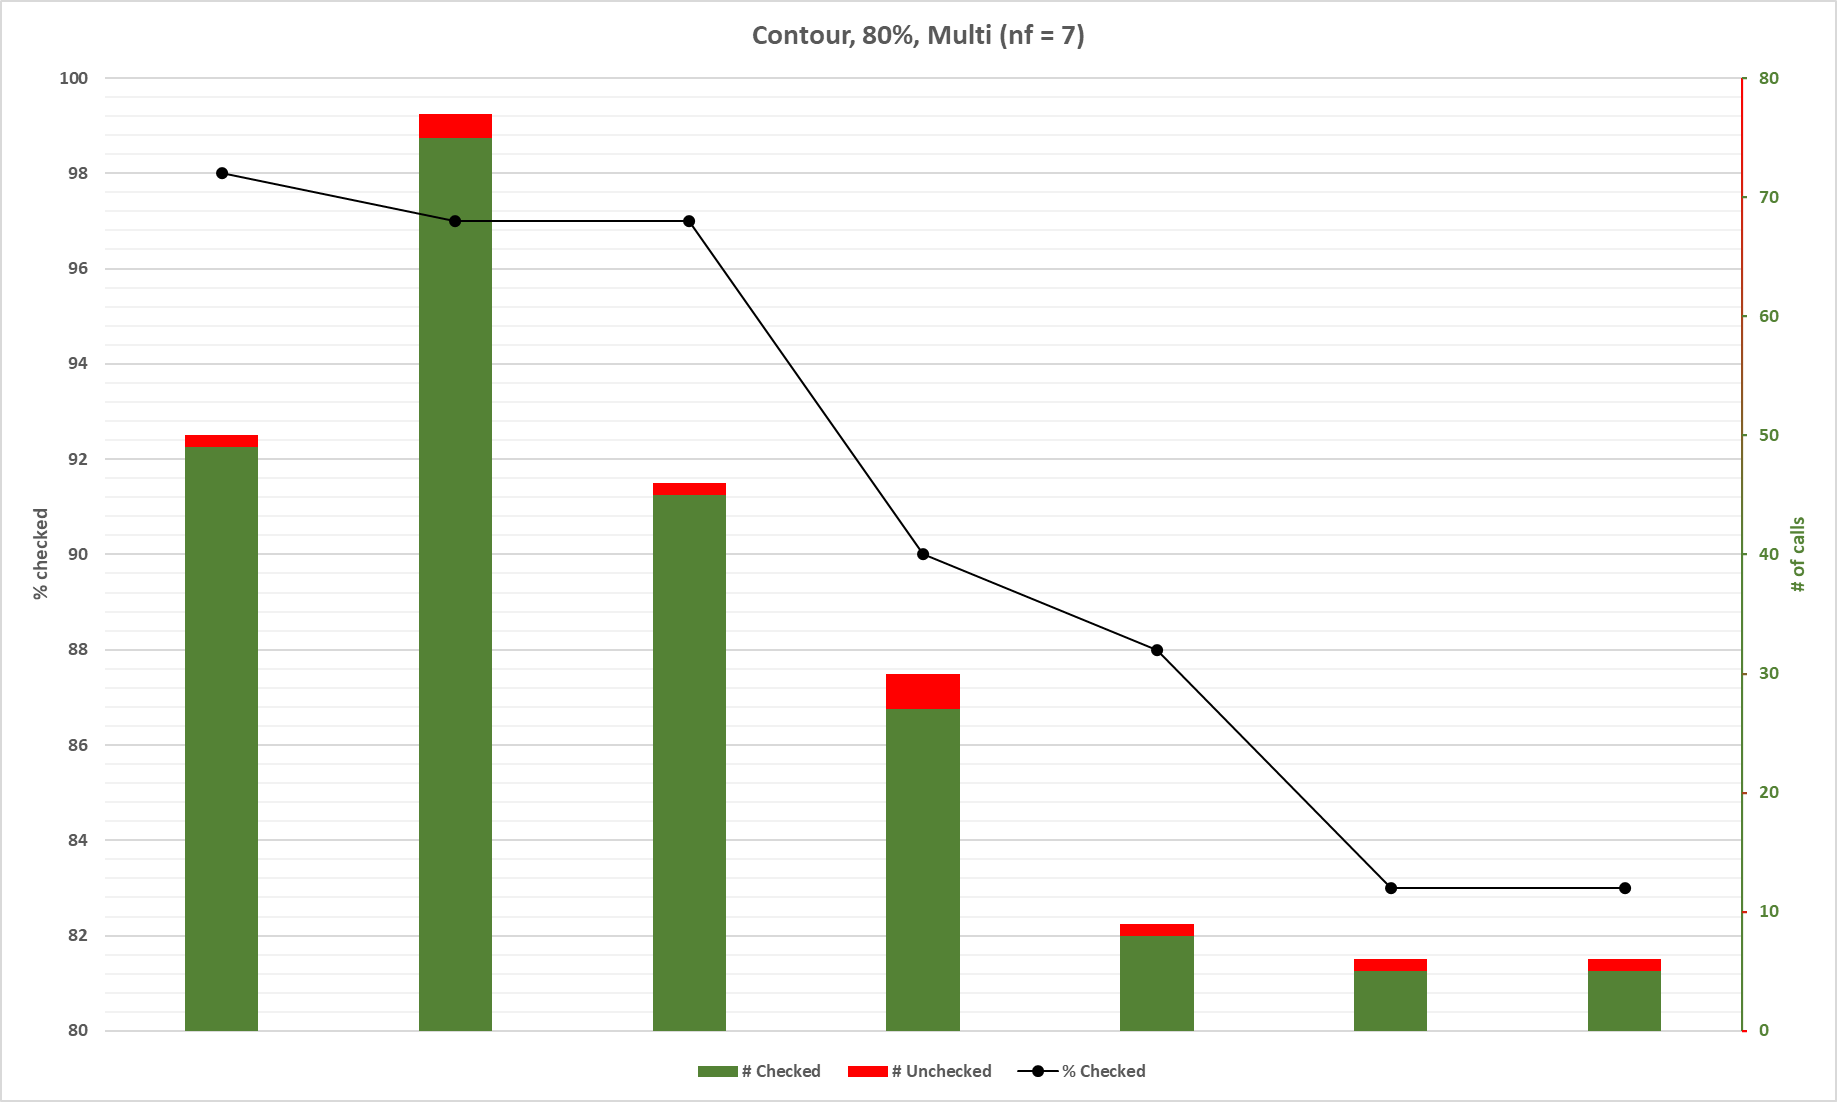
\includegraphics[width=1.2\linewidth]{images/appendix/Contour_80_2_Multi.png}}
\end{figure}

\begin{figure}[H]
	\makebox[\textwidth]{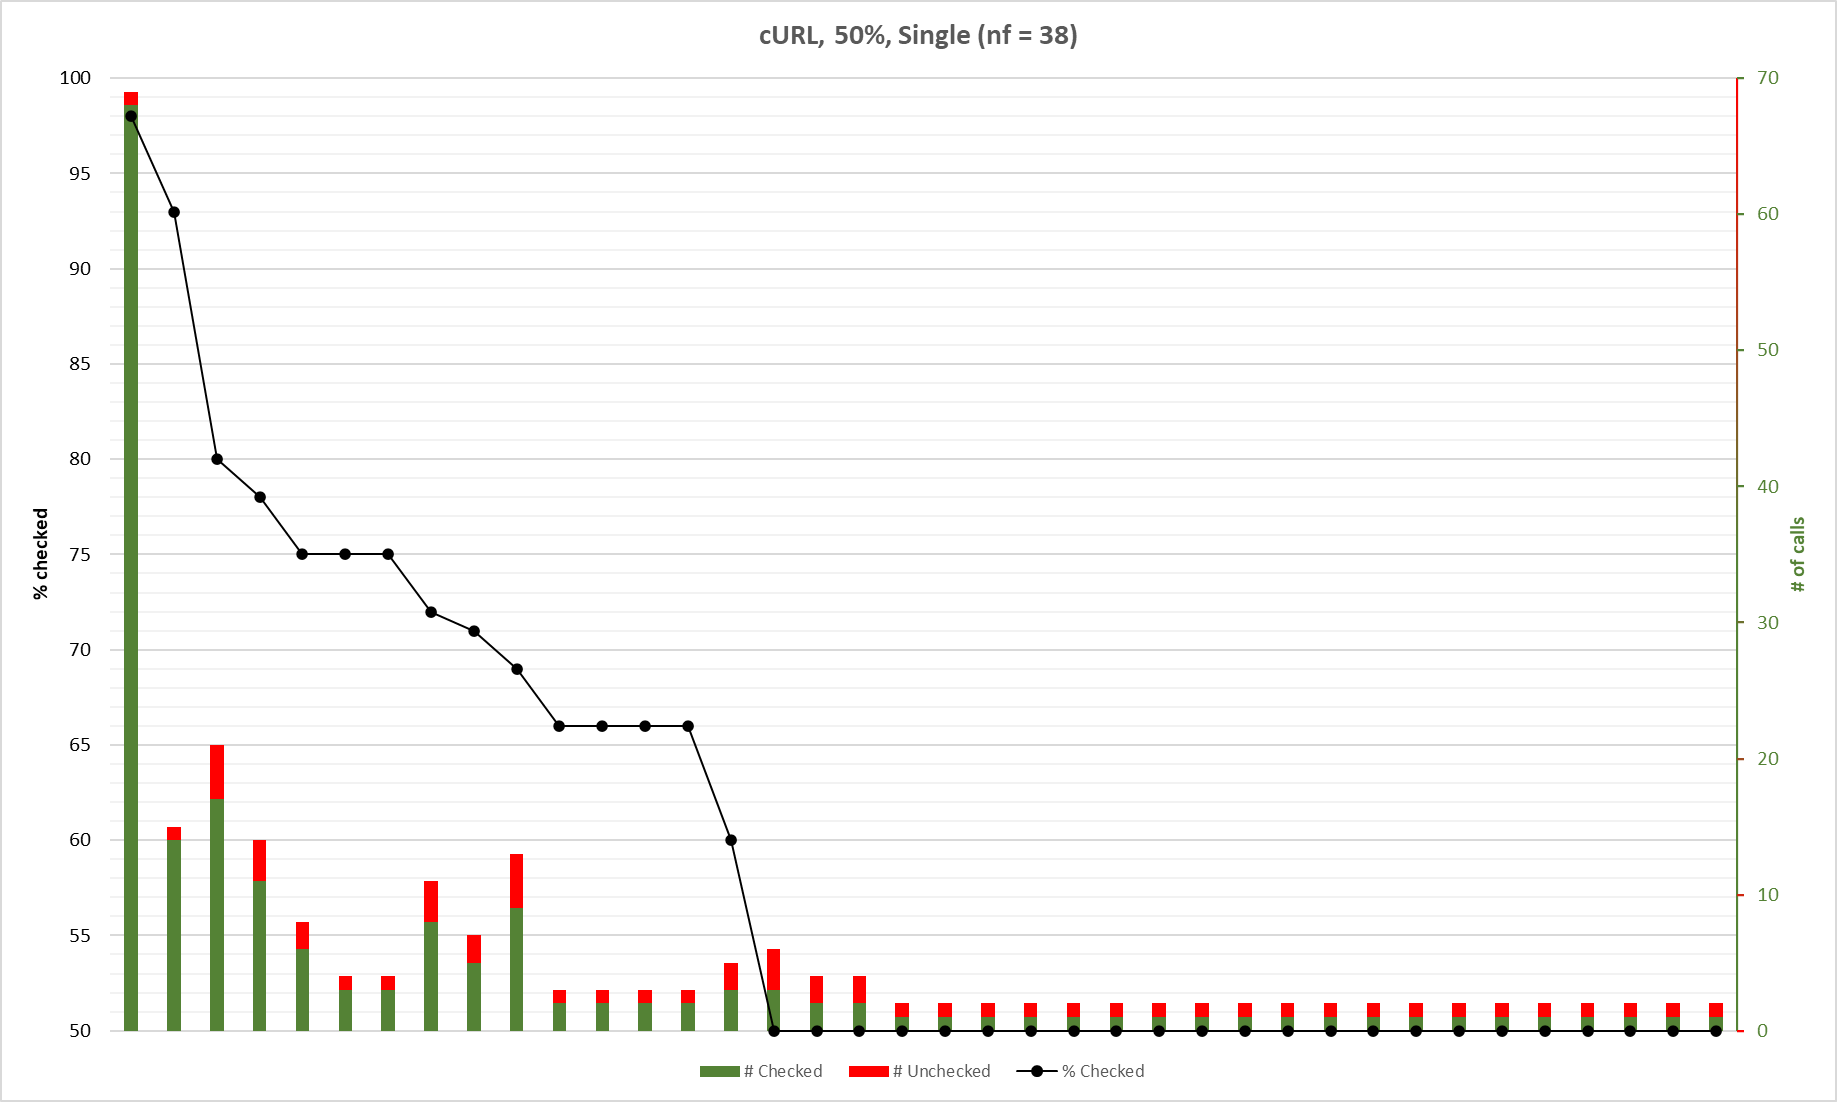
\includegraphics[width=1.2\linewidth]{images/appendix/cURL_50_1_Single.png}}
\end{figure}

\begin{figure}[H]
	\makebox[\textwidth]{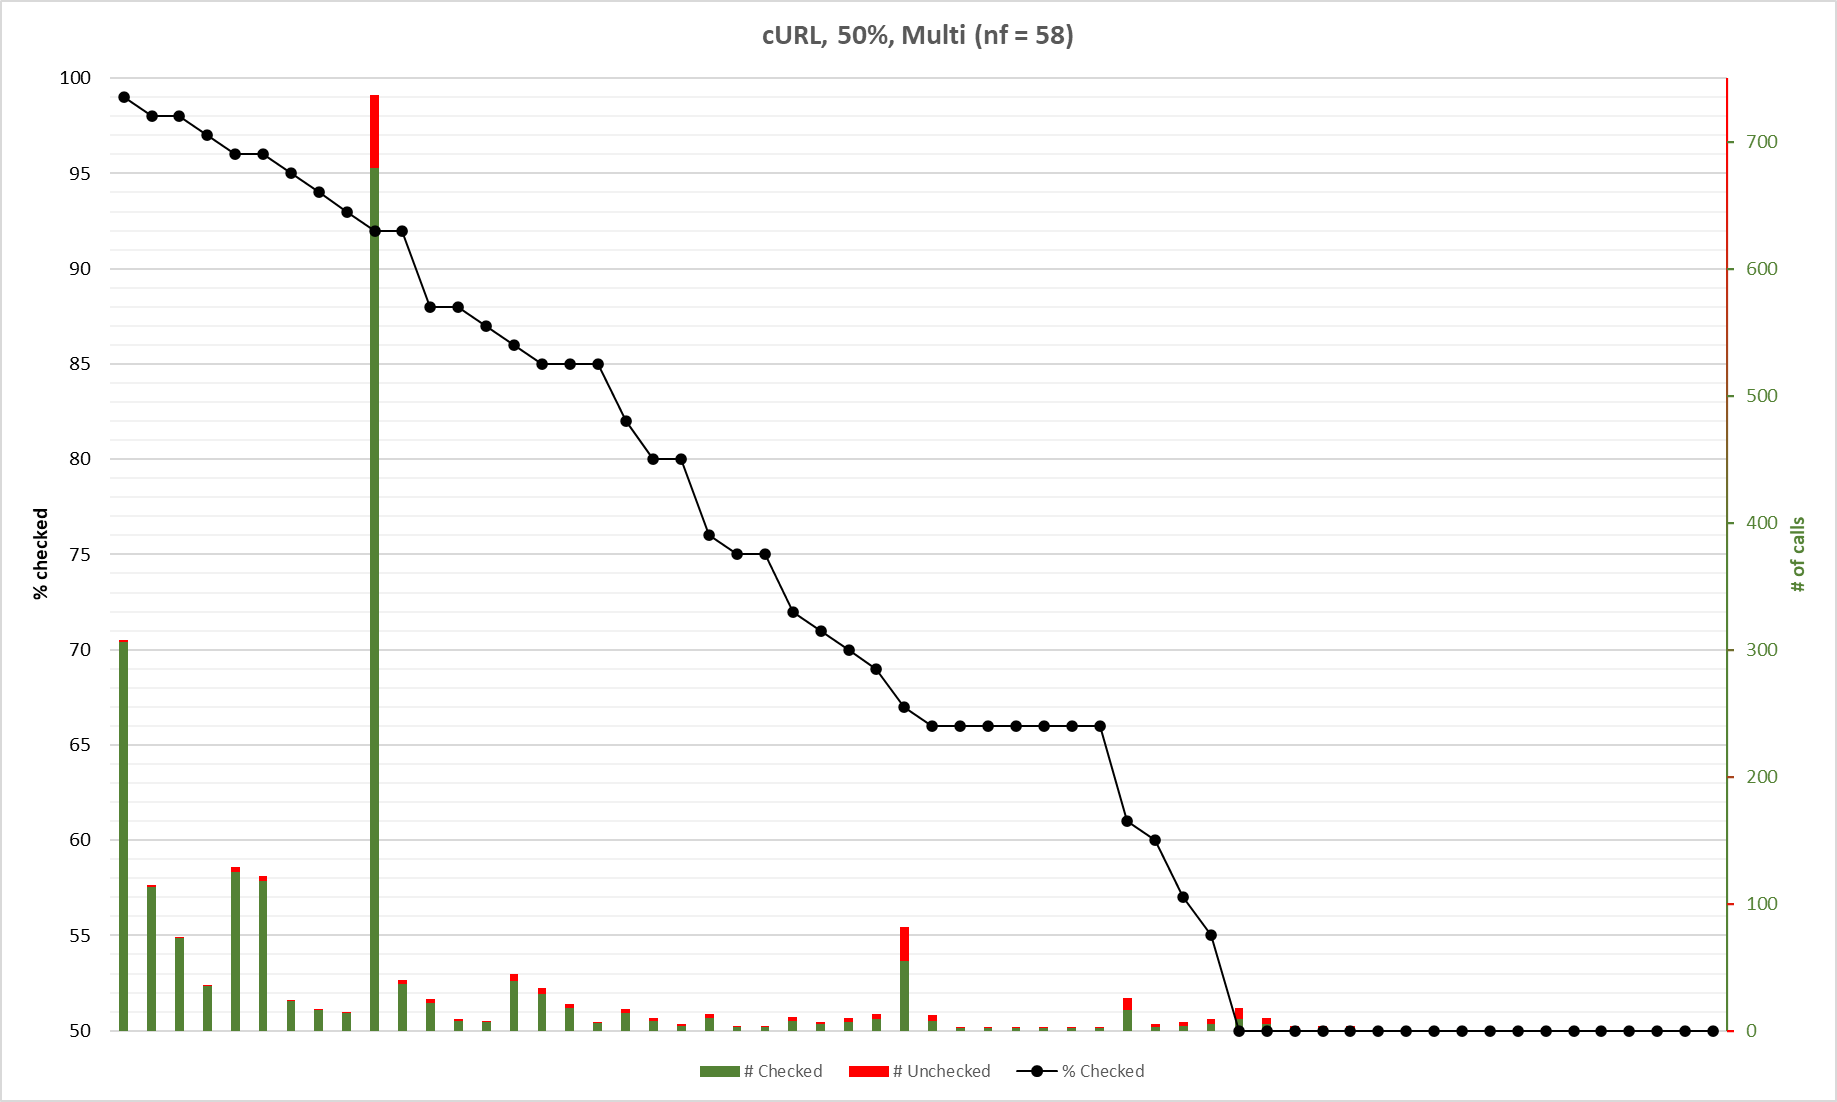
\includegraphics[width=1.2\linewidth]{images/appendix/cURL_50_2_Multi.png}}
\end{figure}

\begin{figure}[H]
	\makebox[\textwidth]{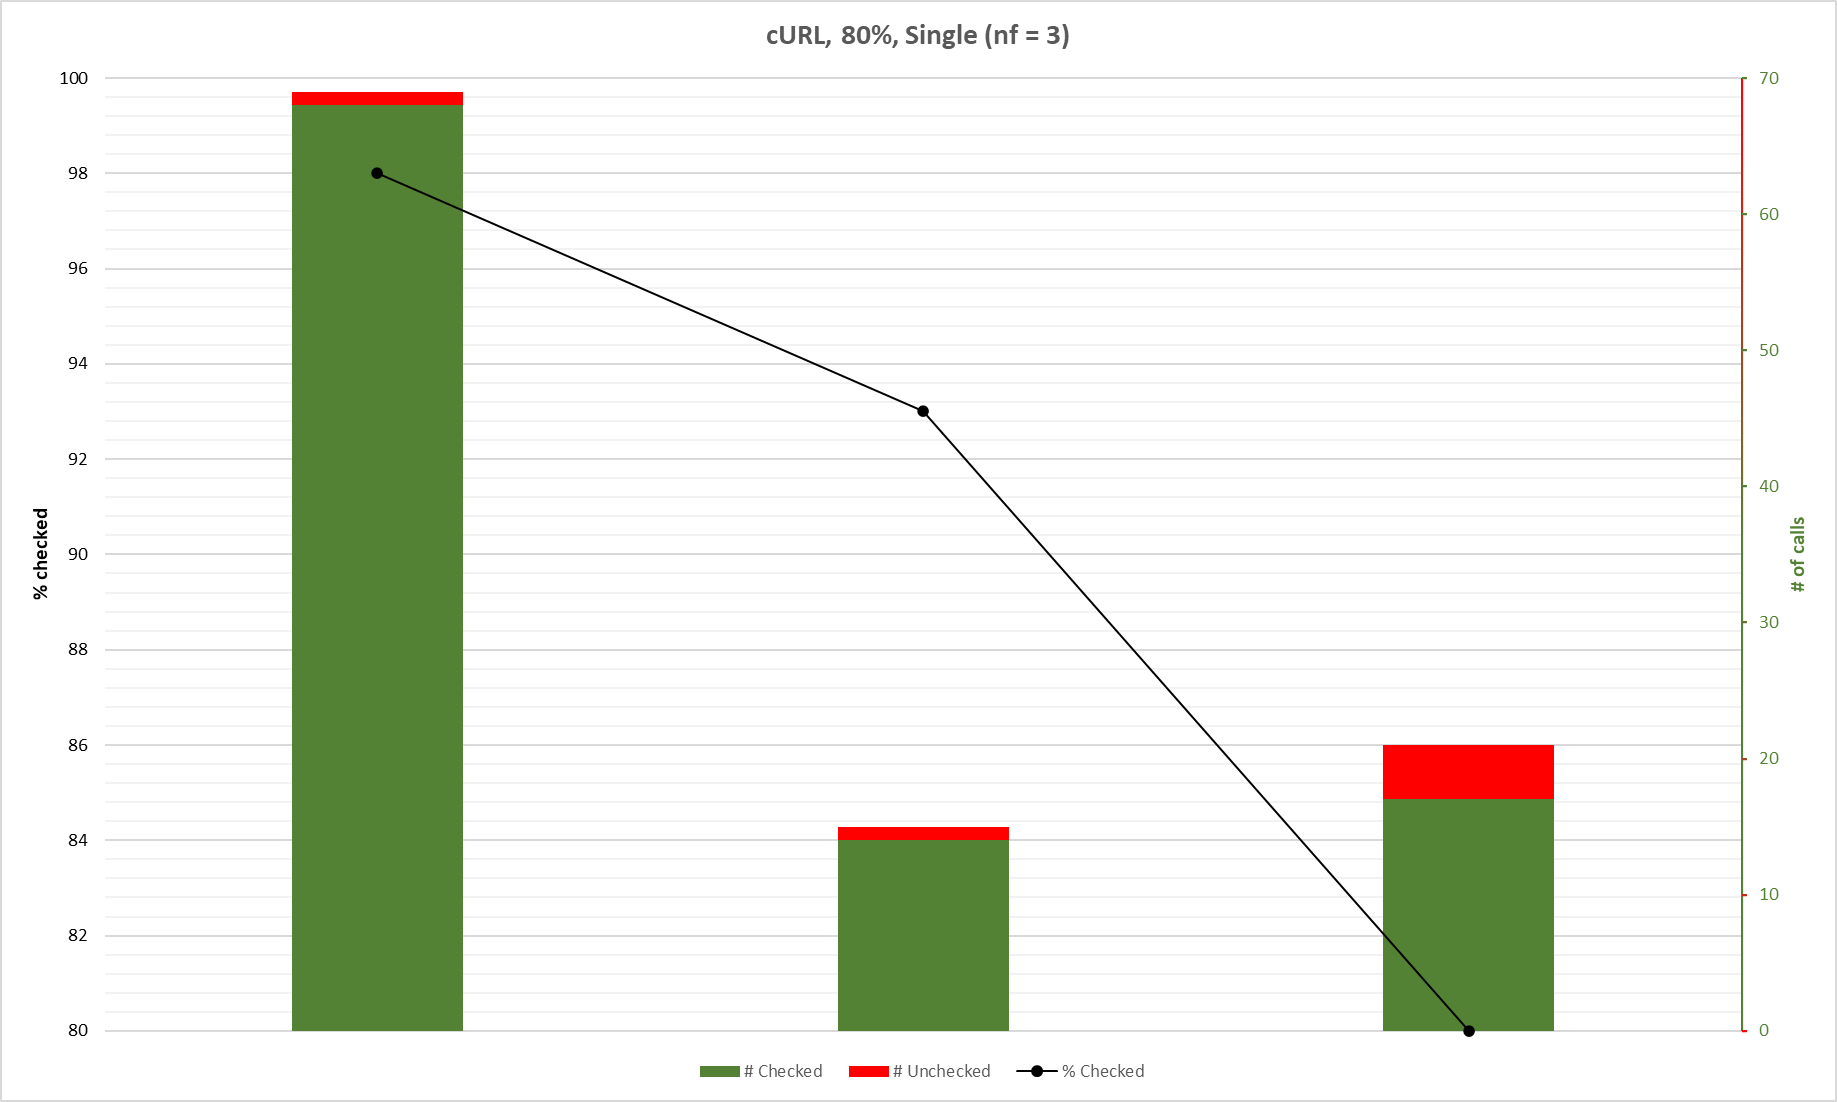
\includegraphics[width=1.2\linewidth]{images/appendix/cURL_80_1_Single.png}}
\end{figure}

\begin{figure}[H]
	\makebox[\textwidth]{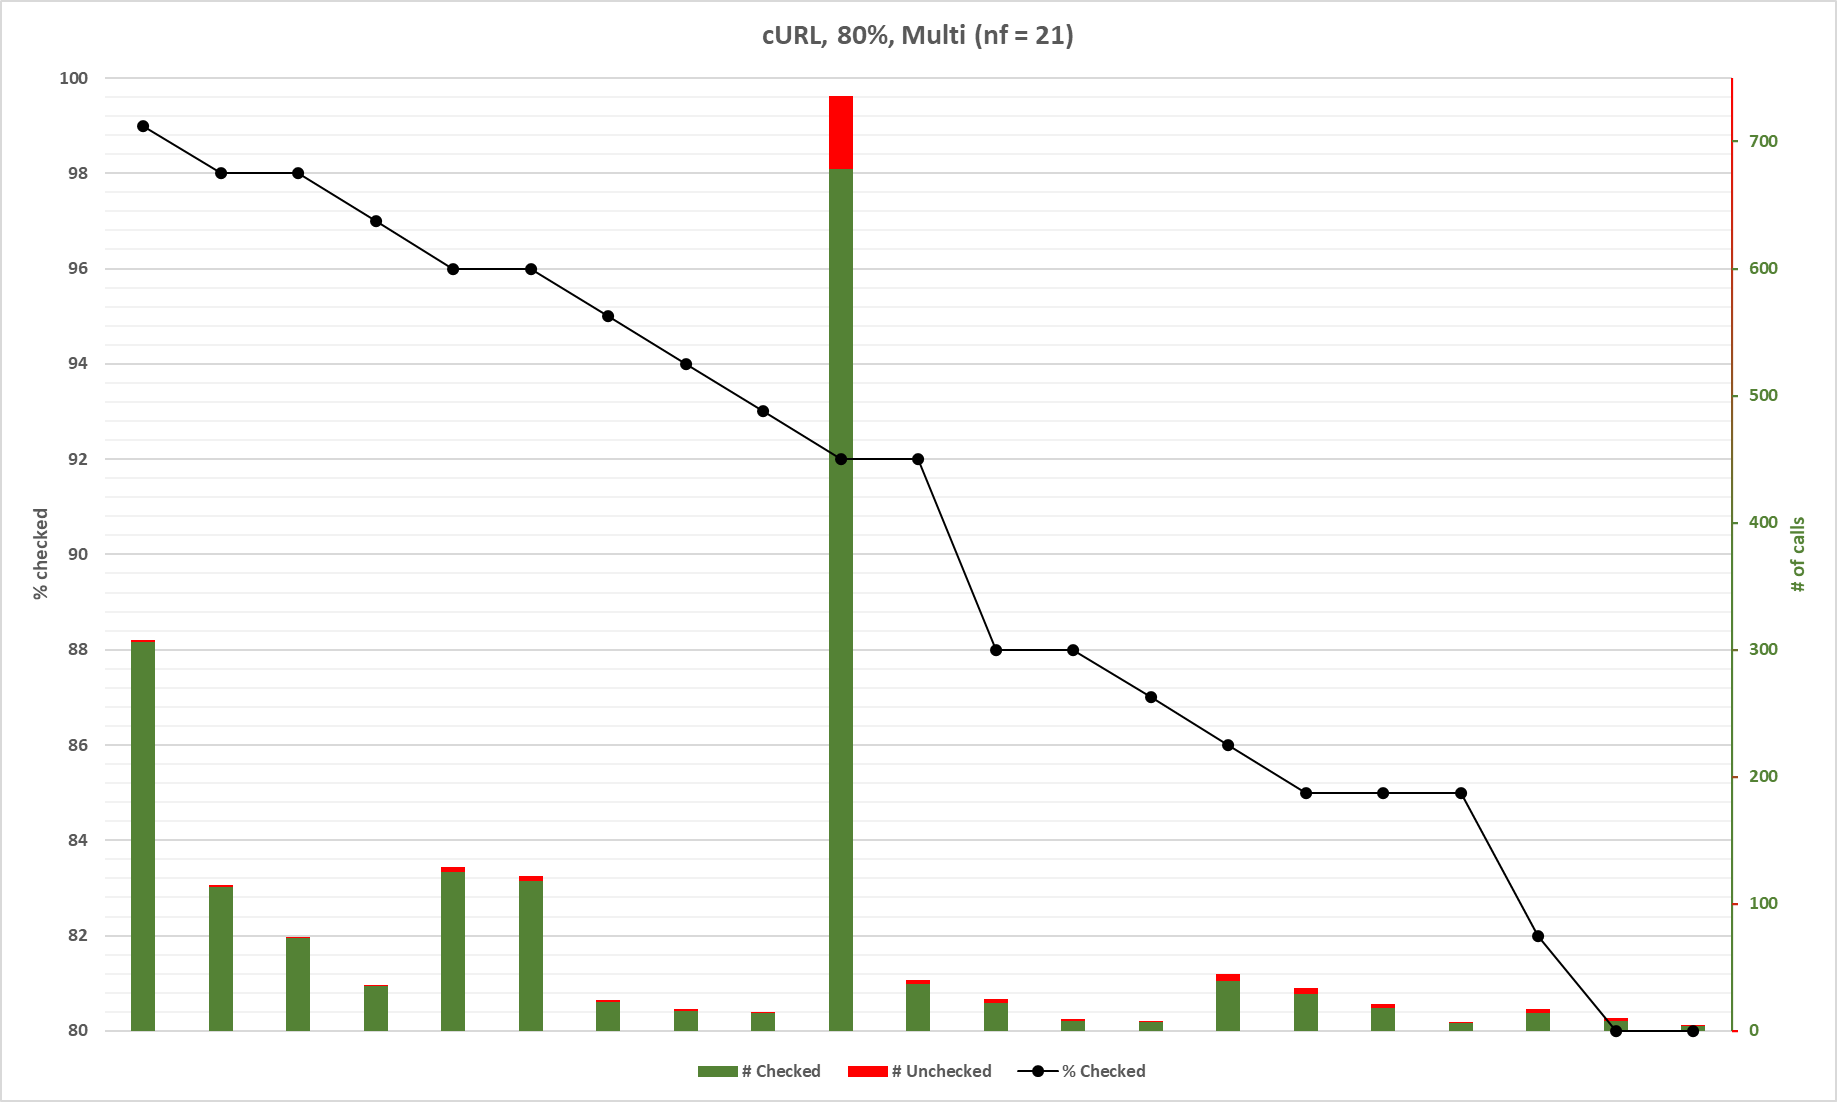
\includegraphics[width=1.2\linewidth]{images/appendix/cURL_80_2_Multi.png}}
\end{figure}

\begin{figure}[H]
	\makebox[\textwidth]{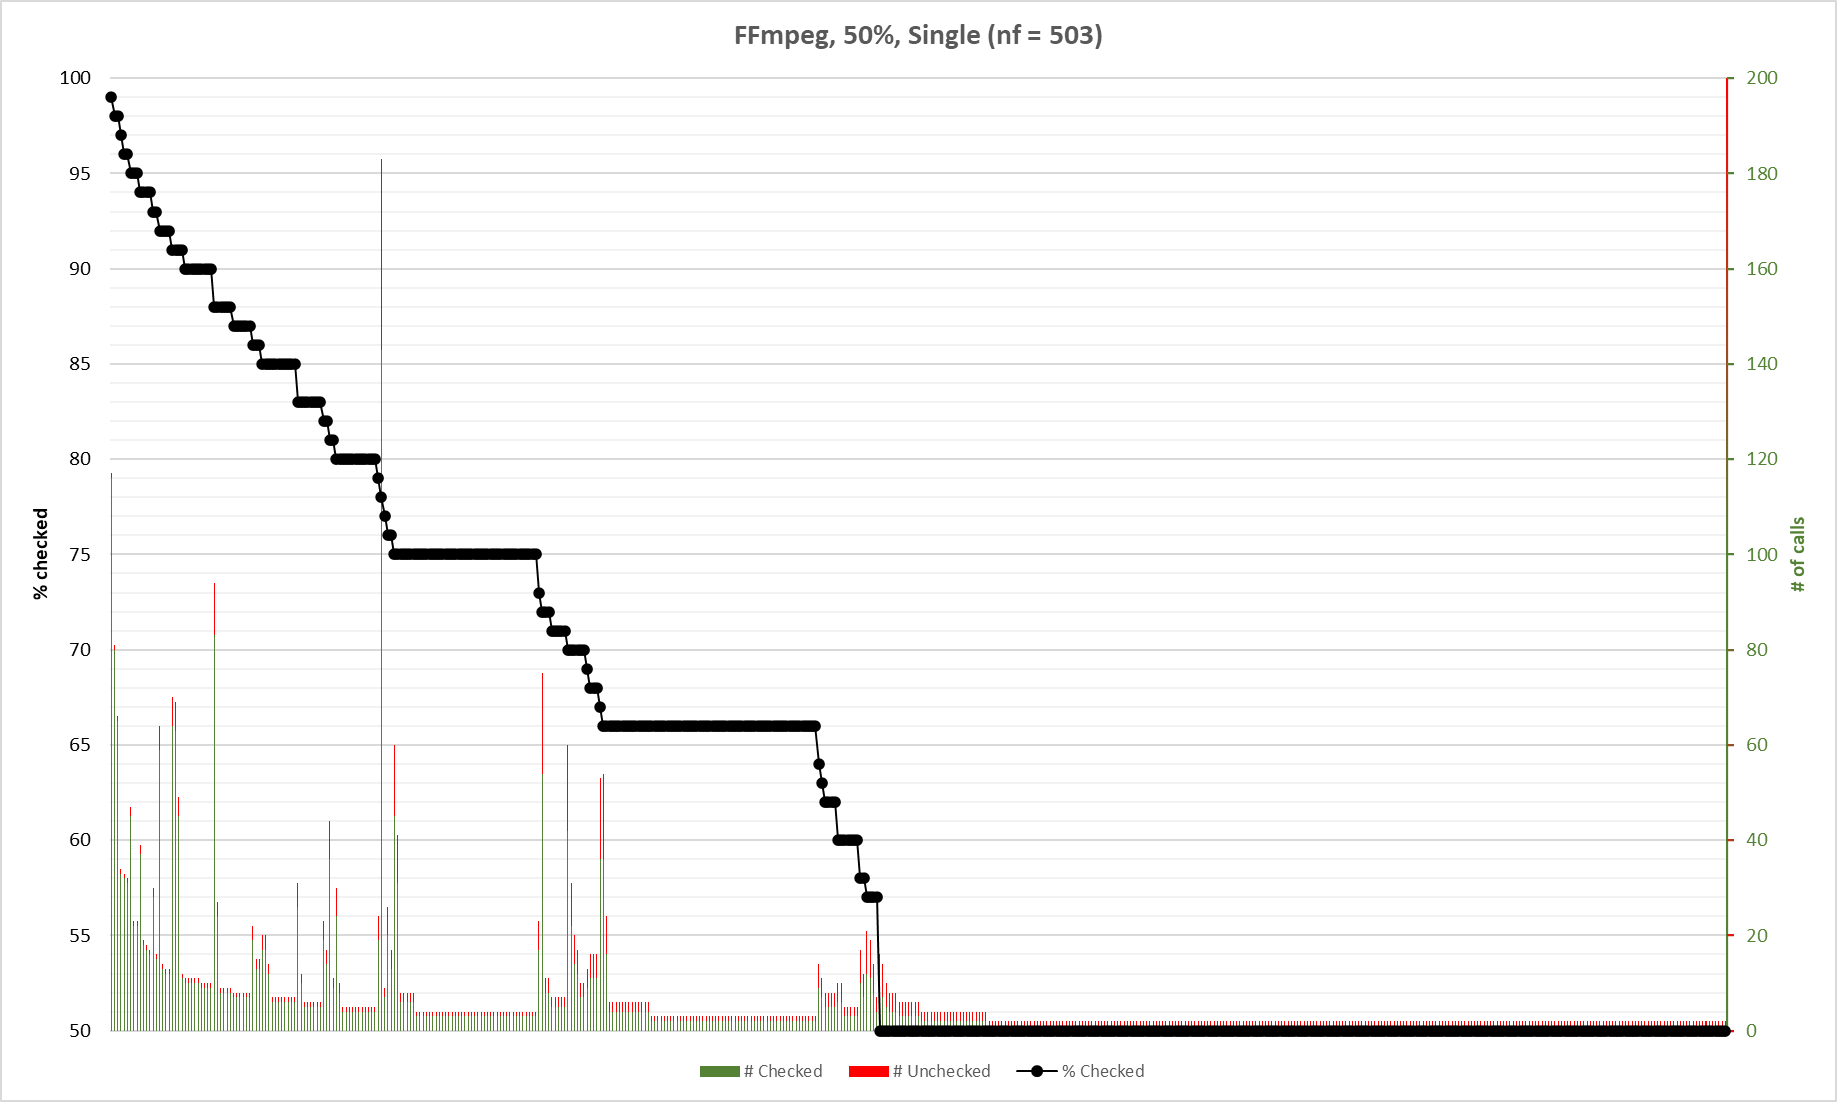
\includegraphics[width=1.2\linewidth]{images/appendix/FFmpeg_50_1_Single.png}}
\end{figure}

\begin{figure}[H]
	\makebox[\textwidth]{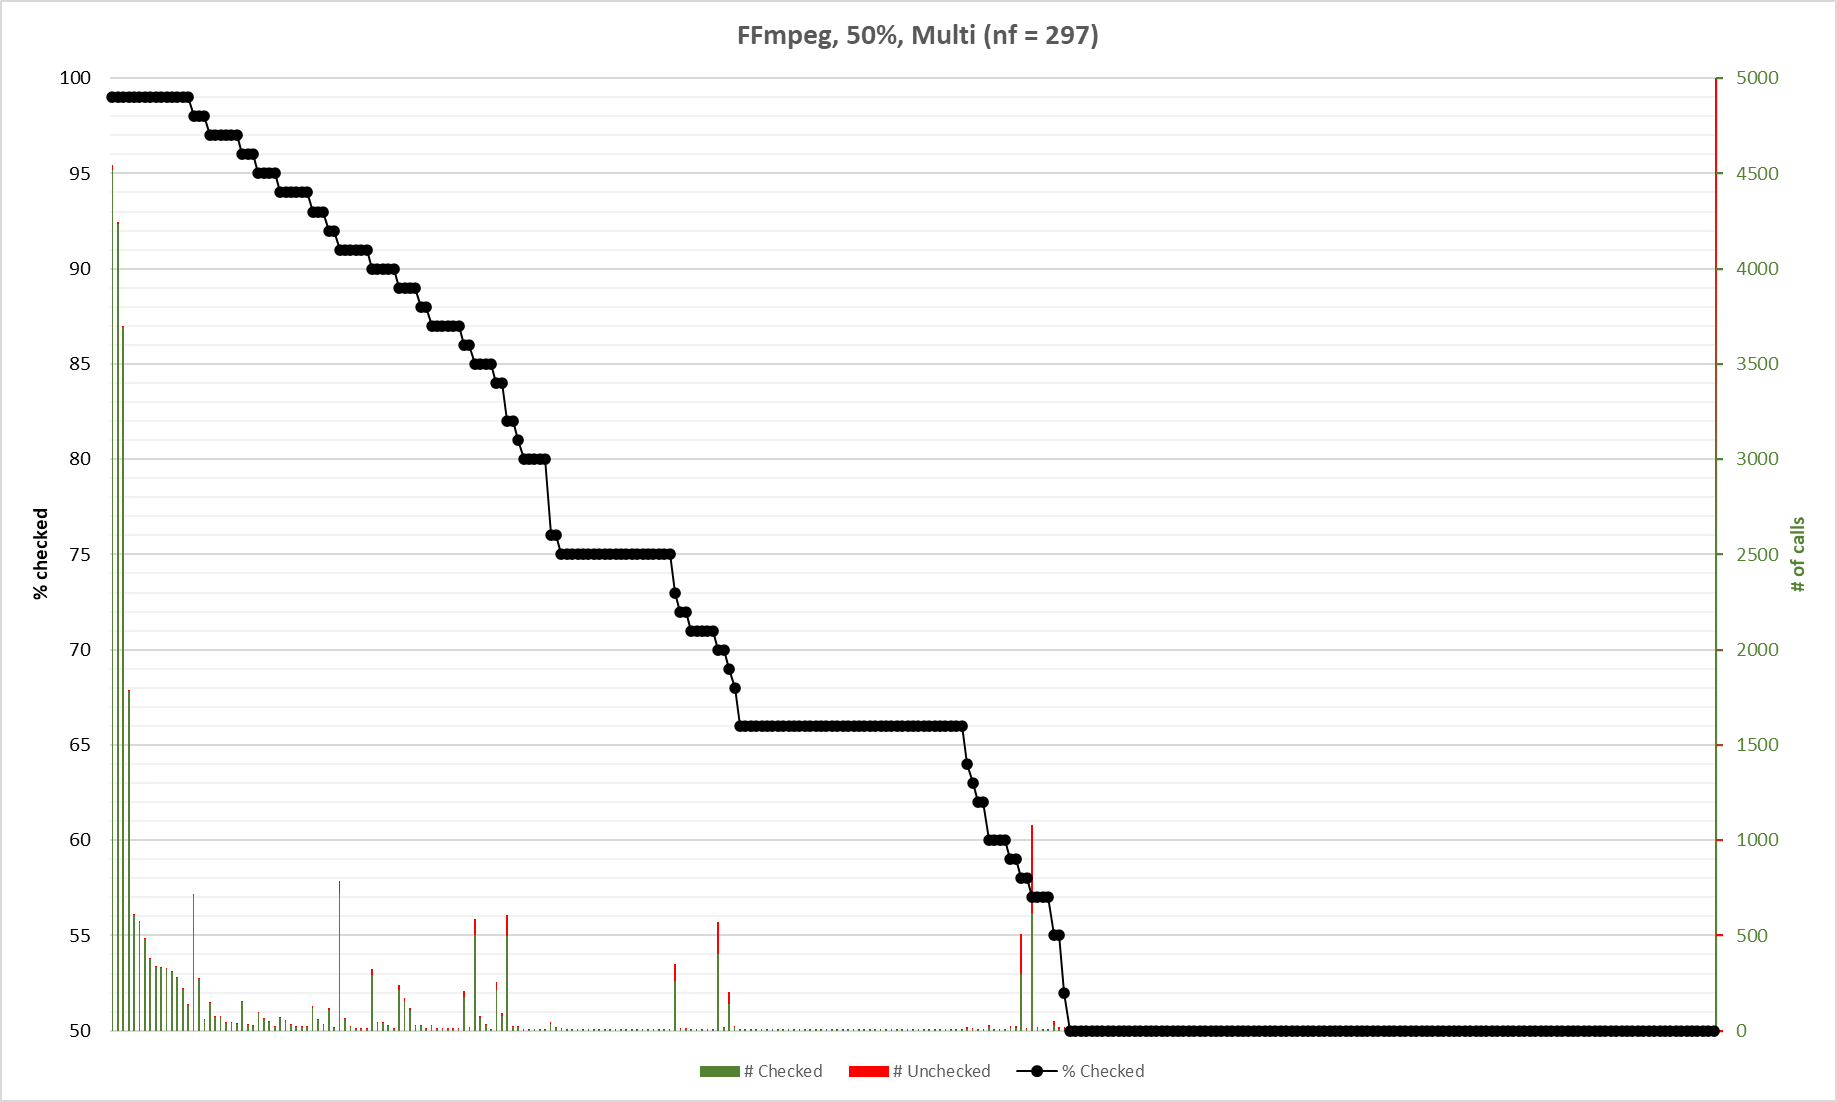
\includegraphics[width=1.2\linewidth]{images/appendix/FFmpeg_50_2_Multi.png}}
\end{figure}

\begin{figure}[H]
	\makebox[\textwidth]{\includegraphics[width=1.2\linewidth]{images/appendix/FFmpeg_80_1_Single.png}}
\end{figure}

\begin{figure}[H]
	\makebox[\textwidth]{\includegraphics[width=1.2\linewidth]{images/appendix/FFmpeg_80_2_Multi.png}}
\end{figure}

\begin{figure}[H]
	\makebox[\textwidth]{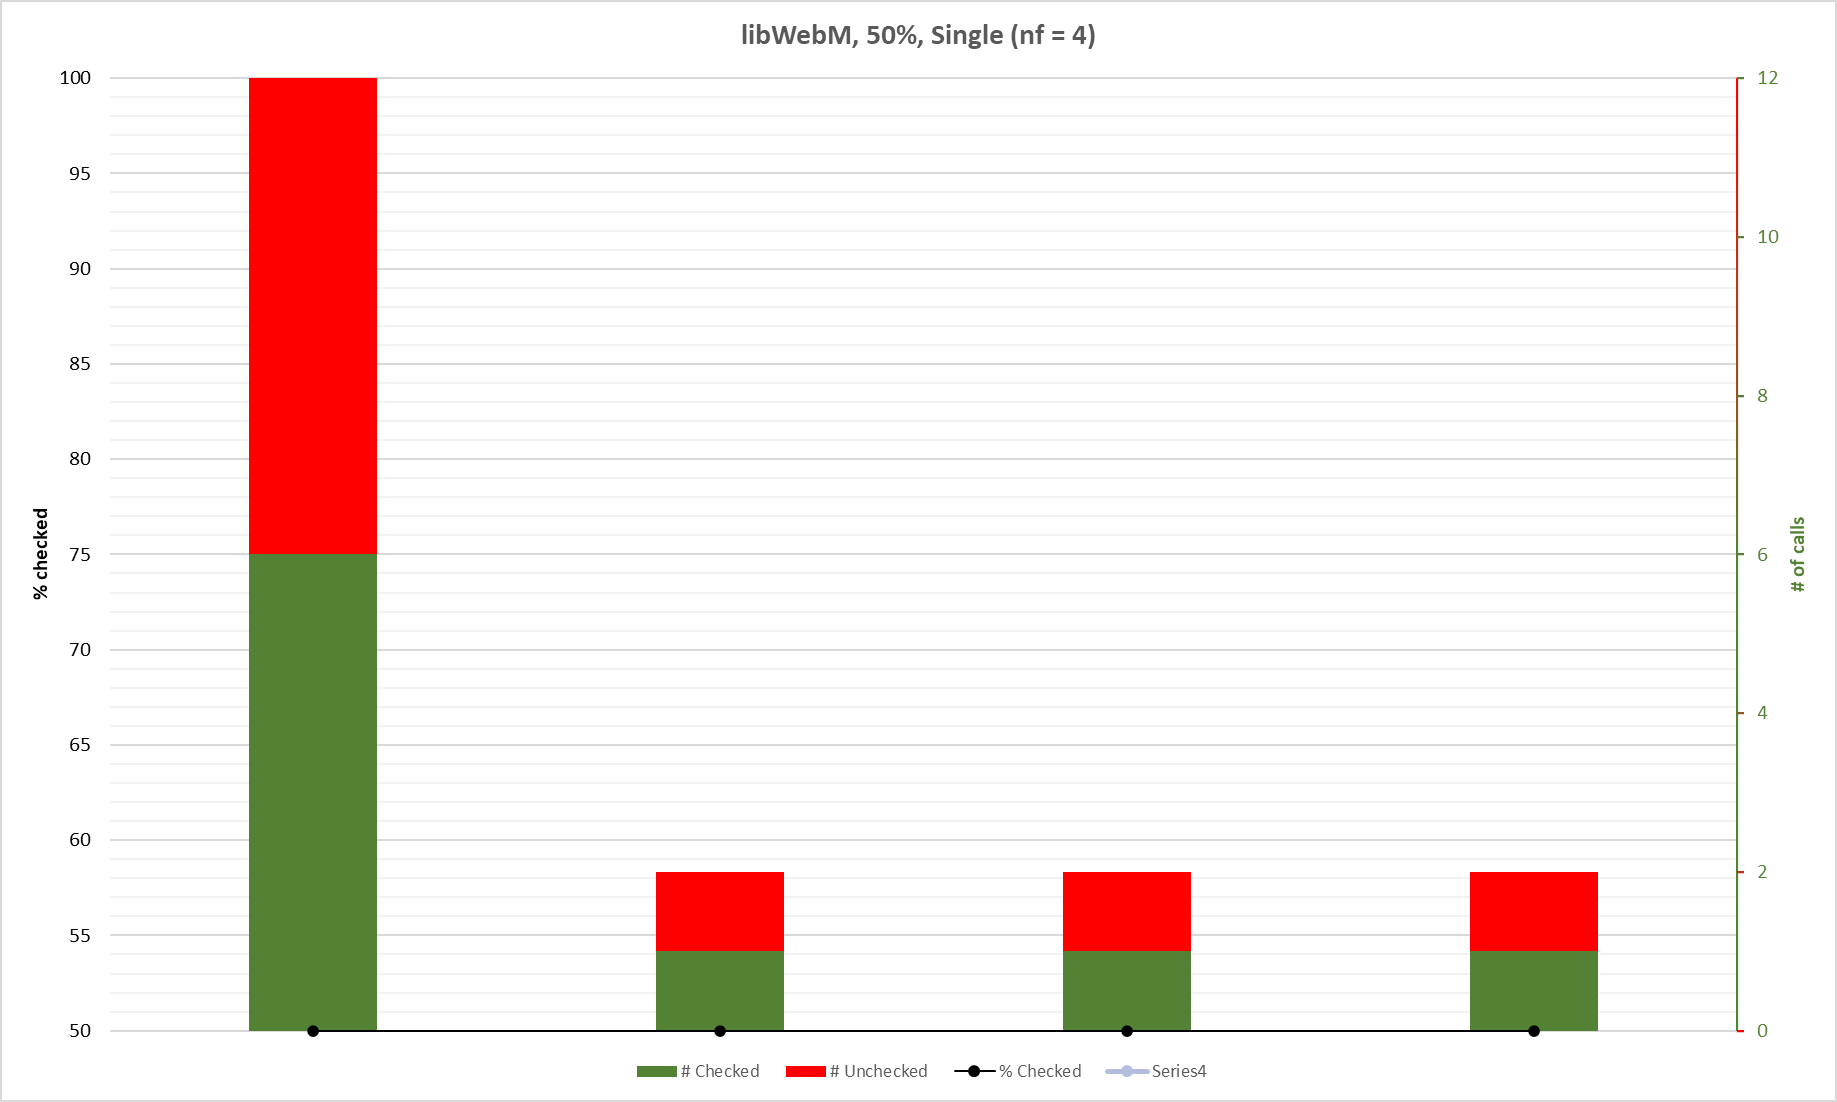
\includegraphics[width=1.2\linewidth]{images/appendix/libWebM_50_1_Single.png}}
\end{figure}

\begin{figure}[H]
	\makebox[\textwidth]{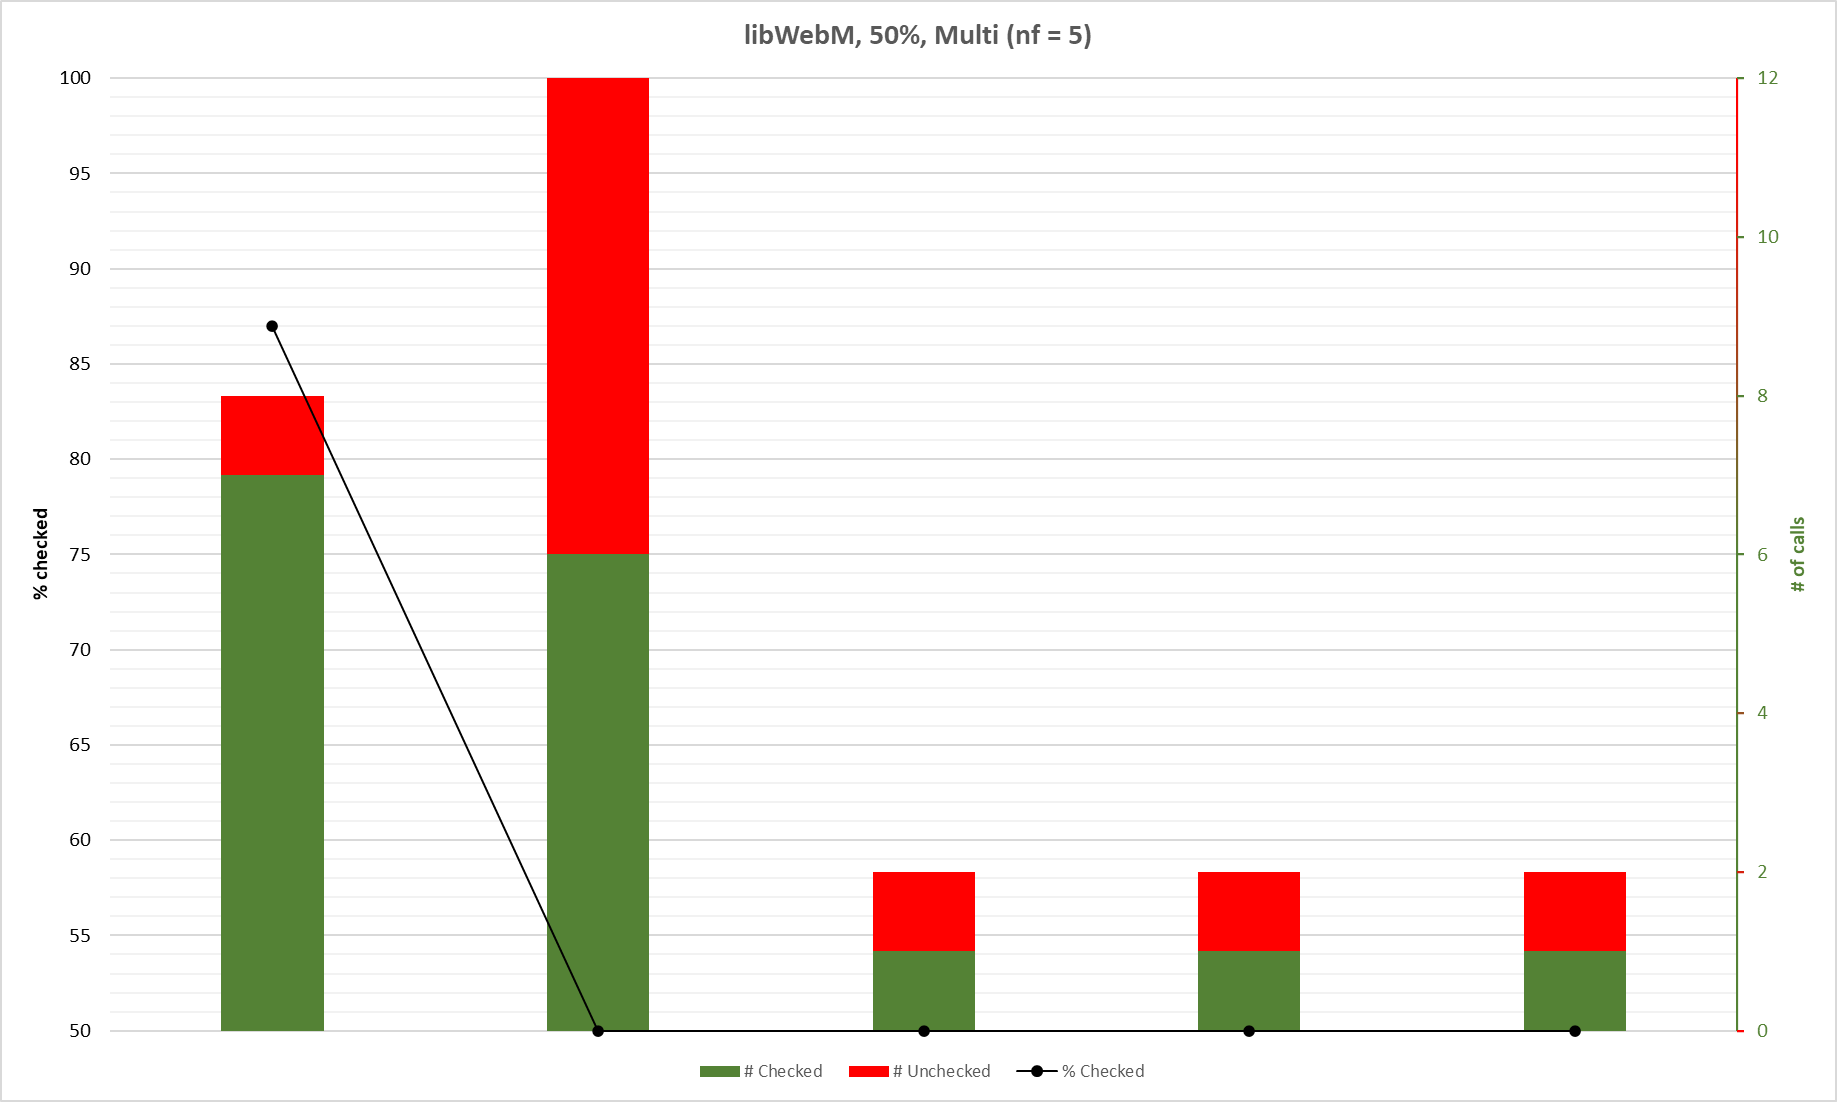
\includegraphics[width=1.2\linewidth]{images/appendix/libWebM_50_2_Multi.png}}
\end{figure}

\begin{figure}[H]
	\makebox[\textwidth]{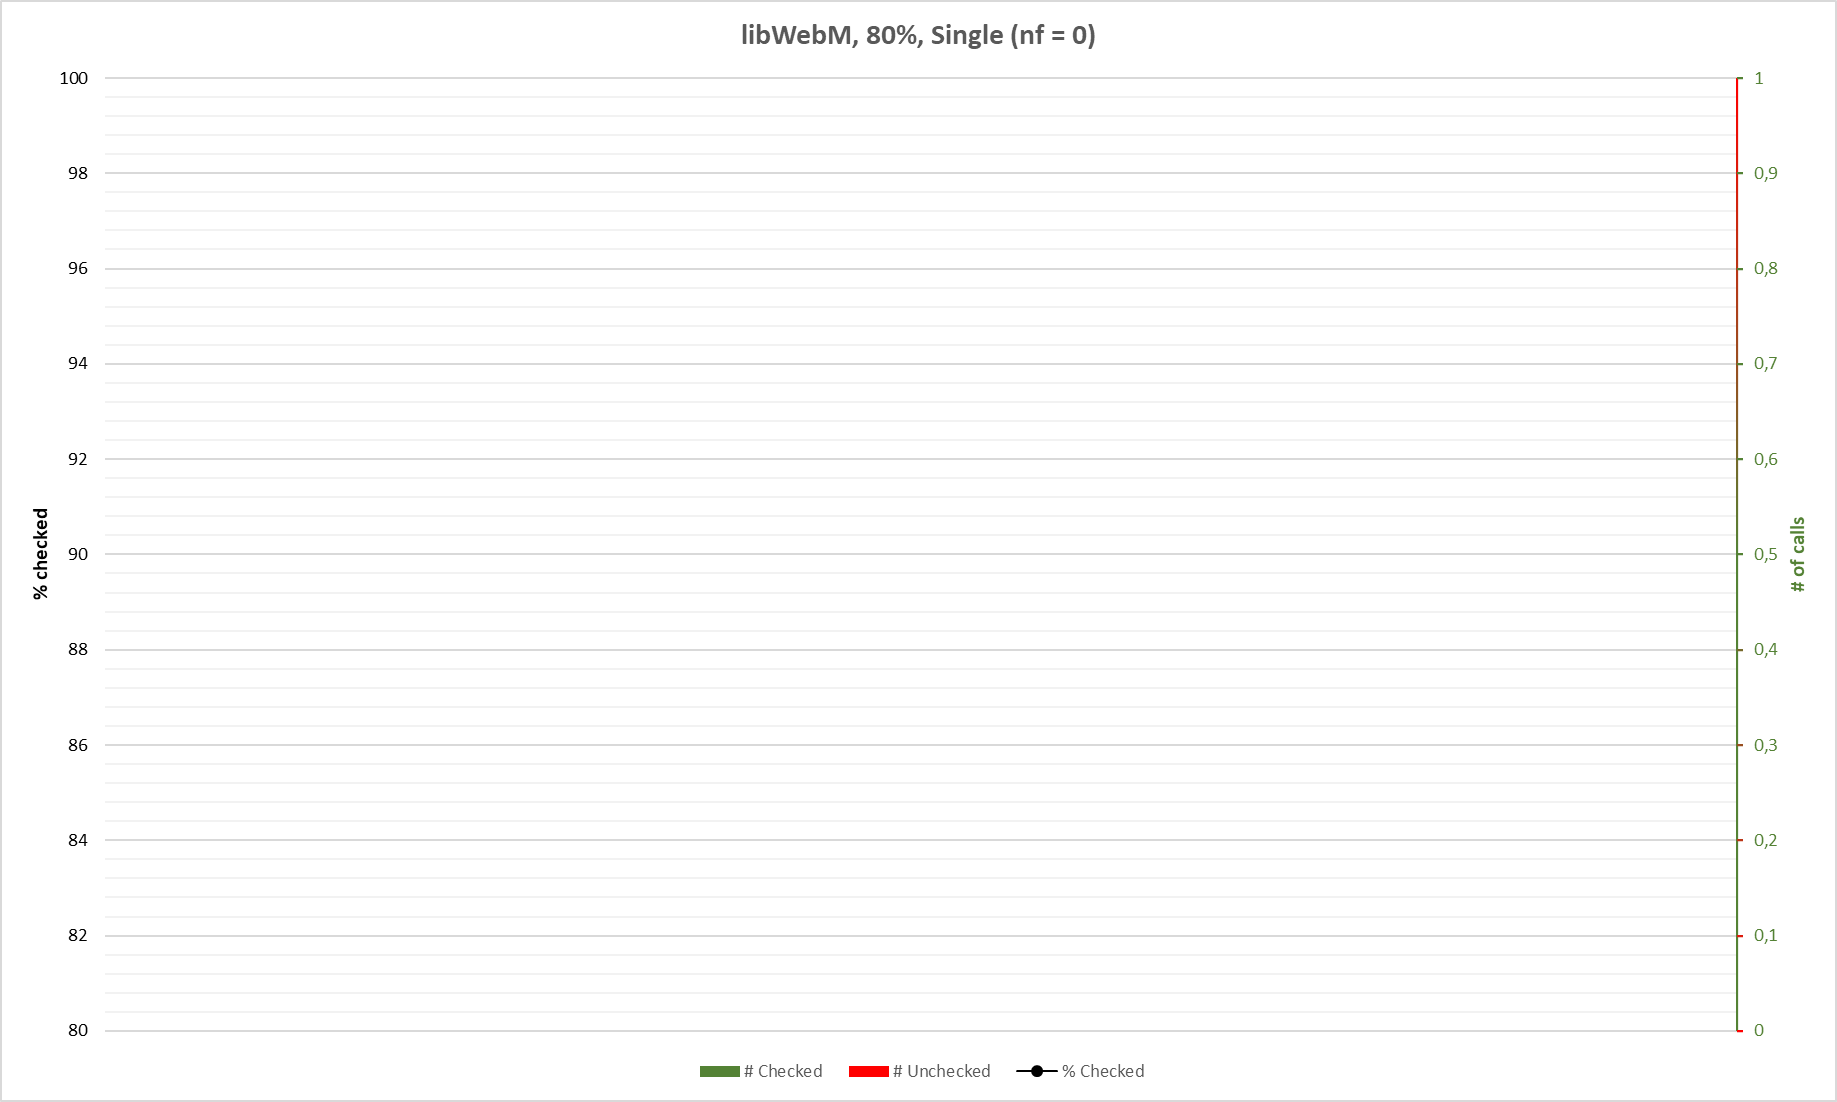
\includegraphics[width=1.2\linewidth]{images/appendix/libWebM_80_1_Single.png}}
\end{figure}

\begin{figure}[H]
	\makebox[\textwidth]{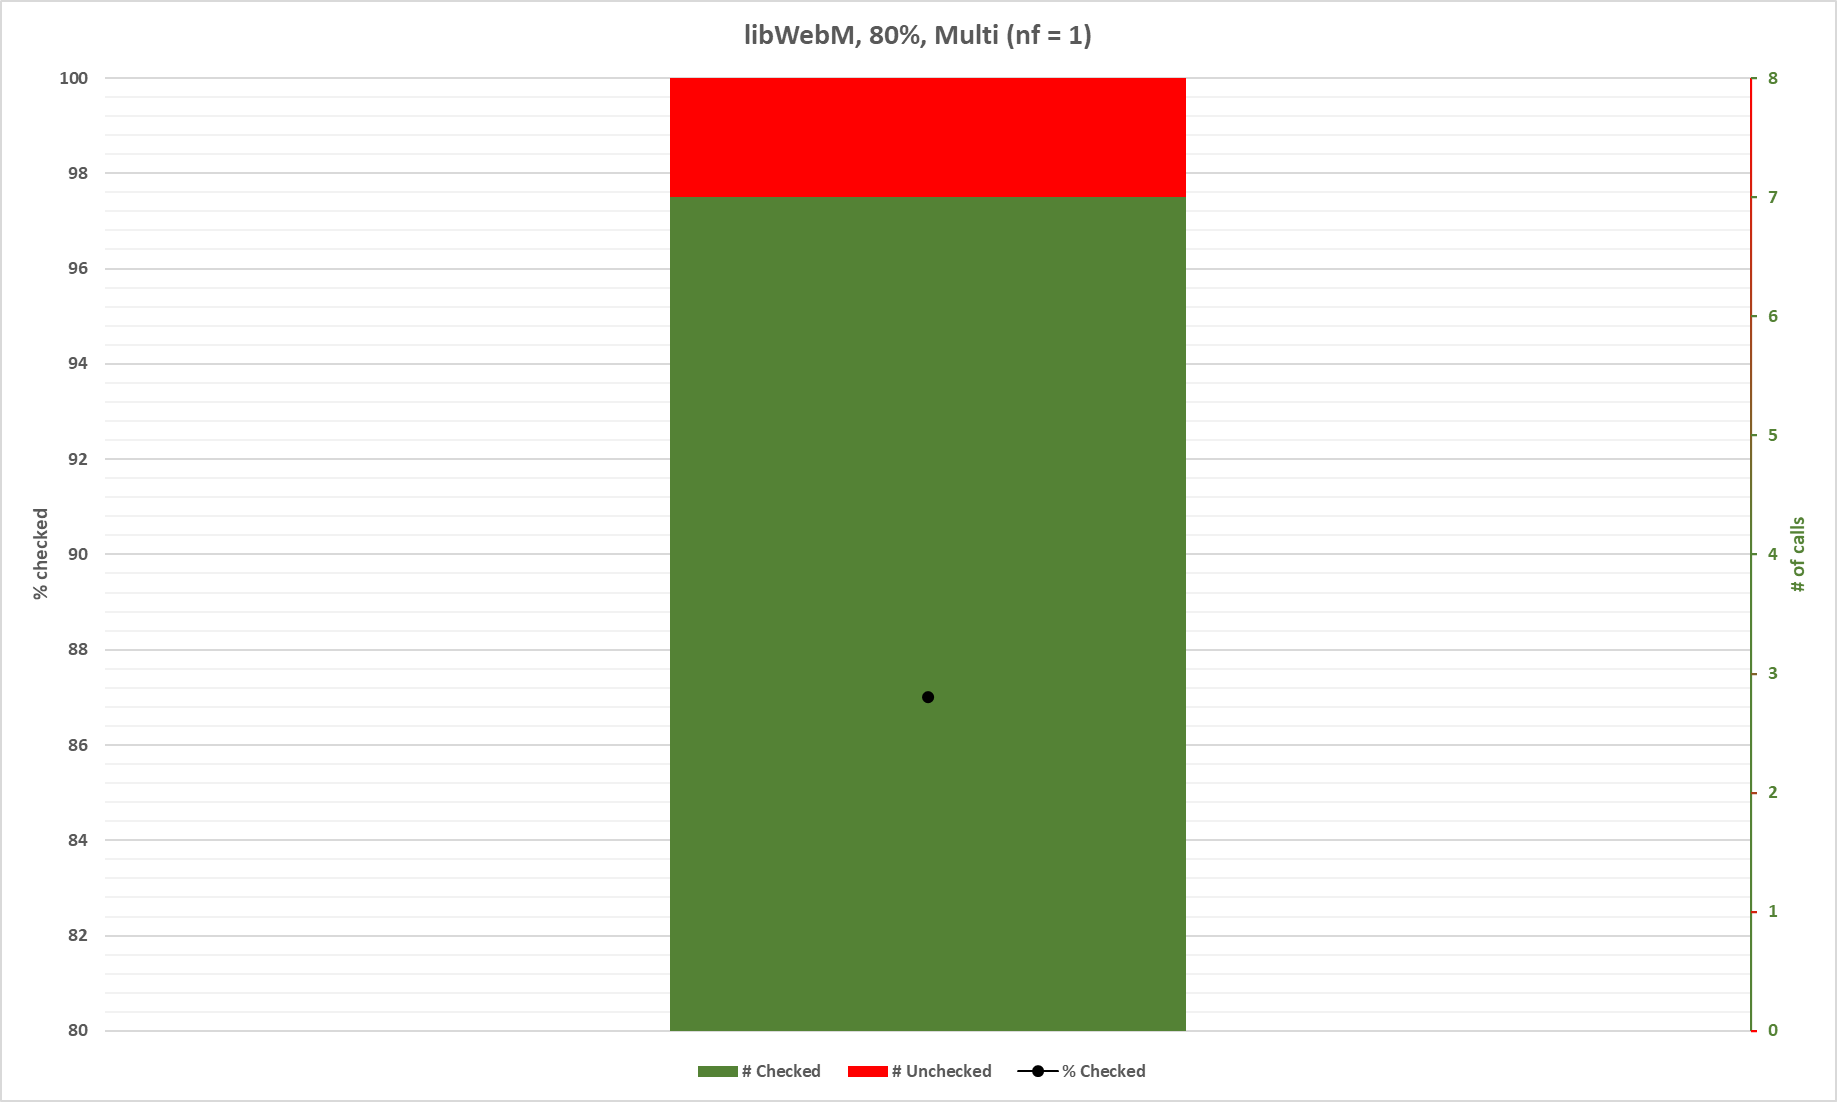
\includegraphics[width=1.2\linewidth]{images/appendix/libWebM_80_2_Multi.png}}
\end{figure}

\begin{figure}[H]
	\makebox[\textwidth]{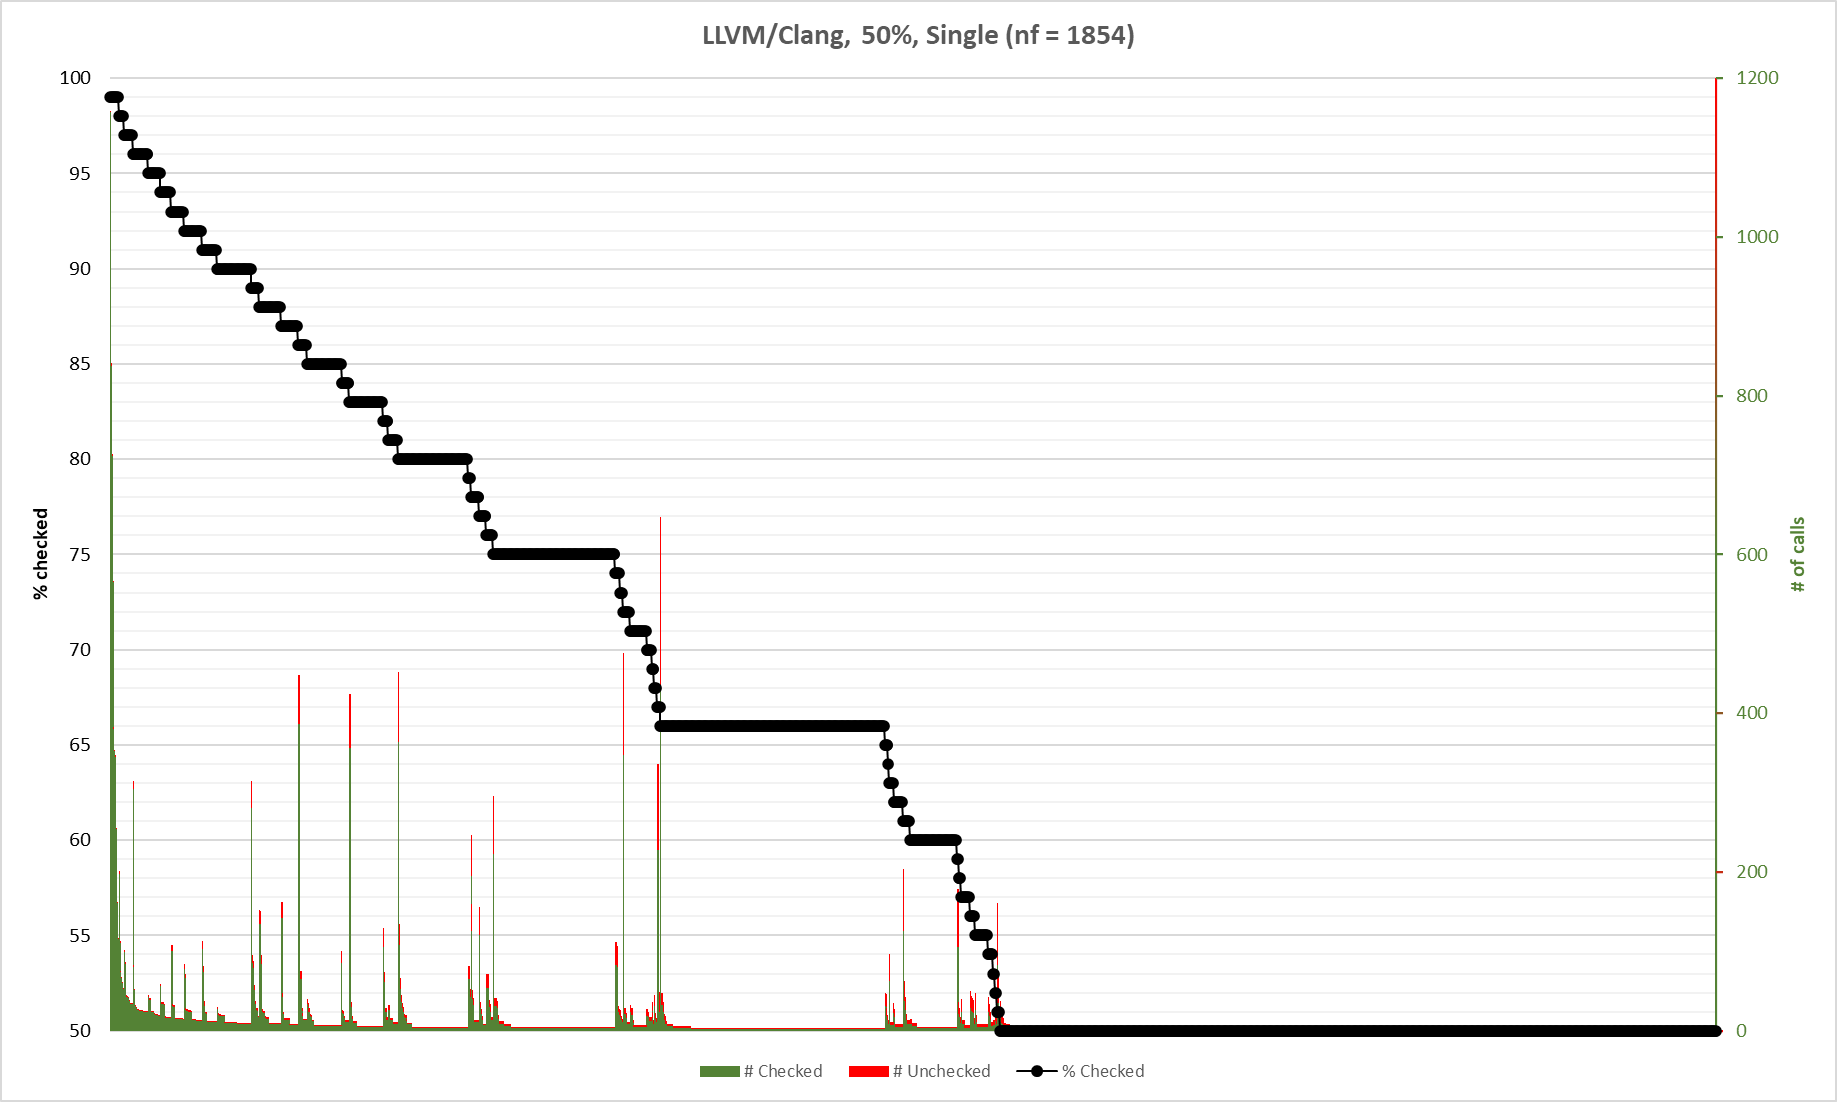
\includegraphics[width=1.2\linewidth]{images/appendix/LLVM_50_1_Single.png}}
\end{figure}

\begin{figure}[H]
	\makebox[\textwidth]{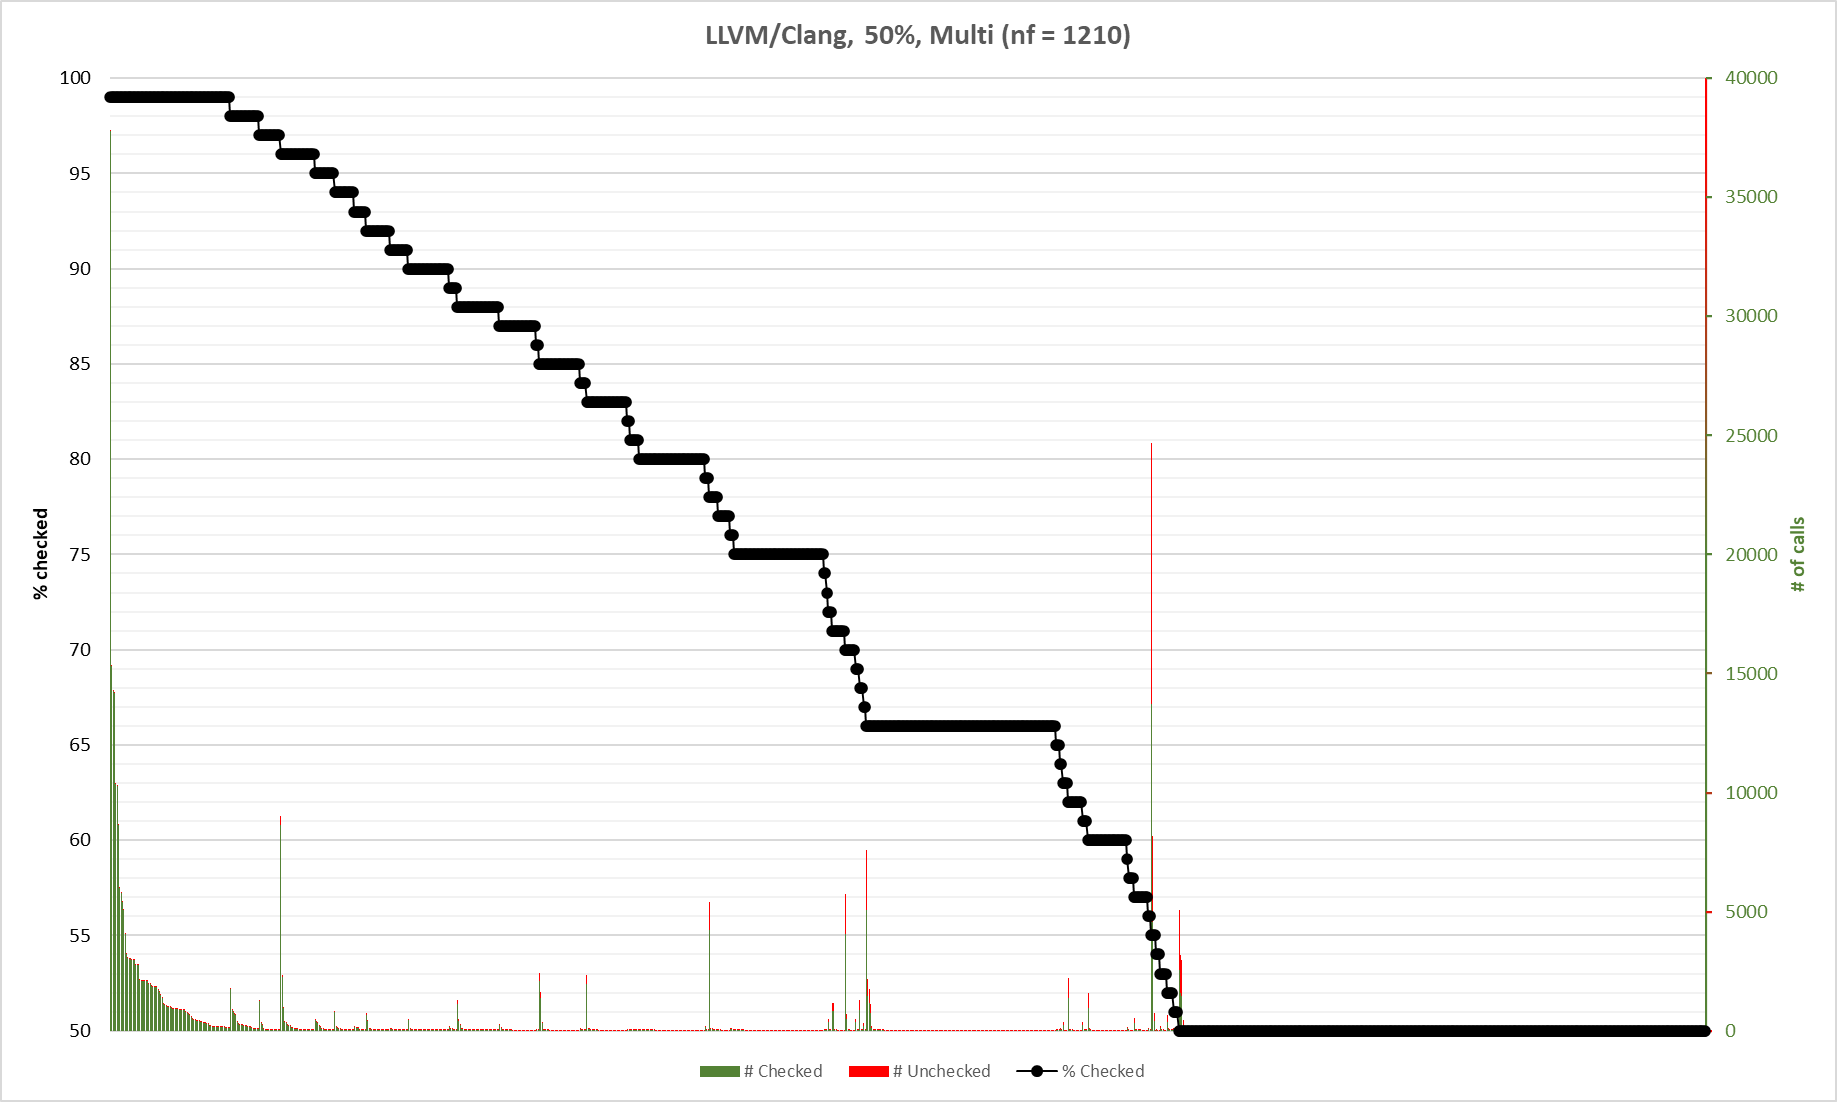
\includegraphics[width=1.2\linewidth]{images/appendix/LLVM_50_2_Multi.png}}
\end{figure}

\begin{figure}[H]
	\makebox[\textwidth]{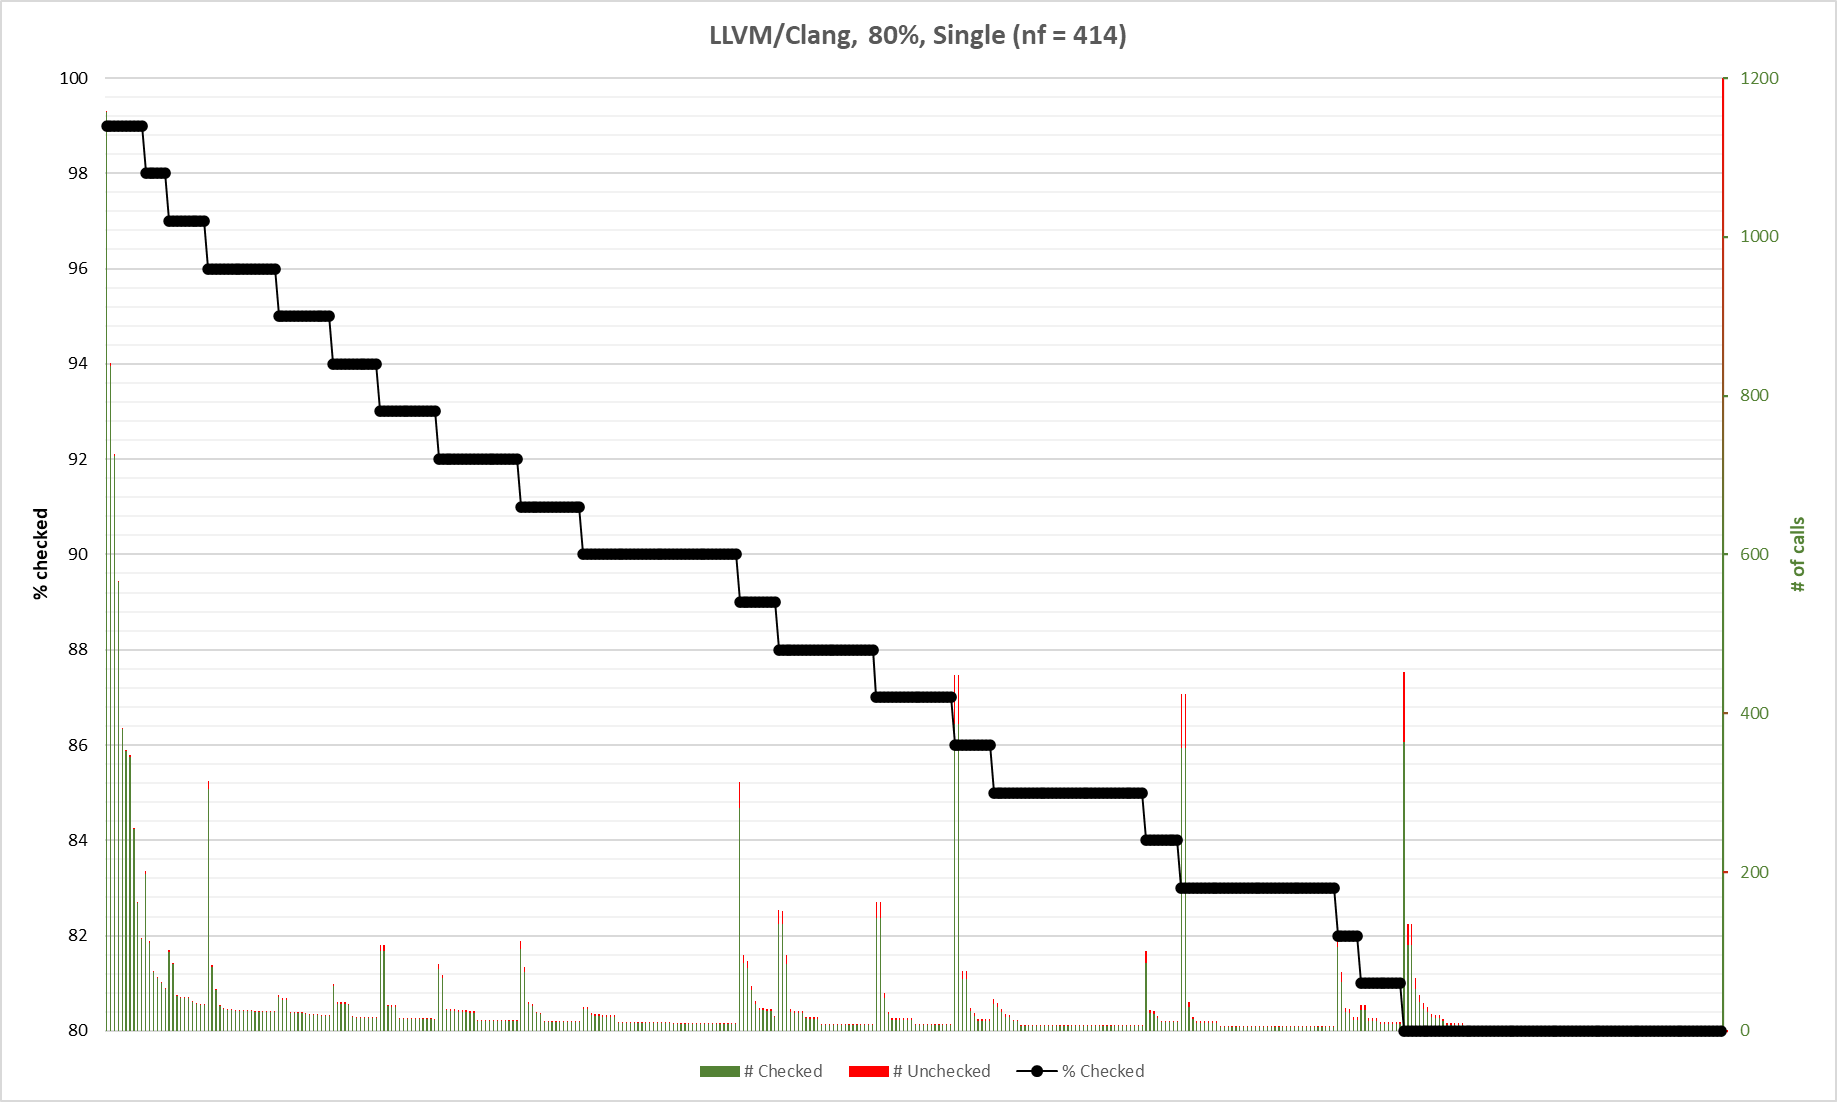
\includegraphics[width=1.2\linewidth]{images/appendix/LLVM_80_1_Single.png}}
\end{figure}

\begin{figure}[H]
	\makebox[\textwidth]{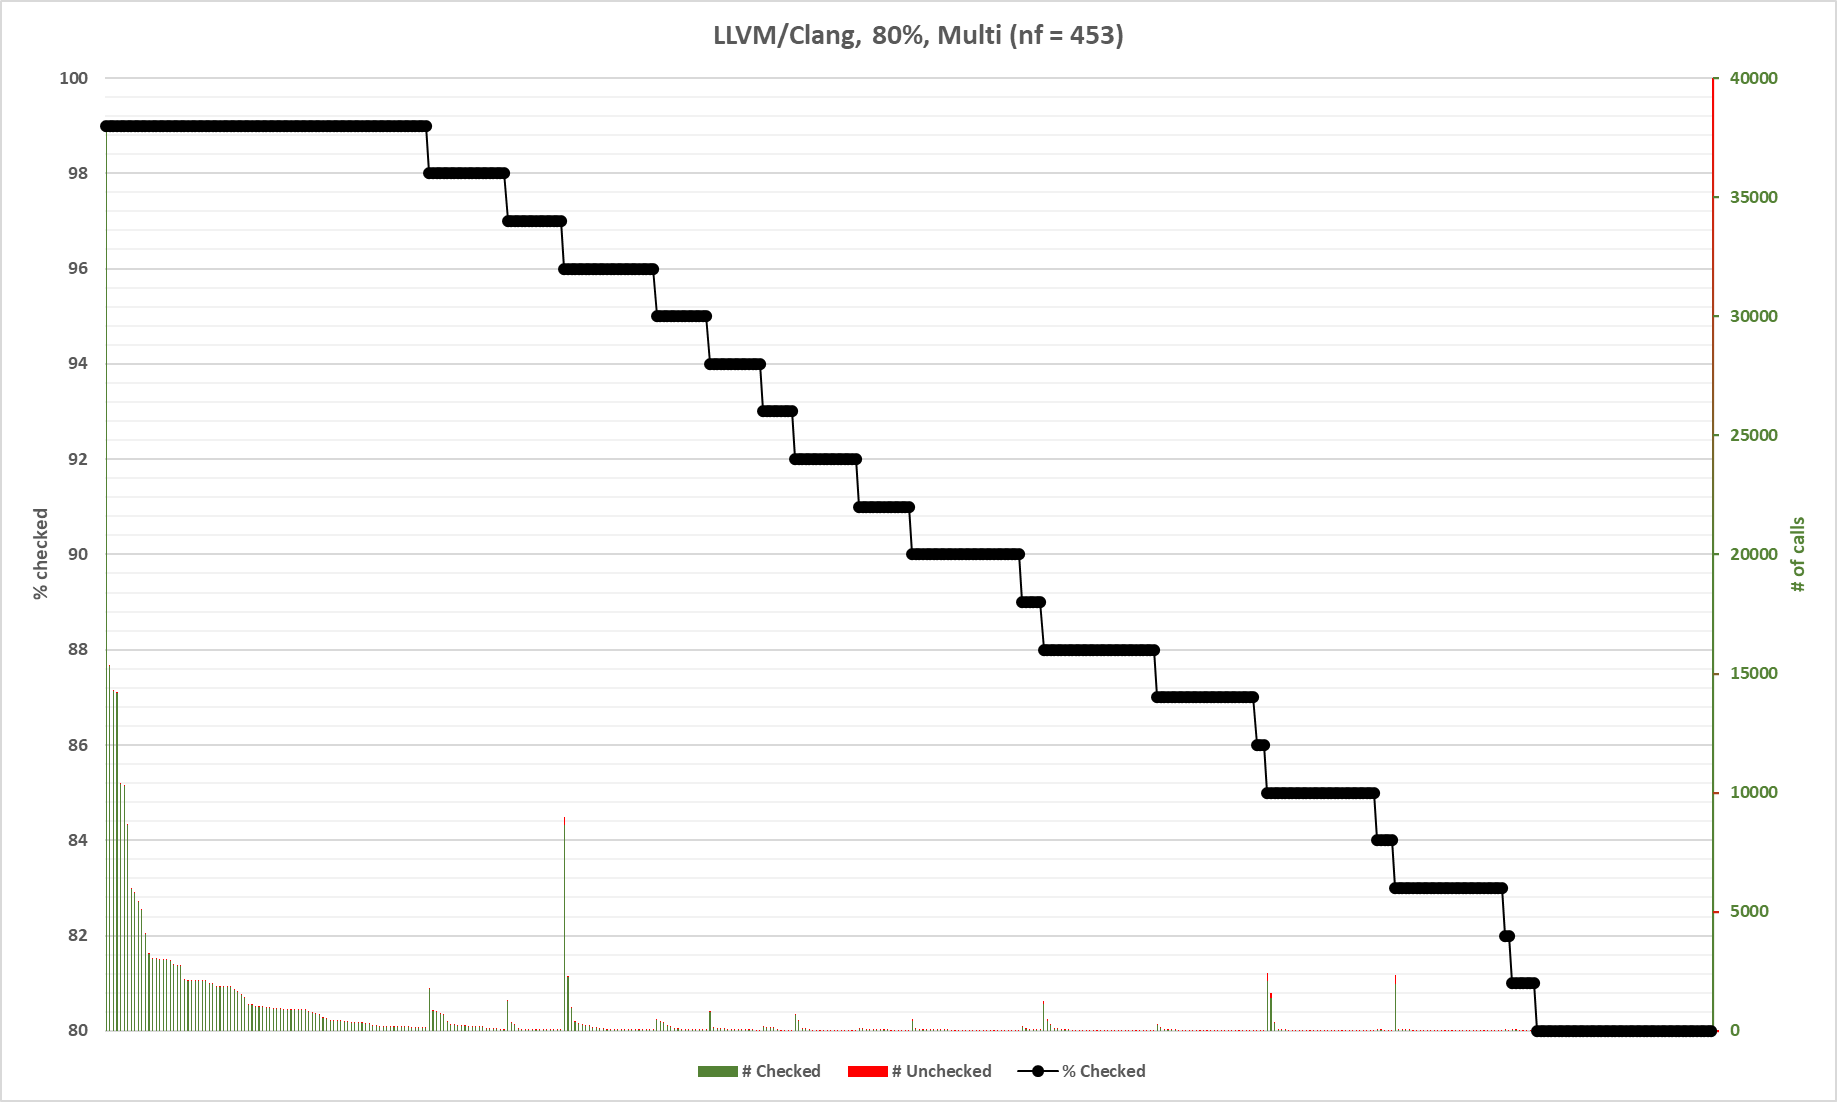
\includegraphics[width=1.2\linewidth]{images/appendix/LLVM_80_2_Multi.png}}
\end{figure}

\begin{figure}[H]
	\makebox[\textwidth]{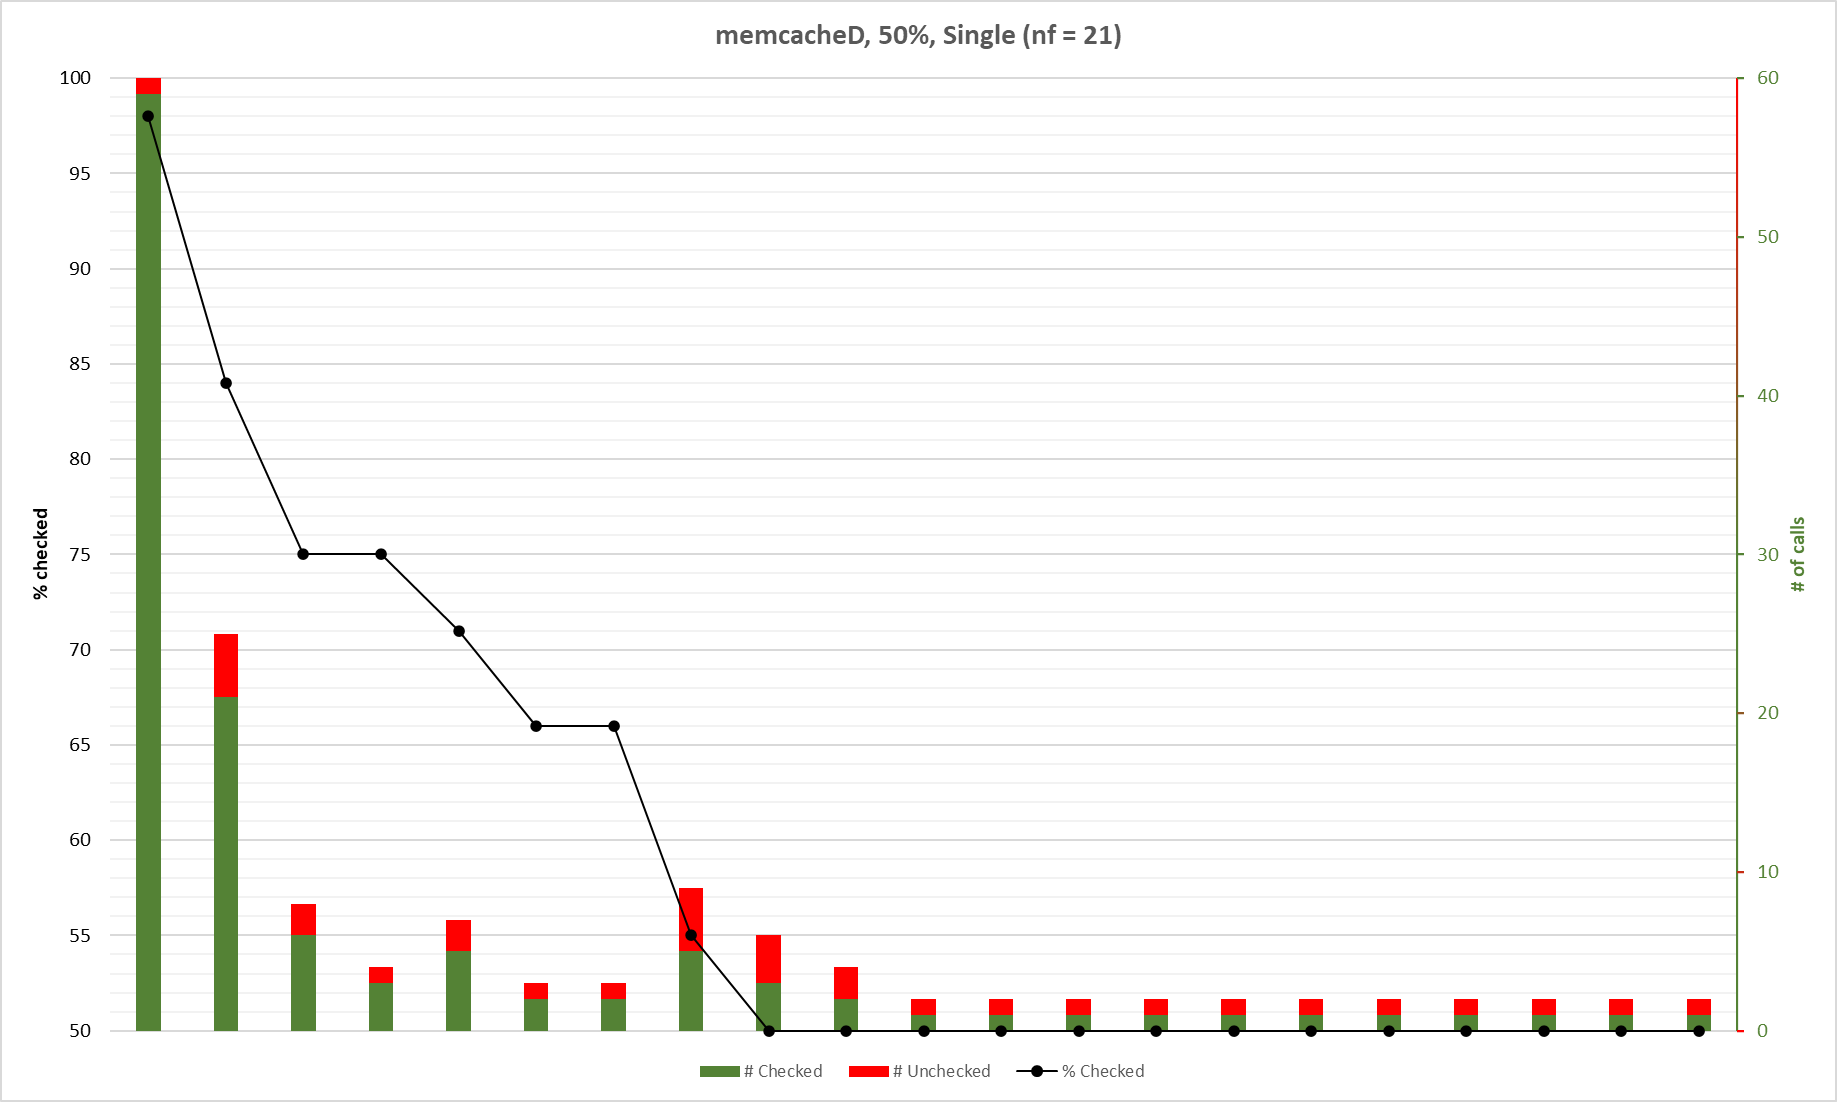
\includegraphics[width=1.2\linewidth]{images/appendix/memcacheD_50_1_Single.png}}
\end{figure}

\begin{figure}[H]
	\makebox[\textwidth]{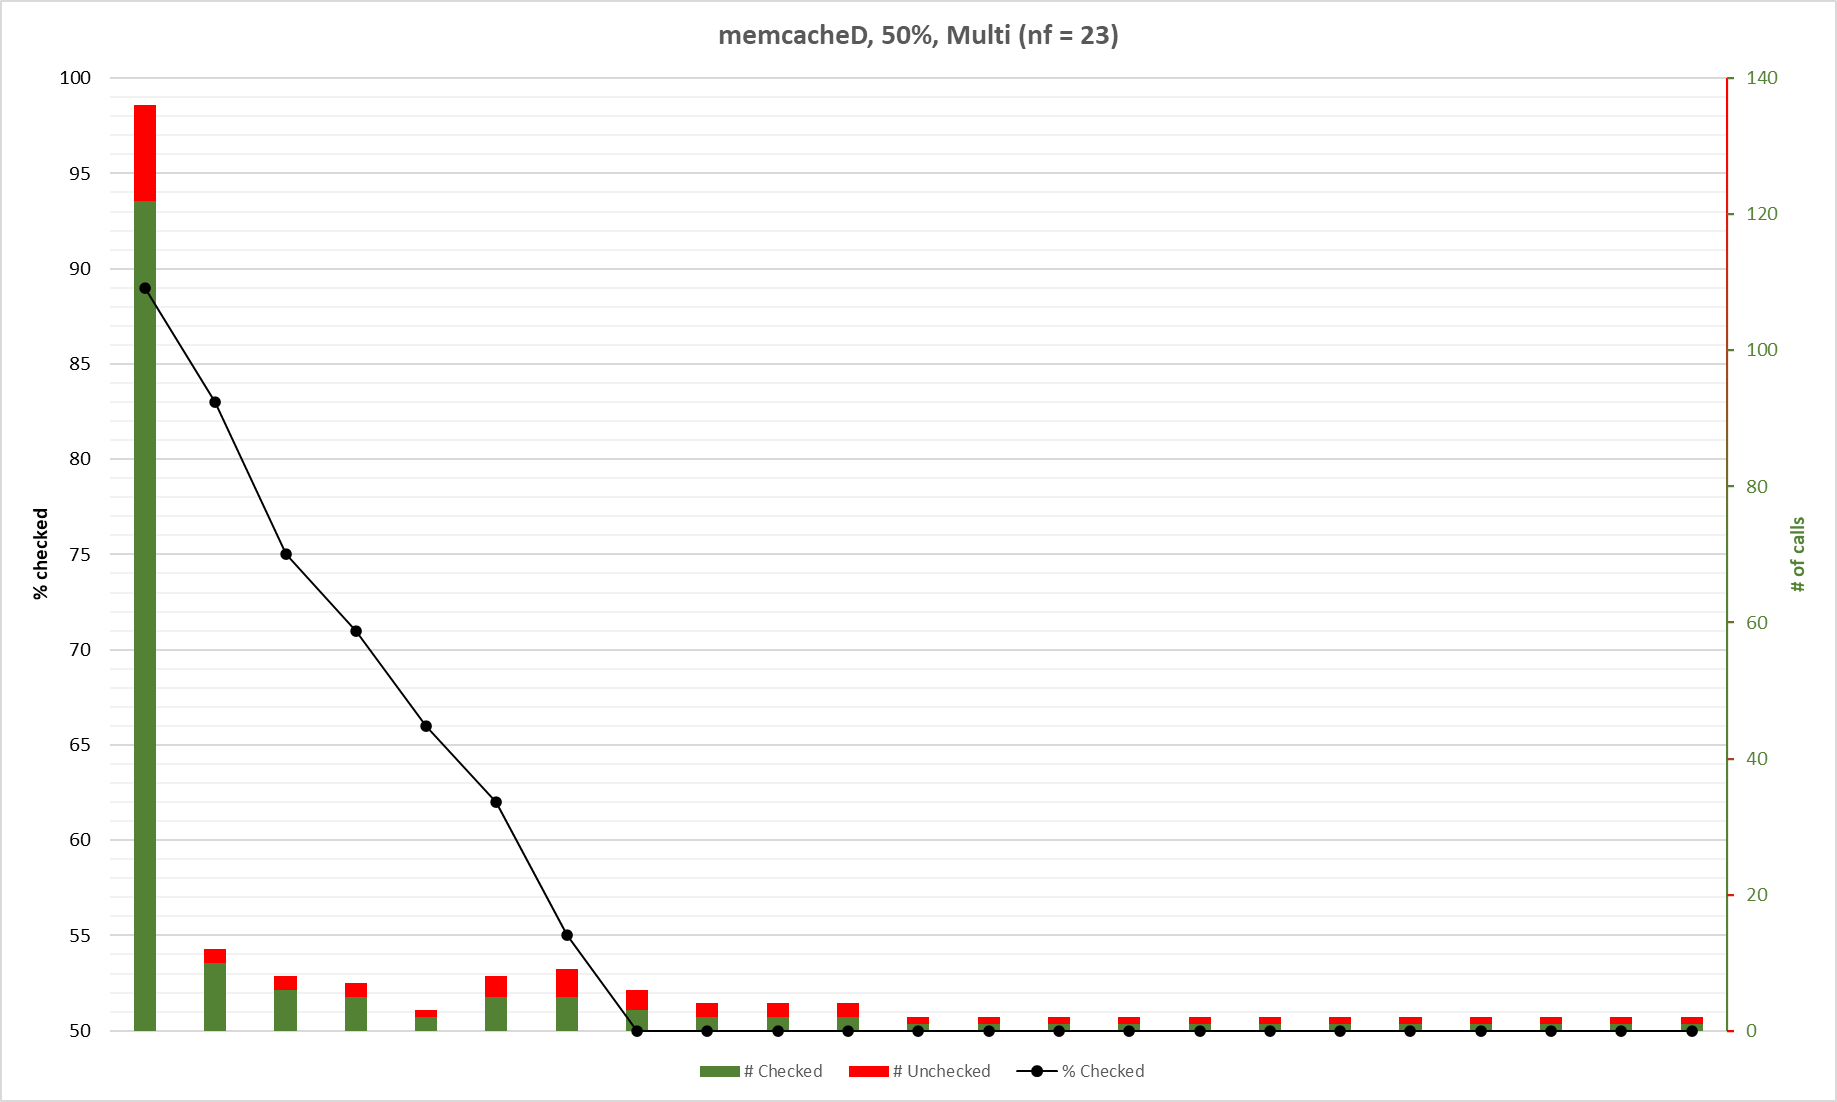
\includegraphics[width=1.2\linewidth]{images/appendix/memcacheD_50_2_Multi.png}}
\end{figure}

\begin{figure}[H]
	\makebox[\textwidth]{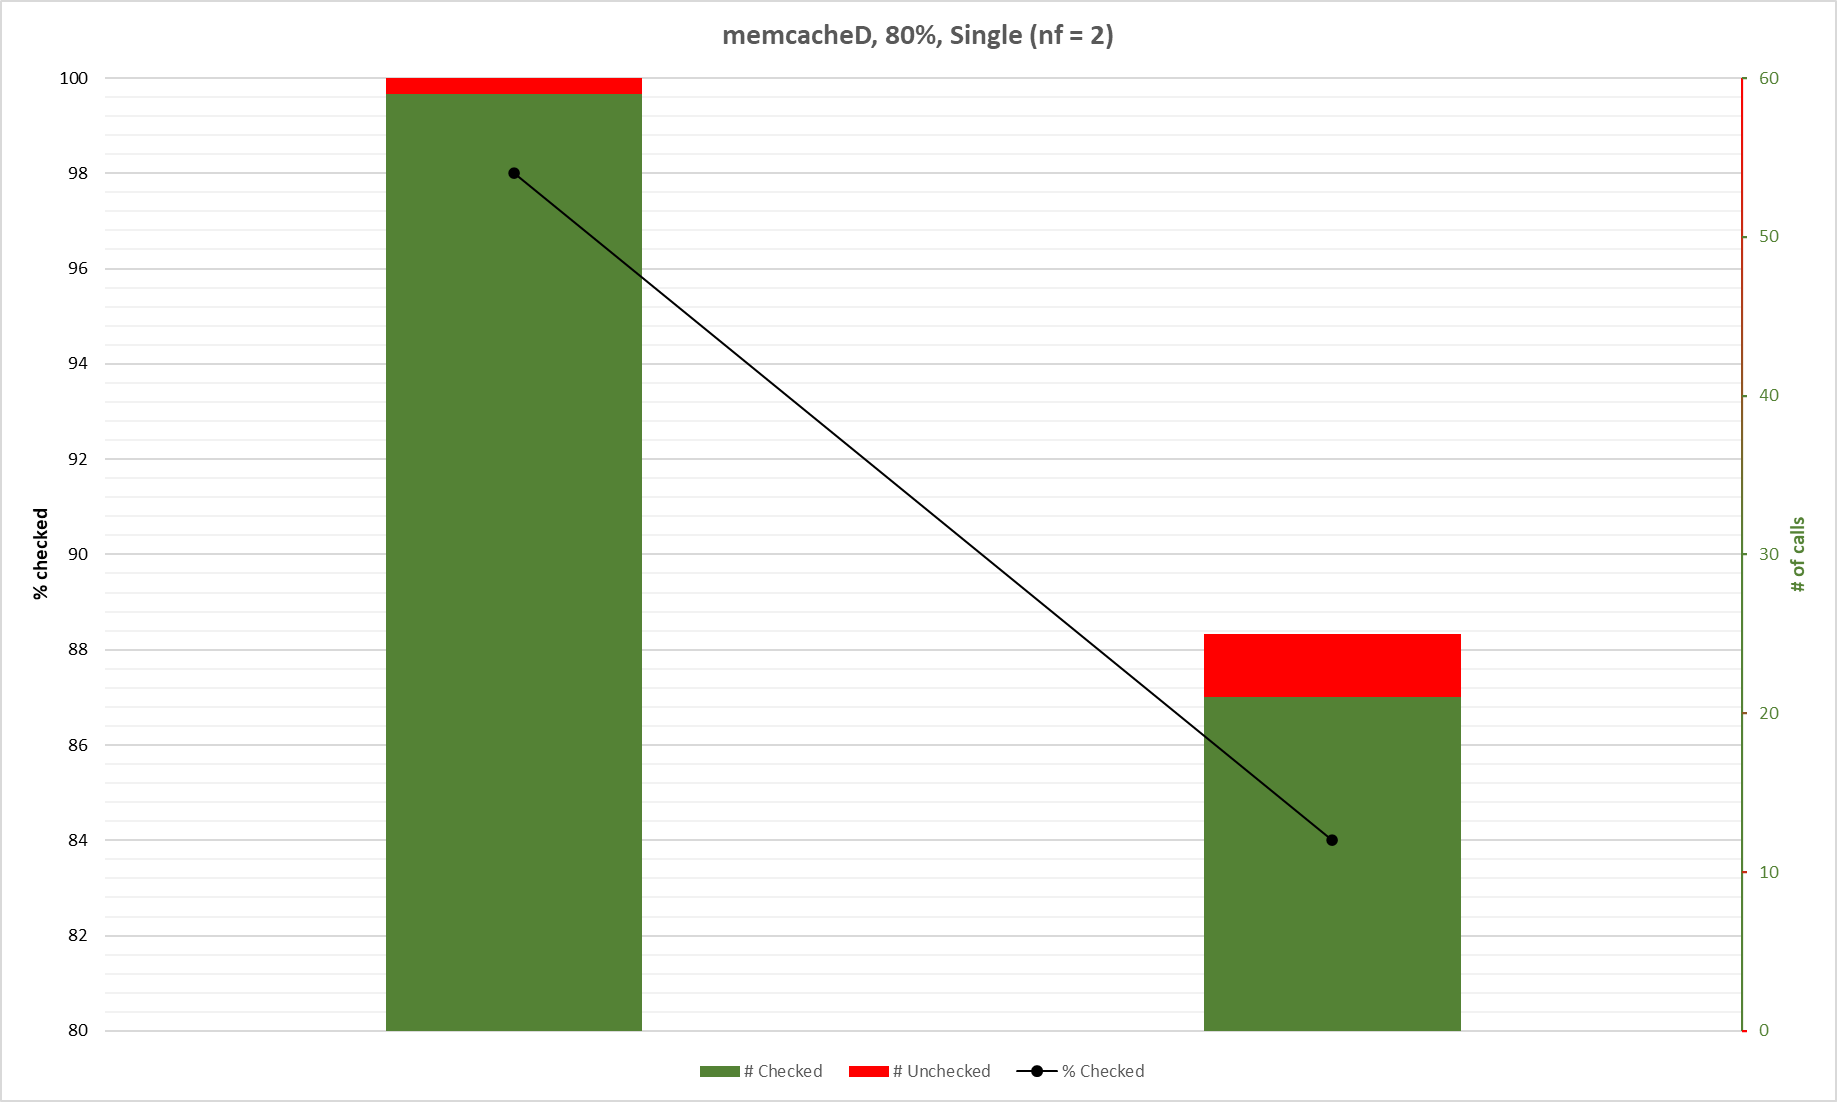
\includegraphics[width=1.2\linewidth]{images/appendix/memcacheD_80_1_Single.png}}
\end{figure}

\begin{figure}[H]
	\makebox[\textwidth]{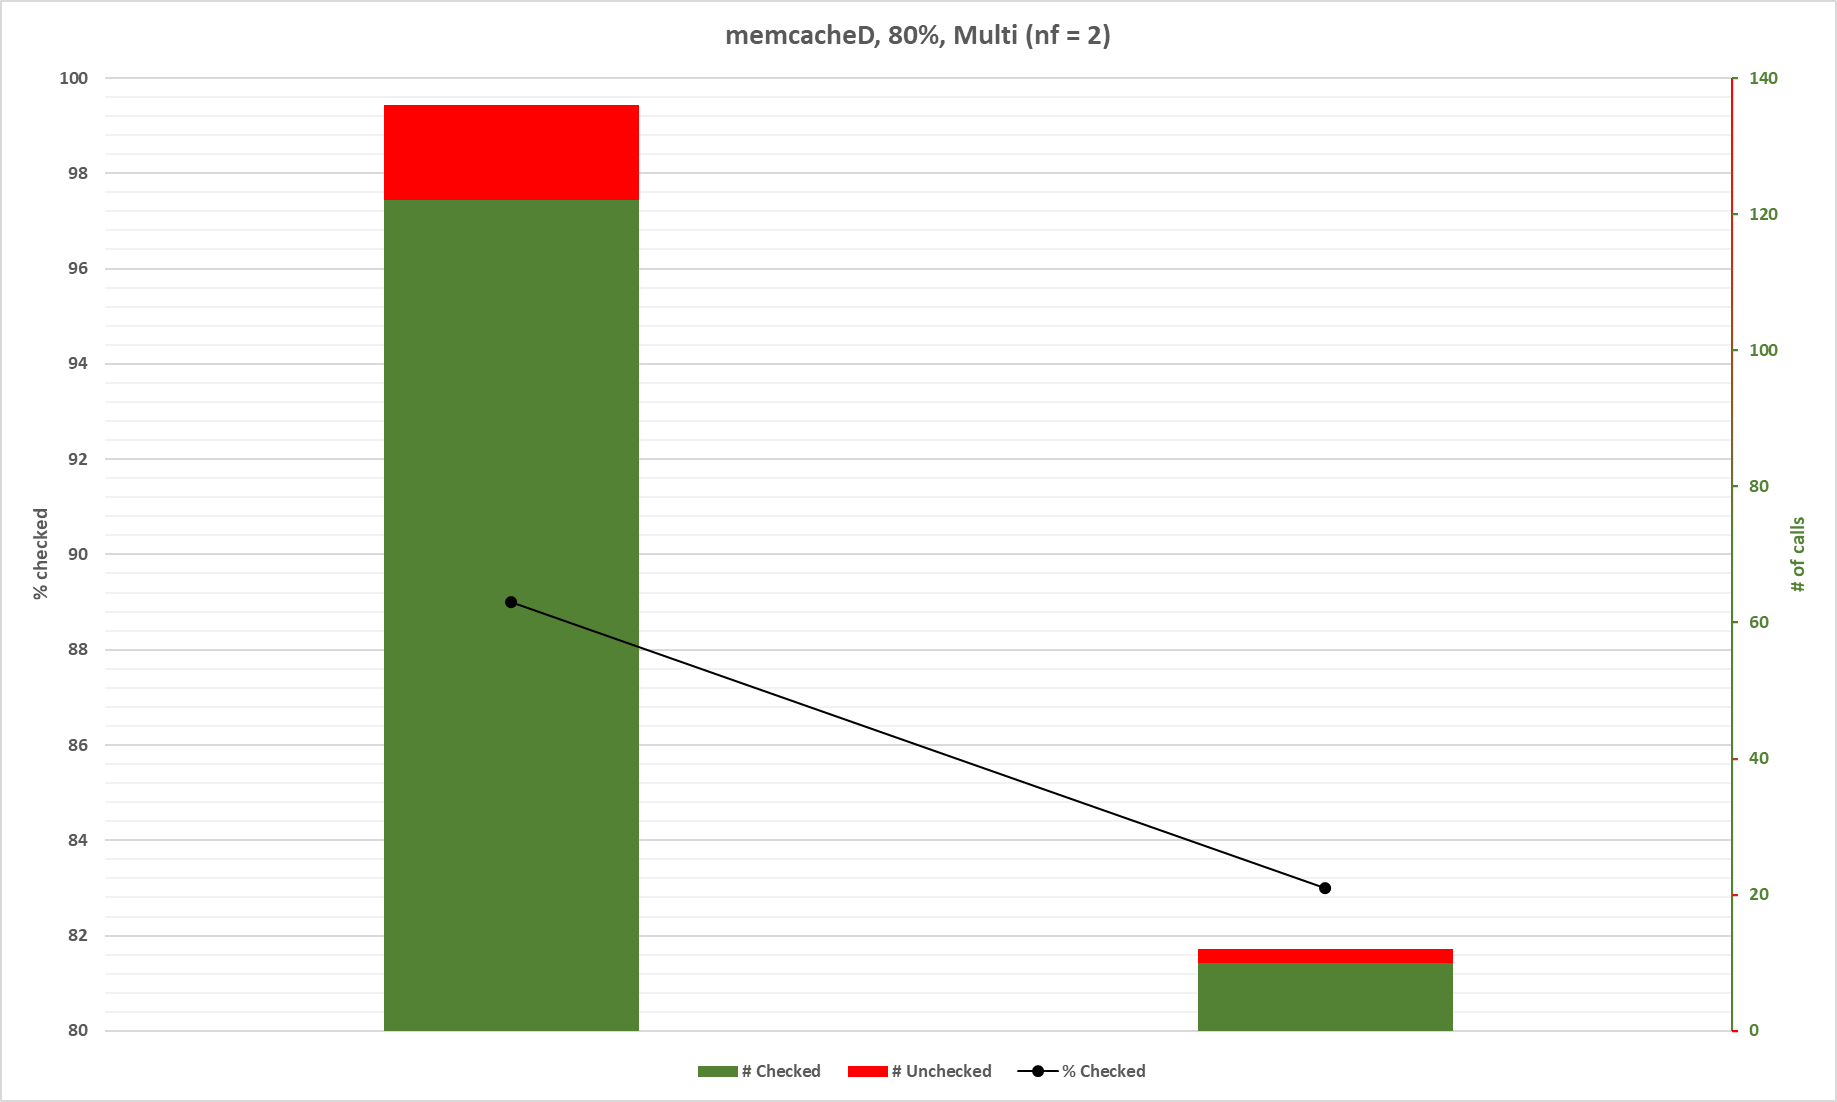
\includegraphics[width=1.2\linewidth]{images/appendix/memcacheD_80_2_Multi.png}}
\end{figure}

\begin{figure}[H]
	\makebox[\textwidth]{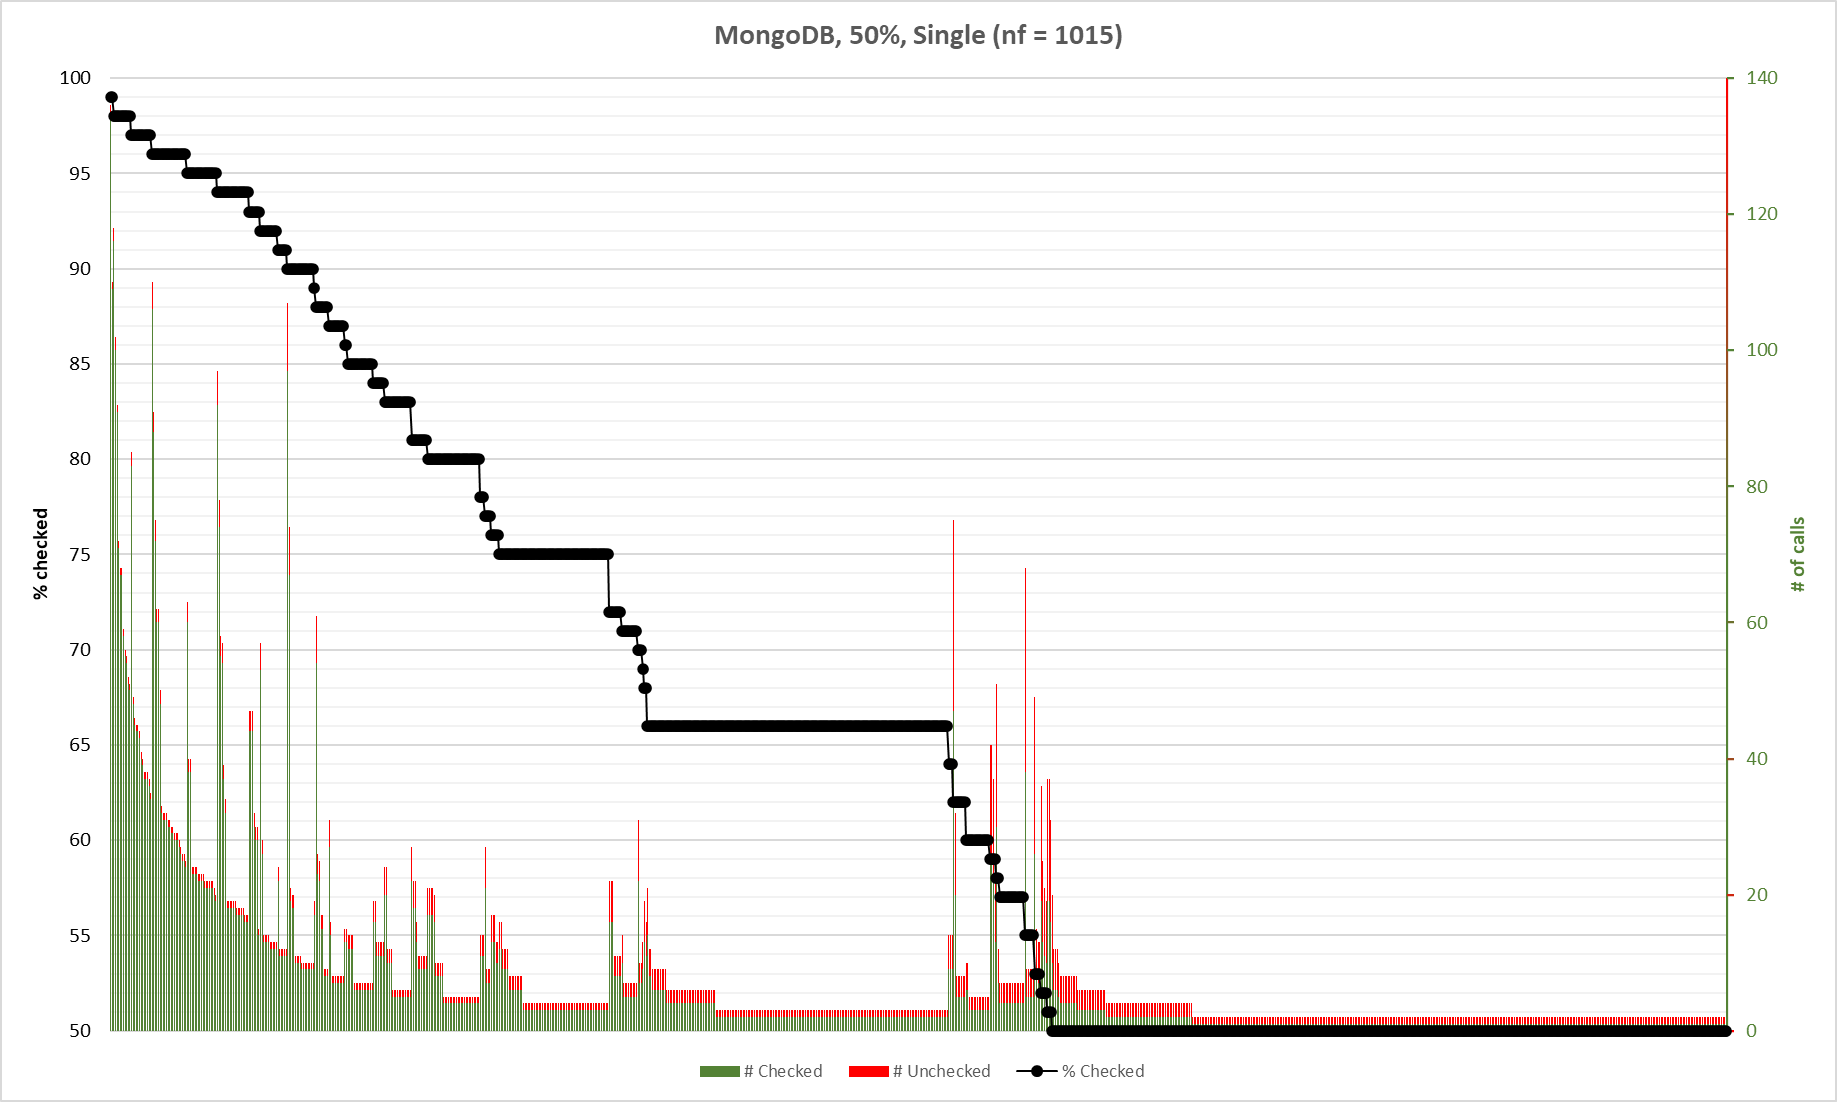
\includegraphics[width=1.2\linewidth]{images/appendix/MongoDB_50_1_Single.png}}
\end{figure}

\begin{figure}[H]
	\makebox[\textwidth]{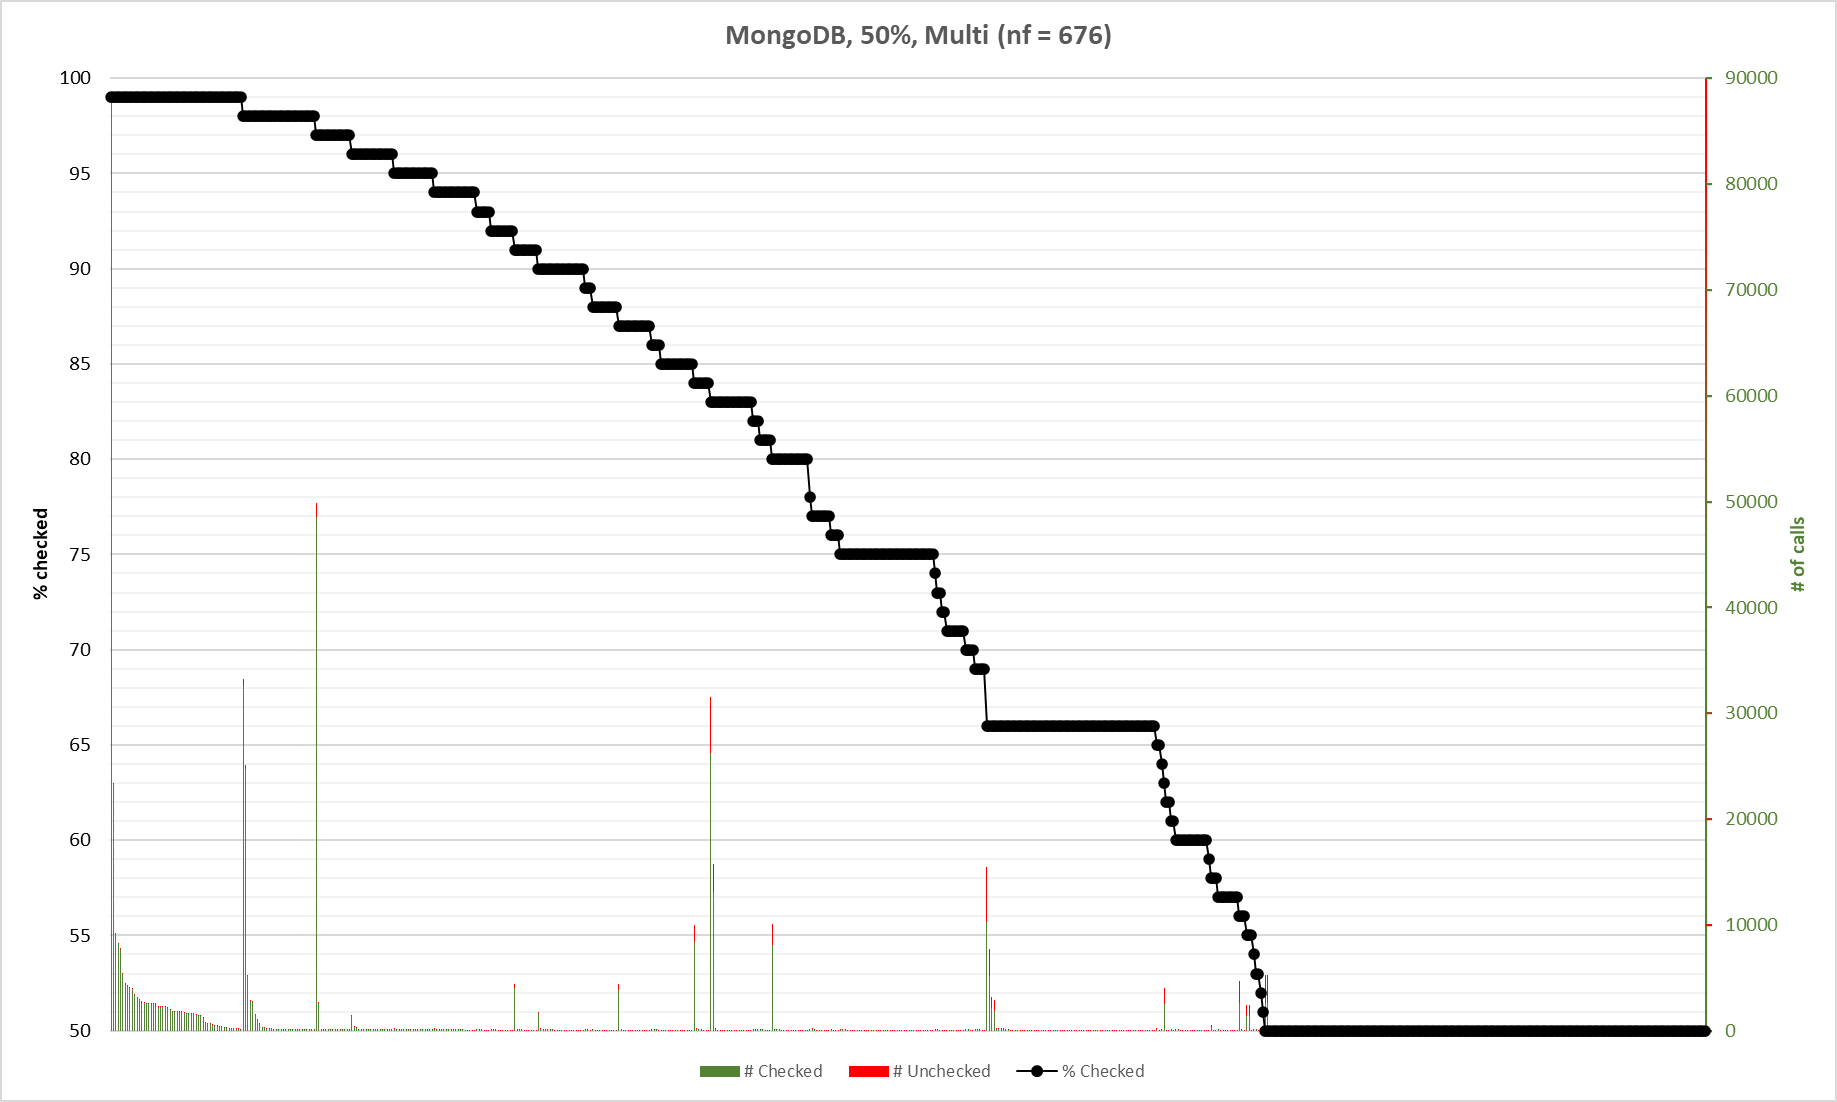
\includegraphics[width=1.2\linewidth]{images/appendix/MongoDB_50_2_Multi.png}}
\end{figure}

\begin{figure}[H]
	\makebox[\textwidth]{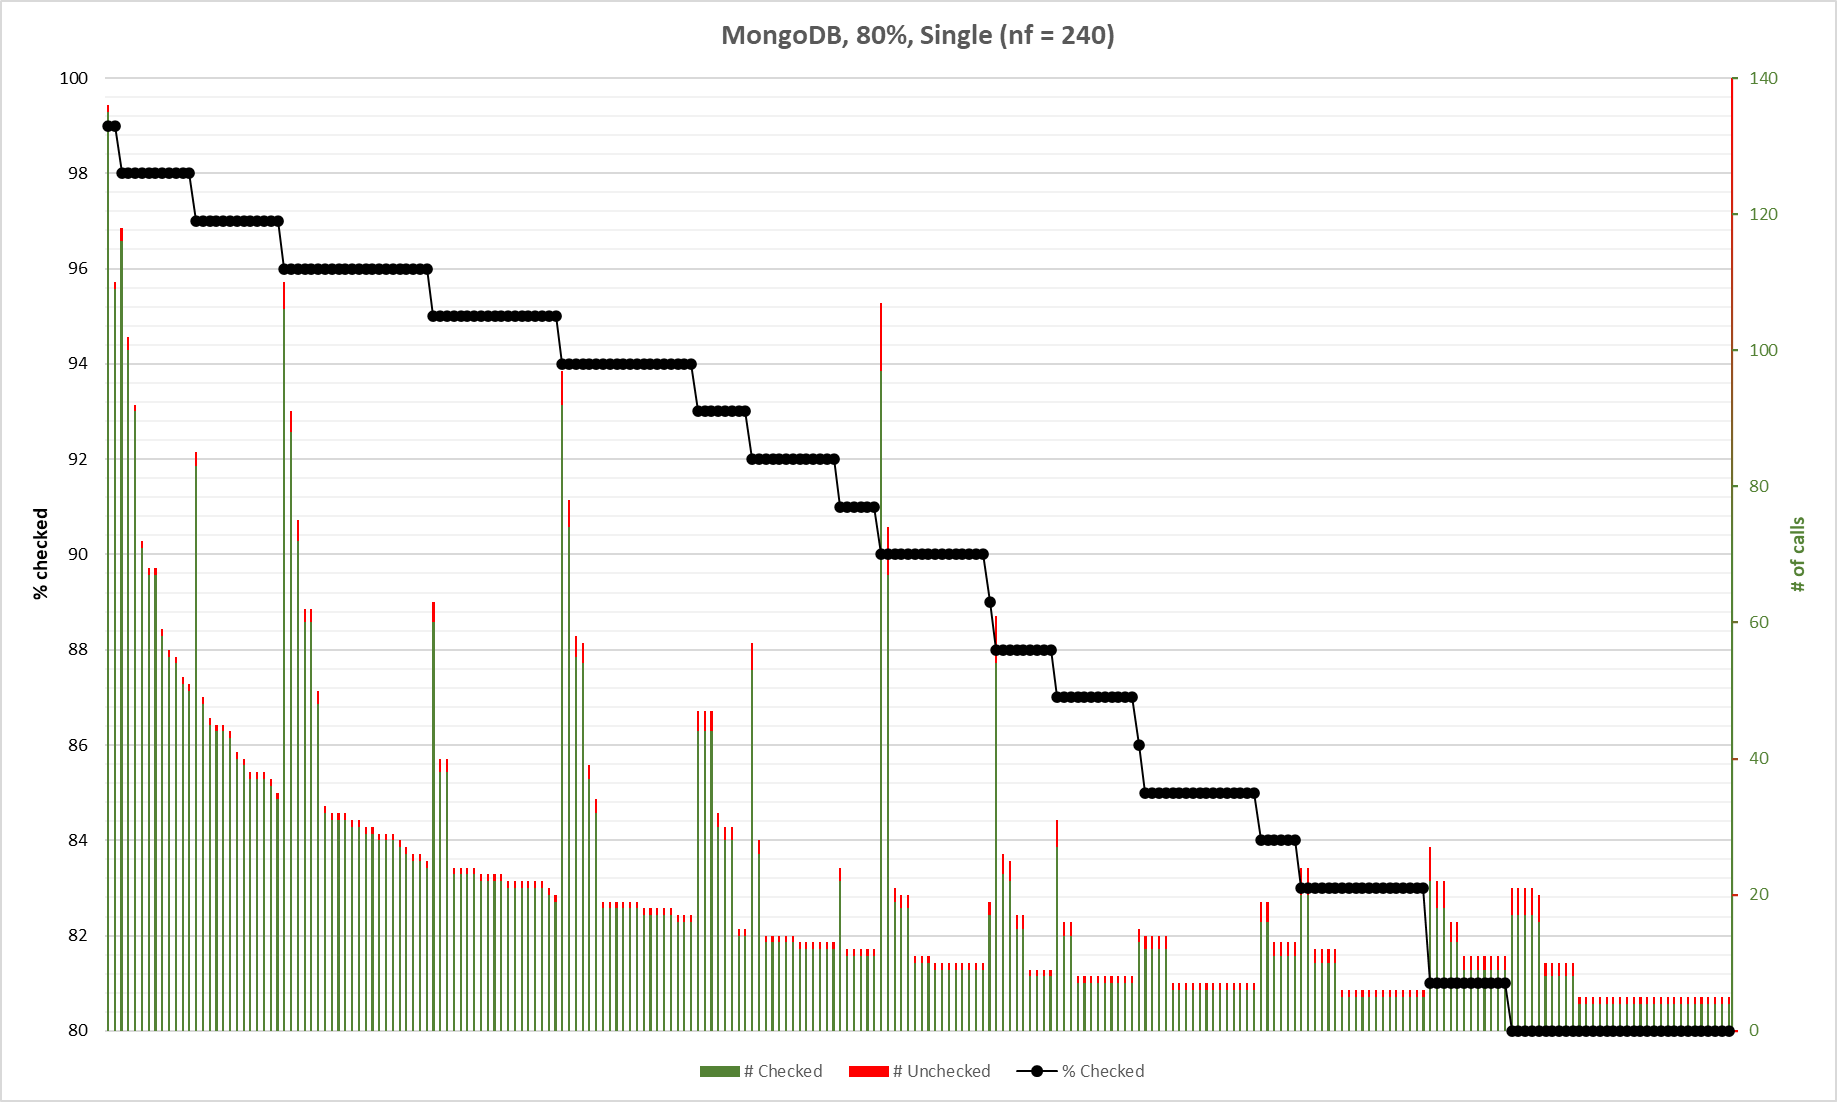
\includegraphics[width=1.2\linewidth]{images/appendix/MongoDB_80_1_Single.png}}
\end{figure}

\begin{figure}[H]
	\makebox[\textwidth]{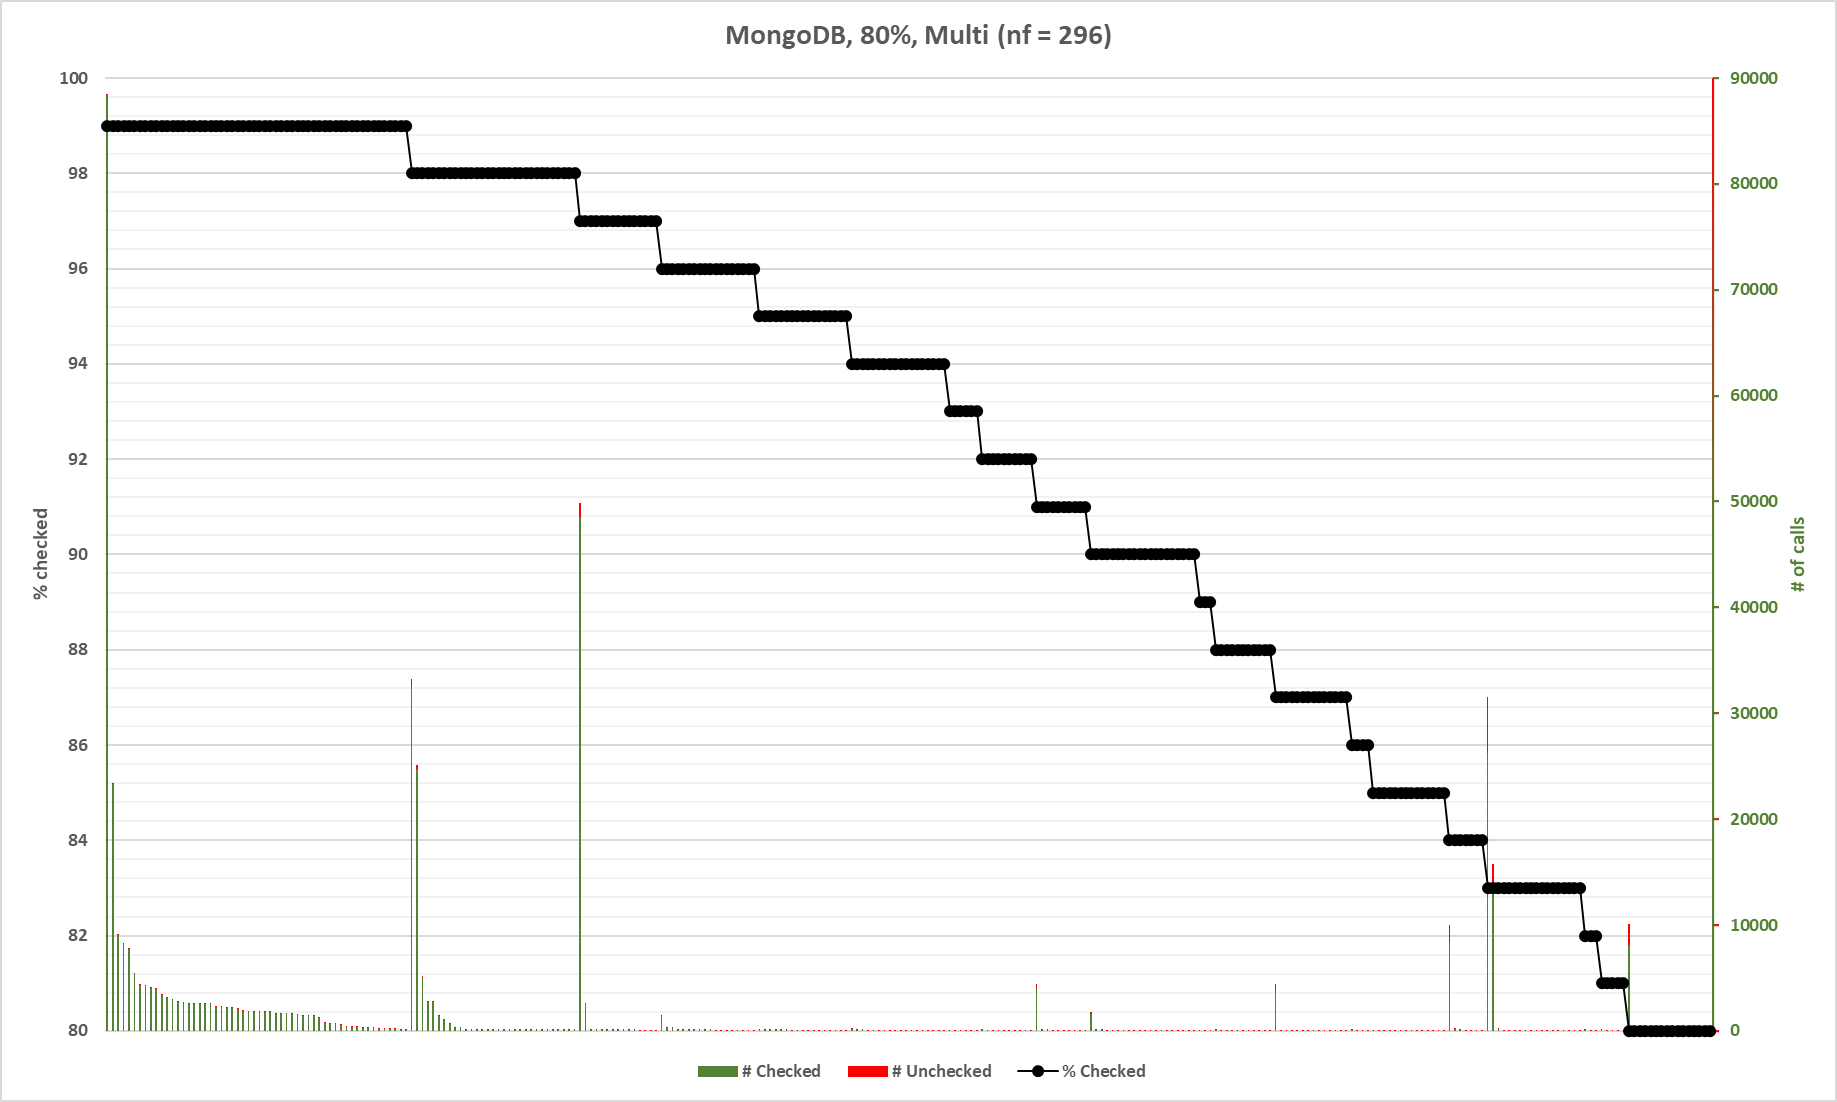
\includegraphics[width=1.2\linewidth]{images/appendix/MongoDB_80_2_Multi.png}}
\end{figure}

\begin{figure}[H]
	\makebox[\textwidth]{\includegraphics[width=1.2\linewidth]{images/appendix/OpenSSL_50_1_Single.png}}
\end{figure}

\begin{figure}[H]
	\makebox[\textwidth]{\includegraphics[width=1.2\linewidth]{images/appendix/OpenSSL_50_2_Multi.png}}
\end{figure}

\begin{figure}[H]
	\makebox[\textwidth]{\includegraphics[width=1.2\linewidth]{images/appendix/OpenSSL_80_1_Single.png}}
\end{figure}

\begin{figure}[H]
	\makebox[\textwidth]{\includegraphics[width=1.2\linewidth]{images/appendix/OpenSSL_80_2_Multi.png}}
\end{figure}

\begin{figure}[H]
	\makebox[\textwidth]{\includegraphics[width=1.2\linewidth]{images/appendix/PostgreSQL_50_1_Single.png}}
\end{figure}

\begin{figure}[H]
	\makebox[\textwidth]{\includegraphics[width=1.2\linewidth]{images/appendix/PostgreSQL_50_2_Multi.png}}
\end{figure}

\begin{figure}[H]
	\makebox[\textwidth]{\includegraphics[width=1.2\linewidth]{images/appendix/PostgreSQL_80_1_Single.png}}
\end{figure}

\begin{figure}[H]
	\makebox[\textwidth]{\includegraphics[width=1.2\linewidth]{images/appendix/PostgreSQL_80_2_Multi.png}}
\end{figure}

\begin{figure}[H]
	\makebox[\textwidth]{\includegraphics[width=1.2\linewidth]{images/appendix/ProtoBuf_50_1_Single.png}}
\end{figure}

\begin{figure}[H]
	\makebox[\textwidth]{\includegraphics[width=1.2\linewidth]{images/appendix/ProtoBuf_50_2_Multi.png}}
\end{figure}

\begin{figure}[H]
	\makebox[\textwidth]{\includegraphics[width=1.2\linewidth]{images/appendix/ProtoBuf_80_1_Single.png}}
\end{figure}

\begin{figure}[H]
	\makebox[\textwidth]{\includegraphics[width=1.2\linewidth]{images/appendix/ProtoBuf_80_2_Multi.png}}
\end{figure}

\begin{figure}[H]
	\makebox[\textwidth]{\includegraphics[width=1.2\linewidth]{images/appendix/QtBase_50_1_Single.png}}
\end{figure}

\begin{figure}[H]
	\makebox[\textwidth]{\includegraphics[width=1.2\linewidth]{images/appendix/QtBase_50_2_Multi.png}}
\end{figure}

\begin{figure}[H]
	\makebox[\textwidth]{\includegraphics[width=1.2\linewidth]{images/appendix/QtBase_80_1_Single.png}}
\end{figure}

\begin{figure}[H]
	\makebox[\textwidth]{\includegraphics[width=1.2\linewidth]{images/appendix/QtBase_80_2_Multi.png}}
\end{figure}

\begin{figure}[H]
	\makebox[\textwidth]{\includegraphics[width=1.2\linewidth]{images/appendix/SQLite_50_1_Single.png}}
\end{figure}

\begin{figure}[H]
	\makebox[\textwidth]{\includegraphics[width=1.2\linewidth]{images/appendix/SQLite_50_2_Multi.png}}
\end{figure}

\begin{figure}[H]
	\makebox[\textwidth]{\includegraphics[width=1.2\linewidth]{images/appendix/SQLite_80_1_Single.png}}
\end{figure}

\begin{figure}[H]
	\makebox[\textwidth]{\includegraphics[width=1.2\linewidth]{images/appendix/SQLite_80_2_Multi.png}}
\end{figure}

\begin{figure}[H]
	\makebox[\textwidth]{\includegraphics[width=1.2\linewidth]{images/appendix/TMux_50_1_Single.png}}
\end{figure}

\begin{figure}[H]
	\makebox[\textwidth]{\includegraphics[width=1.2\linewidth]{images/appendix/TMux_50_2_Multi.png}}
\end{figure}

\begin{figure}[H]
	\makebox[\textwidth]{\includegraphics[width=1.2\linewidth]{images/appendix/TMux_80_1_Single.png}}
\end{figure}

\begin{figure}[H]
	\makebox[\textwidth]{\includegraphics[width=1.2\linewidth]{images/appendix/TMux_80_2_Multi.png}}
\end{figure}

\begin{figure}[H]
	\makebox[\textwidth]{\includegraphics[width=1.2\linewidth]{images/appendix/tWin_50_1_Single.png}}
\end{figure}

\begin{figure}[H]
	\makebox[\textwidth]{\includegraphics[width=1.2\linewidth]{images/appendix/tWin_50_2_Multi.png}}
\end{figure}

\begin{figure}[H]
	\makebox[\textwidth]{\includegraphics[width=1.2\linewidth]{images/appendix/tWin_80_1_Single.png}}
\end{figure}

\begin{figure}[H]
	\makebox[\textwidth]{\includegraphics[width=1.2\linewidth]{images/appendix/tWin_80_2_Multi.png}}
\end{figure}

\begin{figure}[H]
	\makebox[\textwidth]{\includegraphics[width=1.2\linewidth]{images/appendix/Vim_50_1_Single.png}}
\end{figure}

\begin{figure}[H]
	\makebox[\textwidth]{\includegraphics[width=1.2\linewidth]{images/appendix/Vim_50_2_Multi.png}}
\end{figure}

\begin{figure}[H]
	\makebox[\textwidth]{\includegraphics[width=1.2\linewidth]{images/appendix/Vim_80_1_Single.png}}
\end{figure}

\begin{figure}[H]
	\makebox[\textwidth]{\includegraphics[width=1.2\linewidth]{images/appendix/Vim_80_2_Multi.png}}
\end{figure}

\begin{figure}[H]
	\makebox[\textwidth]{\includegraphics[width=1.2\linewidth]{images/appendix/Xerces-C_50_1_Single.png}}
\end{figure}

\begin{figure}[H]
	\makebox[\textwidth]{\includegraphics[width=1.2\linewidth]{images/appendix/Xerces-C_50_2_Multi.png}}
\end{figure}

\begin{figure}[H]
	\makebox[\textwidth]{\includegraphics[width=1.2\linewidth]{images/appendix/Xerces-C_80_1_Single.png}}
\end{figure}

\begin{figure}[H]
	\makebox[\textwidth]{\includegraphics[width=1.2\linewidth]{images/appendix/Xerces-C_80_2_Multi.png}}
\end{figure}
\cleardoublepage

% Bibliography (mandatory)
\phantomsection
\addcontentsline{toc}{chapter}{\biblabel}
\printbibliography[title=\biblabel]
\cleardoublepage

% List of figures (optional) - useful over 3-5 figures
\phantomsection
\addcontentsline{toc}{chapter}{\lstfigurelabel}
\listoffigures
\cleardoublepage

% List of tables (optional) - useful over 3-5 tables
\phantomsection
\addcontentsline{toc}{chapter}{\lsttablelabel}
\listoftables
\cleardoublepage

% List of algorithms (optional) - useful over 3-5 algorithms
\phantomsection
\addcontentsline{toc}{chapter}{\lstalgorithmlabel}
\listofalgorithms
\cleardoublepage

% List of codes (optional) - useful over 3-5 code samples
\phantomsection
\addcontentsline{toc}{chapter}{\lstcodelabel}
\lstlistoflistings
\cleardoublepage

% List of symbols (optional)
%\printnomenclature

\end{document}
